\chapter{Modelación física y matemática}\label{CAP4}
    
\section{Desarrollo de la modelación y métodos}
    En primero lugar, con el objetivo de modelar la cinemática y la dinámica de un robot delta de manera correcta, se presentan 2 métodos que son programados y comparados en este texto. Estos dos métodos deben dar los mismos resultados si es que son programados correctamente. Se les llama método A y método B. Cada etapas de los dos métodos tienen el mismo objetivo, sin embargo, el planteamiento del problema cinemático y dinámico es tratado de forma diferente. Para comparar los dos métodos se crea un marco de referencia global en el robot delta. Por ende, en los códigos de los algoritmos es necesario que las salidas o resultados estén en correlación a este sistema de referencia global. La figura \eqref{f:Cap4_metodologia} muestra el diagrama de flujo de los dos métodos con el objetivo de cada etapa.
    
    
\begin{figure}[htb]
    \centering
    \smartdiagramset{back arrow disabled=true,text width=2.0cm, font=\fontsize{9pt}{10pt}\selectfont}
    \smartdiagram[flow diagram:horizontal]{% 
    Nomenclatura\\ y \\sistema de referencia \\local,
    Cinematica inversa \\ Cinematica directa,
    Jacobiano,
    Cinematica \\de\\ aceleracion,
    Dinamica \\inversa
    }  
    \caption{Flujo de trabajo para el Metodo A y B}
    \label{f:Cap4_metodologia}
\end{figure}

    En segundo lugar, se explica que es el espacio de trabajo de un robot delta y los parámetros que influyen en su volumen, forma, densidad espacial, etc. Para ello, se utiliza la modelación cinemática y se privilegia el método A sobre la B por razones en relación a el cálculo del jacobiano que se explican en dicha sección.
    
    Por último, se presentan las trayectorias más comunes implementadas en el desarrollo de los robots. De todas las trayectorias presentadas se profundizan 2, las cuales se utilizan para simular el mecanismo del robot delta y comparar los resultados tanto de la modelación cinemática como de la modelación dinámica.
    
         \newpage


\section{Nomenclatura y sistema de referencia global}
    En la figura \eqref{f:ref1} se muestra el sistema de referencia global $XYZ$ y el orden de numeración de los ángulos $\theta_{i\in\{1,2,3\}}$, los cuales son utilizados para representar todos los resultados obtenidos en esta tesis. 
    
        \begin{figure}[htb]
             \centering
             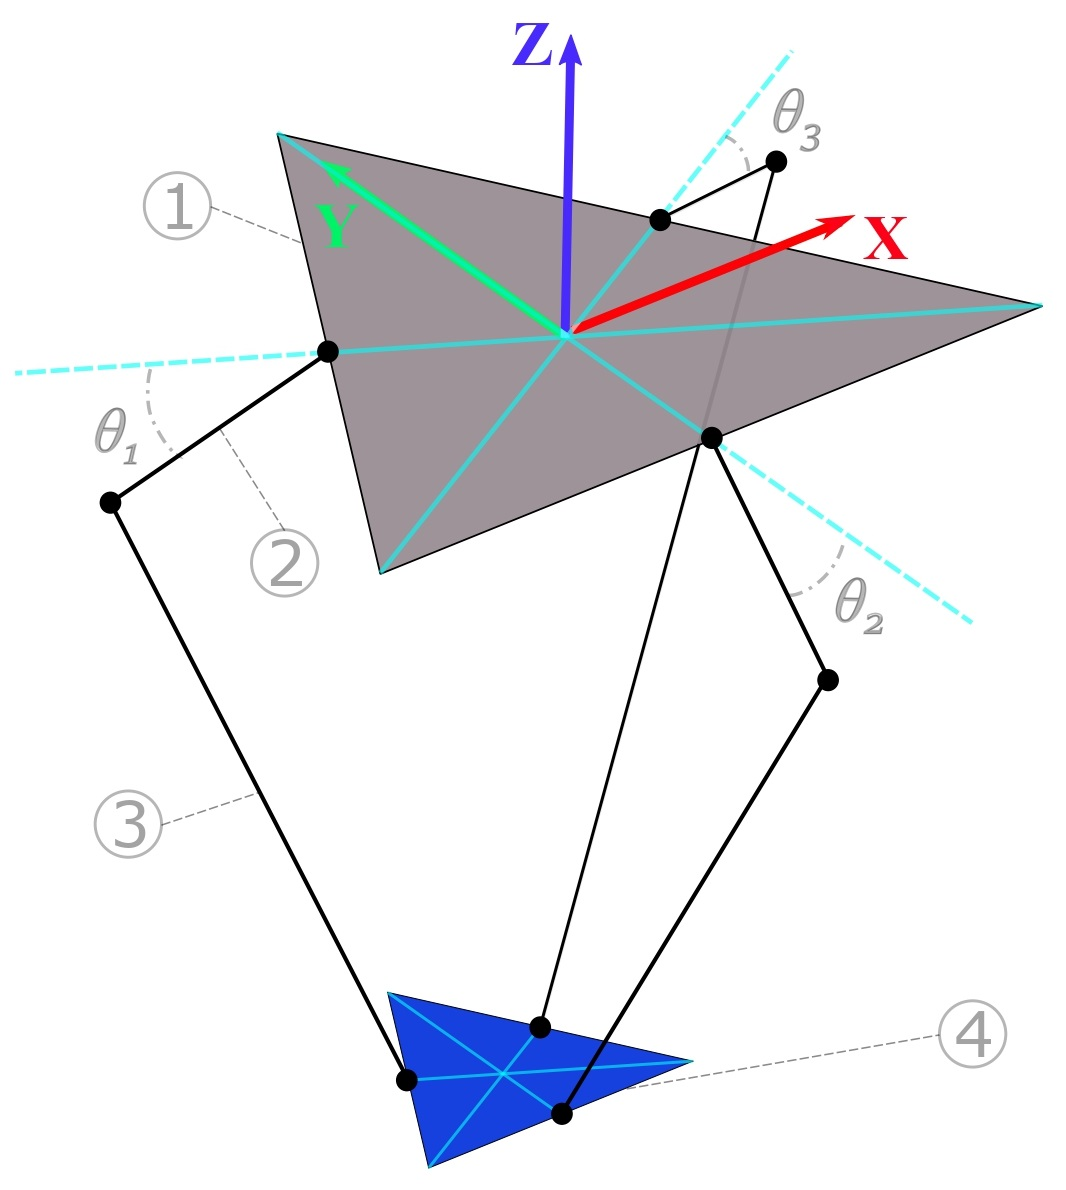
\includegraphics[width=0.73\linewidth]{Main/Chapter4/Images4/DIBUJO1.jpg}
              \caption{Sistema de referencia global $XYZ$ y angulos de los brazos $\theta_{i\in\{1,2,3\}}$ .}
              \label{f:ref1}
        \end{figure}

La tabla \eqref{tab:cap4_tabla_00} relaciona el nombre de las piezas mecánicas básicas del robot delta con su numeración en la figura \eqref{f:ref1}.
        \begin{table}[h]
            \centering
            \begin{tabular}{c c}
            \hline
                \textbf{Numero}& \textbf{Pieza Mecánica} \\ 
            \hline             \hline
             1 & Base fija \\
            \hline
             2 & Brazo \\
            \hline
             3 & Antebrazo \\
            \hline
             4 & Base Móvil\\
            \hline
            \end{tabular}
           \caption{Relación entre la numeración y piezas mecánicas de la figura  \eqref{f:ref1}.}
           \label{tab:cap4_tabla_00}
        \end{table}
        
     \newpage
     

\section{Método A}

    \subsection{Modelación cinemática de posición}
    
        En esta sección, se da a conocer una solución para calcular la cinemática inversa y cinemática directa de un robot paralelo tipo delta. Con el fin de solucionar el problema cinemático, se emplean las ideas y modelación del robot delta propuestas por Lois Rilo Antelo \cite{Diseno_e_implementacion_de_un_sistema_de_control_para_la_representacion_grafica_a_partir_de_imagenes}.
        
        \subsubsection{Nomenclatura de parámetros geométricos y sistema de referencia local}
        La figura  \eqref{f:Cap4_Metodo_A_Modelacion_Cinematica_Posicion_1}  presenta el robot delta simplificado con el respectivo sistema de referencia local $XYZ$ y el orden de numeración de los ángulos $\theta_{i\in\{1,2,3\}}$ para la solución de la cinemática de posición del método A.
        
        \begin{figure}[htb]
             \centering
             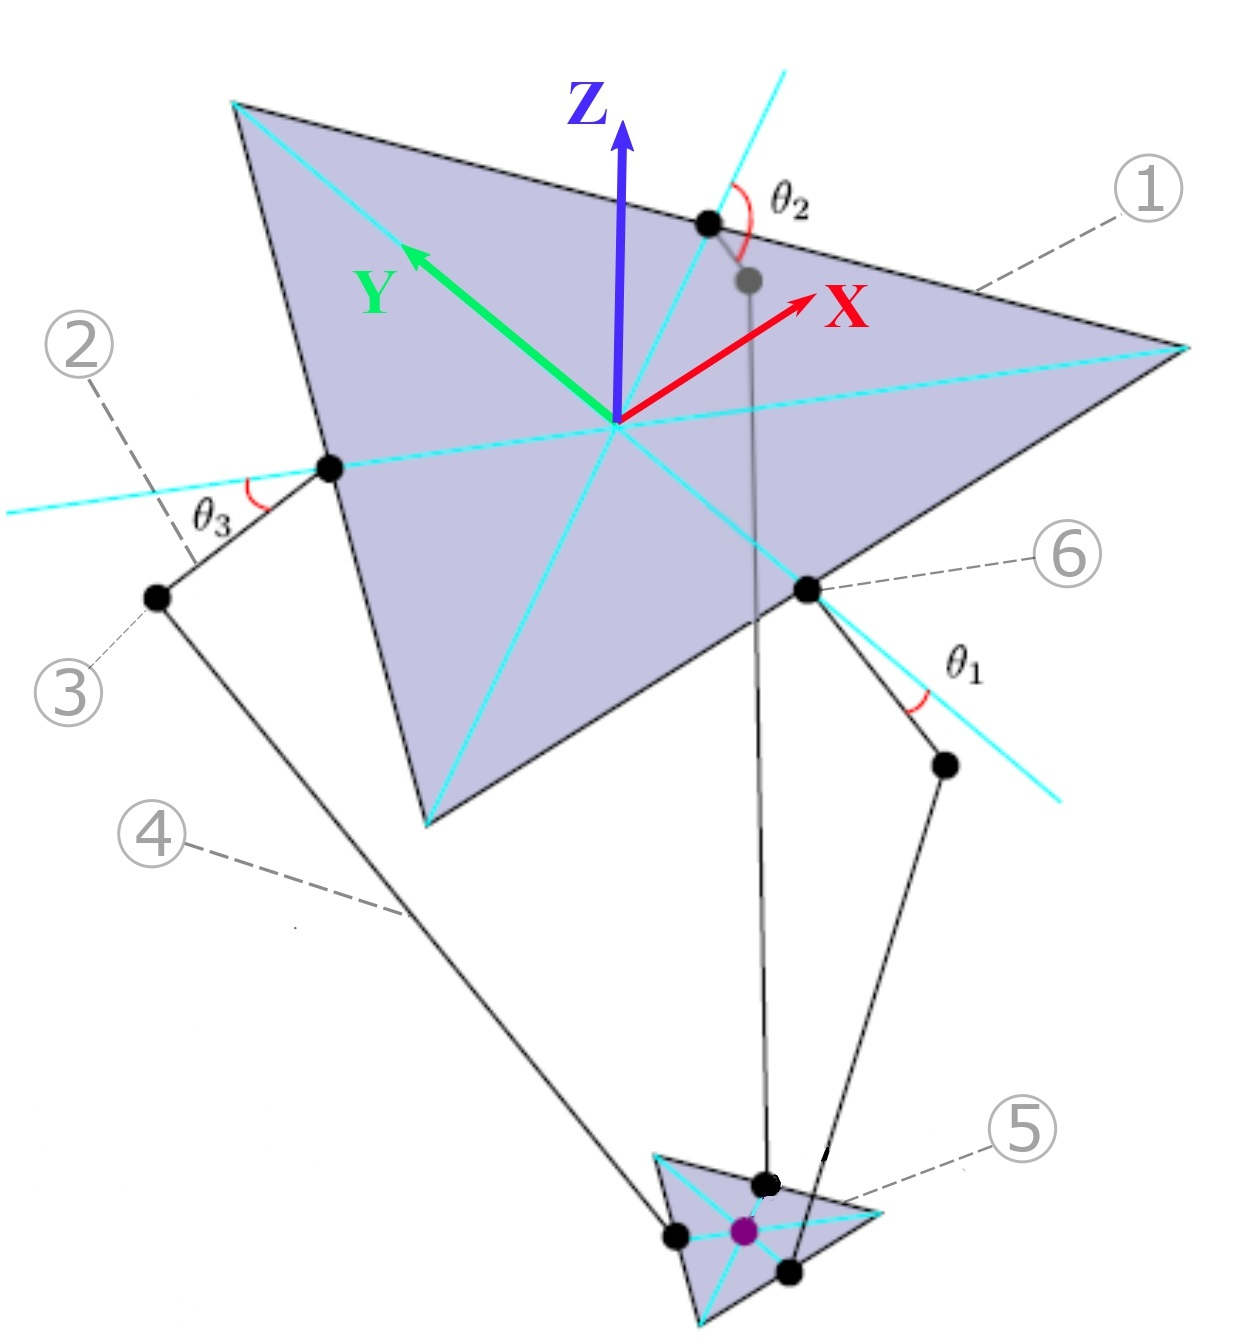
\includegraphics[width=0.5\linewidth]{Main/Chapter4/Images4/DIBUJO2.jpg}
              \caption{Sistema de referencia local para la cinemática de posición del método A \cite{Diseno_e_implementacion_de_un_sistema_de_control_para_la_representacion_grafica_a_partir_de_imagenes}. }
              \label{f:Cap4_Metodo_A_Modelacion_Cinematica_Posicion_1}
        \end{figure}

         La tabla \eqref{tab:cap4_tabla_1} muestra la relación entre la numeración en la figura \eqref{f:Cap4_Metodo_A_Modelacion_Cinematica_Posicion_1} y su nombre:
        
        \begin{table}[h]
            \centering
            \begin{tabular}{c c}
            \hline
                \textbf{Numero}& \textbf{Nombre} \\ 
            \hline             \hline
             1 & Base fija \\
            \hline
             2 & Brazo \\
            \hline
             3 & Junta esférica \\
            \hline
             4 & Antebrazo\\
            \hline
             5 & Efector final \\
             \hline
             6 & Actuador  \\
             \hline
            \end{tabular}
           \caption{Relación entre la numeración y piezas mecánicas de la figura  \eqref{f:Cap4_Metodo_A_Modelacion_Cinematica_Posicion_1}.}
           \label{tab:cap4_tabla_1}
        \end{table}

        \newpage
 
         En la figura \eqref{f:Cap4_Metodo_A_Modelacion_Cinematica_Posicion_1}  se aprecia las piezas mecánicas básicas de un robot delta, tales como la  base fija, el efector móvil y las 3 cadenas cinemáticas similares a un brazo robótico. Cada cadena esta compuestas por un actuador, que funciona como una junta revoluta, un brazo, una junta esférica que une el brazo con el antebrazo, un antebrazo y otra junta esférica que une al antebrazo con el efector final. Los 3 actuadores están situados en los puntos medios de los lados del triangulo de la base fija.
         
        La figura \eqref{f:Cap4_Metodo_A_Modelacion_Cinematica_Posicion_2} y la tabla \eqref{tab:cap4_tabla_2} presentan la nomenclatura de los principales parámetros geométricos y puntos utilizados para el desarrollo de la solución cinemática de posición:
        
        \begin{figure}[htb]
             \centering
             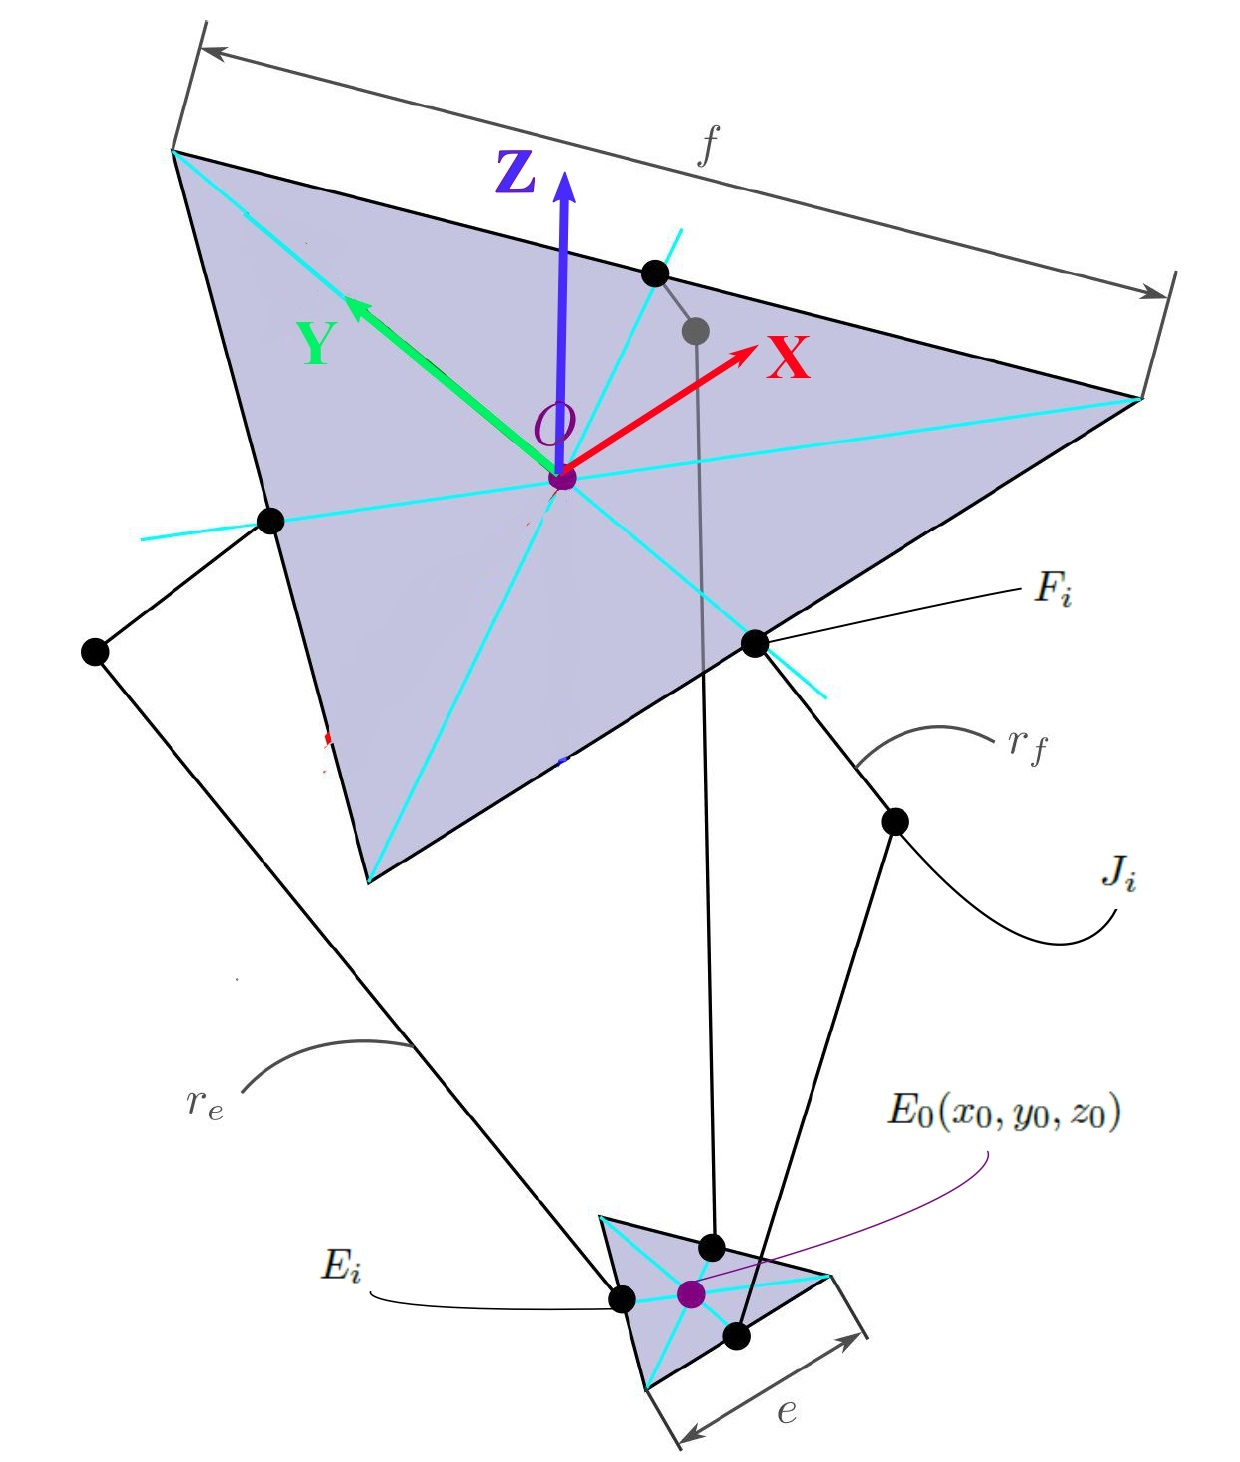
\includegraphics[width=0.43\linewidth]{Main/Chapter4/Images4/DIBUJO3.jpg}
             %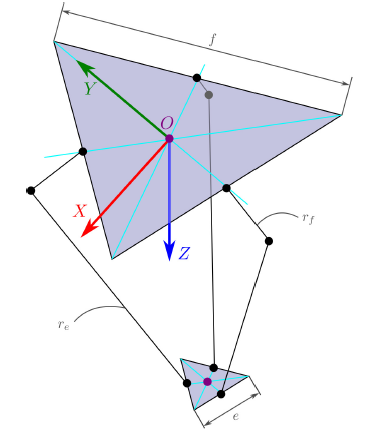
\includegraphics[width=0.6\linewidth]{Main/Chapter4/Images4/Metodo_A_Modelacion_Cinematica_Posicion_2.png}
              \caption{Principales parámetros geométricos y puntos para la cinemática de posición del método A \cite{Diseno_e_implementacion_de_un_sistema_de_control_para_la_representacion_grafica_a_partir_de_imagenes}.}
              \label{f:Cap4_Metodo_A_Modelacion_Cinematica_Posicion_2}
        \end{figure}
        

        \begingroup
            \renewcommand{\arraystretch}{1.3}
            \begin{table}[H]
            \centering
            \begin{tabular}{c m{12cm}}
               \hline
               \textbf{Simbología}  & \multicolumn{1}{c|}{\textbf{Descripción}}  \\\hline\hline
                $r_{f}$  & Longitud del brazo                                  \\\hline
               $r_{e}$  & Longitud del antebrazo                              \\\hline               
               $f$  & Lado de base fija                                \\\hline
               $e$  & Lado del efector                                   \\\hline
               $F_{i}$  & Coordenadas de la posición del actuador $i\in\{1,2,3\}$  \\\hline
               $J_{i}$  & Coordenadas de las juntas esféricas que une el brazo $i\in\{1,2,3\}$ con su antebrazo respectivo\\\hline
               $E_{i}$  & Coordenadas de las juntas esféricas que unen el antebrazo con el efector (punto medio del lado
               del triangulo que forma el efector) $i\in\{1,2,3\}$.    \\\hline
               $E_{0}(x_{0},y_{0},z_{0})$  & Coordenadas del centroide del efector   \\\hline               
            \end{tabular}
            \caption{Parámetros geométricos y puntos para cinemática de posición del método A}
            \label{tab:cap4_tabla_2}
        \end{table}
        \endgroup
        
        
        
        
        \newpage

    
        \subsubsection{Cinemática directa} \label{ma_cd}
        El fin de la cinemática directa es hallar la posición del efector final del robot delta dada una configuración articular, en este caso la posición angular de los actuadores.

        \begin{equation}
            \left({\theta }_1,{\theta }_2,{\theta }_3\right)\ \to E_0(x_0,y_0,z_0)\
        \end{equation}

        \begin{figure}[htb]
             \centering
             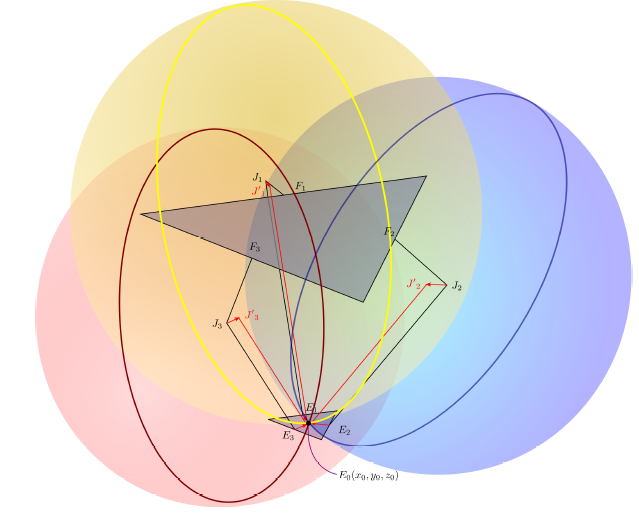
\includegraphics[width=0.8\linewidth]{Main/Chapter4/Images4/Metodo_A_Modelacion_Cinematica_Posicion_3.png}
              \caption{Sistema de ecuaciones para la cinemática directa del método A \cite{Diseno_e_implementacion_de_un_sistema_de_control_para_la_representacion_grafica_a_partir_de_imagenes}.}
              \label{f:Cap4_Metodo_A_Modelacion_Cinematica_Posicion_3}
        \end{figure}
        
        La posición en el espacio de cada brazo del robot delta ya esta definida gracias a que se conocen los ángulos de los actuadores $({\theta }_1,{\theta }_2,{\theta }_3)$ y la longitud de los brazos $r_f$. 
        
        Por otro lado, sobre los antebrazos solo se conoce la posición de las juntas esféricas $J_i$ que los une con los brazos. Como resultado del incompleto conocimiento espacial de estas piezas, la posición y orientación de cada antebrazo esta restringida por esferas con centro en la junta esférica $J_i$ y radio equivalente al largo de cada antebrazo $r_e$. 
        
        Para finalizar, se realiza una traslación de las esferas mencionadas anteriormente para obtener las coordenadas del centroide del efector final $E_0$. Esta translación produce 3 nuevas esferas, con nuevos centros y de radio equivalente al largo del antebrazo $r_e$. Las nuevas esferas se intersecan en el centroide del efector $E_0$ .Como último paso, para calcular las coordenadas del punto $E_0(x_0,y_0,z_0)$ se realiza un sistema de ecuaciones no lineal con 3 restricciones (esferas que contienen los antebrazos) y 3 incógnitas (coordenadas $(x_0,y_0,z_0)$ del efector final) .

        \newpage
        
        Los 3 centros de las nuevas esferas de radio $r_e$ que se intersecan en el centroide del efector $E_0(x_0,y_0,z_0)$ son:
        
    \vspace{-1em}

        \begin{center}
        \renewcommand{\arraystretch}{2.5}
        
            \begin{table}[H]
            \centering
            \begin{tabular}{p{1.4cm} c c } 
                 \hline
                 \textbf{Centros}  &  \textbf{Centros  de esferas} \\ [0.1ex] 
                 \hline\hline
                         $\left(x_1,y_1,z_1\right)$ &
                         ${J^'}_1\left(0,\left[-\frac{f-e}{2\sqrt{3}}-r_f{\mathrm{cos} \left({\theta }_1\right)\ }\right],-r_f{\mathrm{sin} \left({\theta }_1\right)\ }\right)$ \\ 
                \hline
                          $\left(x_2,y_2,z_2\right)$ & ${J^'}_2\left(\left[\frac{f-e}{2\sqrt{3}}+r_f{\mathrm{cos} \left({\theta }_2\right)\ }\right]\mathrm{cos}\mathrm{}(30{}^\circ ),\left[\frac{f-e}{2\sqrt{3}}+r_f{\mathrm{cos} \left({\theta }_2\right)\ }\right]\mathrm{sin}\mathrm{}(30{}^\circ ),-r_f{\mathrm{sin} \left({\theta }_2\right)\ }\right)$\\
                \hline
                           $\left(x_3,y_3,z_3\right)$ & ${J^'}_3\left(-\left[\frac{f-e}{2\sqrt{3}}+r_f{\mathrm{cos} \left({\theta }_3\right)\ }\right]\mathrm{cos}\mathrm{}(30{}^\circ ),\left[\frac{f-e}{2\sqrt{3}}+r_f{\mathrm{cos} \left({\theta }_3\right)\ }\right]\mathrm{sin}\mathrm{}(30{}^\circ ),-r_f{\mathrm{sin} \left({\theta }_3\right)\ }\right)$\\
                 \hline
            \end{tabular}
            \caption{Posición de los centros de las esferas originadas por la traslación de las juntas $J_i$ }
            \label{tab:cap4_tabla_3}
            \end{table}
        \end{center}
        
    \vspace{-3.5em}

    Para simplificar las ecuaciones algebraicas de las esferas, se escriben los centros con la nomenclatura $\left(x_i,y_i,z_i\right)\ $ donde $i\in\{1,2,3\}$. El sistema de ecuaciones es:
    
        \vspace{-1em}

    
    \begin{equation}
    \left\lbrace
    \begin{array}{ll}
    {\left(x-x_1\right)}^2+{\left(y-y_1\right)}^2\ +{\left(z-z_1\right)}^2=\ {r_e}^2\  \\ 
    {\left(x-x_2\right)}^2+{\left(y-y_2\right)}^2\ +{\left(z-z_2\right)}^2=\ {r_e}^2 \\ 
    {\left(x-x_3\right)}^2+{\left(y-y_3\right)}^2\ +{x\left(z-z_3\right)}^2=\ {r_e}^2
    \end{array}
    \right.
    \label{eq:cap4_eq_2}
    \end{equation}


    Despu\'{e}s de un extenso desarrollo alg\'{e}brico, la soluci\'{o}n del sistema de ecuaciones \eqref{eq:cap4_eq_2} es:

    \vspace{-2.5em}

    \begin{align}
    \begin{split}
            E_0\left(x_0,y_0,z_0\right)&={} \left(a_1z+\ b_1,a_2z+\ b_2,\frac{-B-\ \sqrt{\left(B^2\right)-\left(4AC\right)}}{2*A}\right)\\
    \end{split}
    \label{eq:cap4_eq_3}
    \end{align}
    

    Donde:
    \vspace{-1.0em}
        
    \begin{align}
        z={}& \frac{-B-\ \sqrt{\left(B^2\right)-\left(4AC\right)}}{2A}
        \label{eq:cap4_eq_4} \\
        A={}& {a_1}^2+{a_2}^2+1
        \label{eq:cap4_eq_5} \\
        B={}&  2\left(a_1(b_1-x_1)+a_2(b_2-y_1)-z_1\right)
        \label{eq:cap4_eq_6} \\
        C={}& ({(b_1-x_1)}^2+{(b_2-y_1)}^2+{z_1}^2- {r_e}^2) 
        \label{eq:cap4_eq_7} \\
        a_1={}& \frac{\left(z_2-z_1\right)\left(y_3-y_1\right)-\left(z_3-z_1\right)\left(y_2-y_1\right)}{d} 
        \label{eq:cap4_eq_8} \\
        b_1={}& \left(\frac{1}{2*(-d)}\right)*\left(\left(w_2 - w_1\right)\left(y_3-y_1\right)-\left(w_3 - w_1\right)\left(y_2-y_1\right)\right)
        \label{eq:cap4_eq_9} \\
        a_2={}& \frac{-1}{d}*\left[\left(z_2-z_1\right)x_3-(z_3-z_1)x_2+(z_3-z_2)x_1\right]
        \label{eq:cap4_eq_10} \\
        b_2={}& \frac{1}{2d}*[\left(w_2-w_1\right)x_3-\left(w_3-w_1\right)x_2+\left(w_3-w_2)x_1\right]
        \label{eq:cap4_eq_11} \\
        d={}& \left(y_2- y_1\right)x_3-\left(y_3-y_1\right)x_2- \left(y_2-y_3\right)x_1
        \label{eq:cap4_eq_12} \\
        w_i={}& {x_i}^2+{y_i}^2 +{z_i}^2
        \label{eq:cap4_eq_13} 
    \end{align}

         \newpage


        \subsubsection{Cinemática inversa} \label{ma_ci}
        El objetivo de la cinemática inversa es hallar la posición de los actuadores en el espacio articular dada la posición cartesiana del centroide del efector final.
        
        \begin{equation}
            E_0(x_0,y_0,z_0)\ \to \left({\theta }_1,{\theta }_2,{\theta }_3\right)
        \end{equation}
        
        
        \begin{figure}[htb]
             \centering
             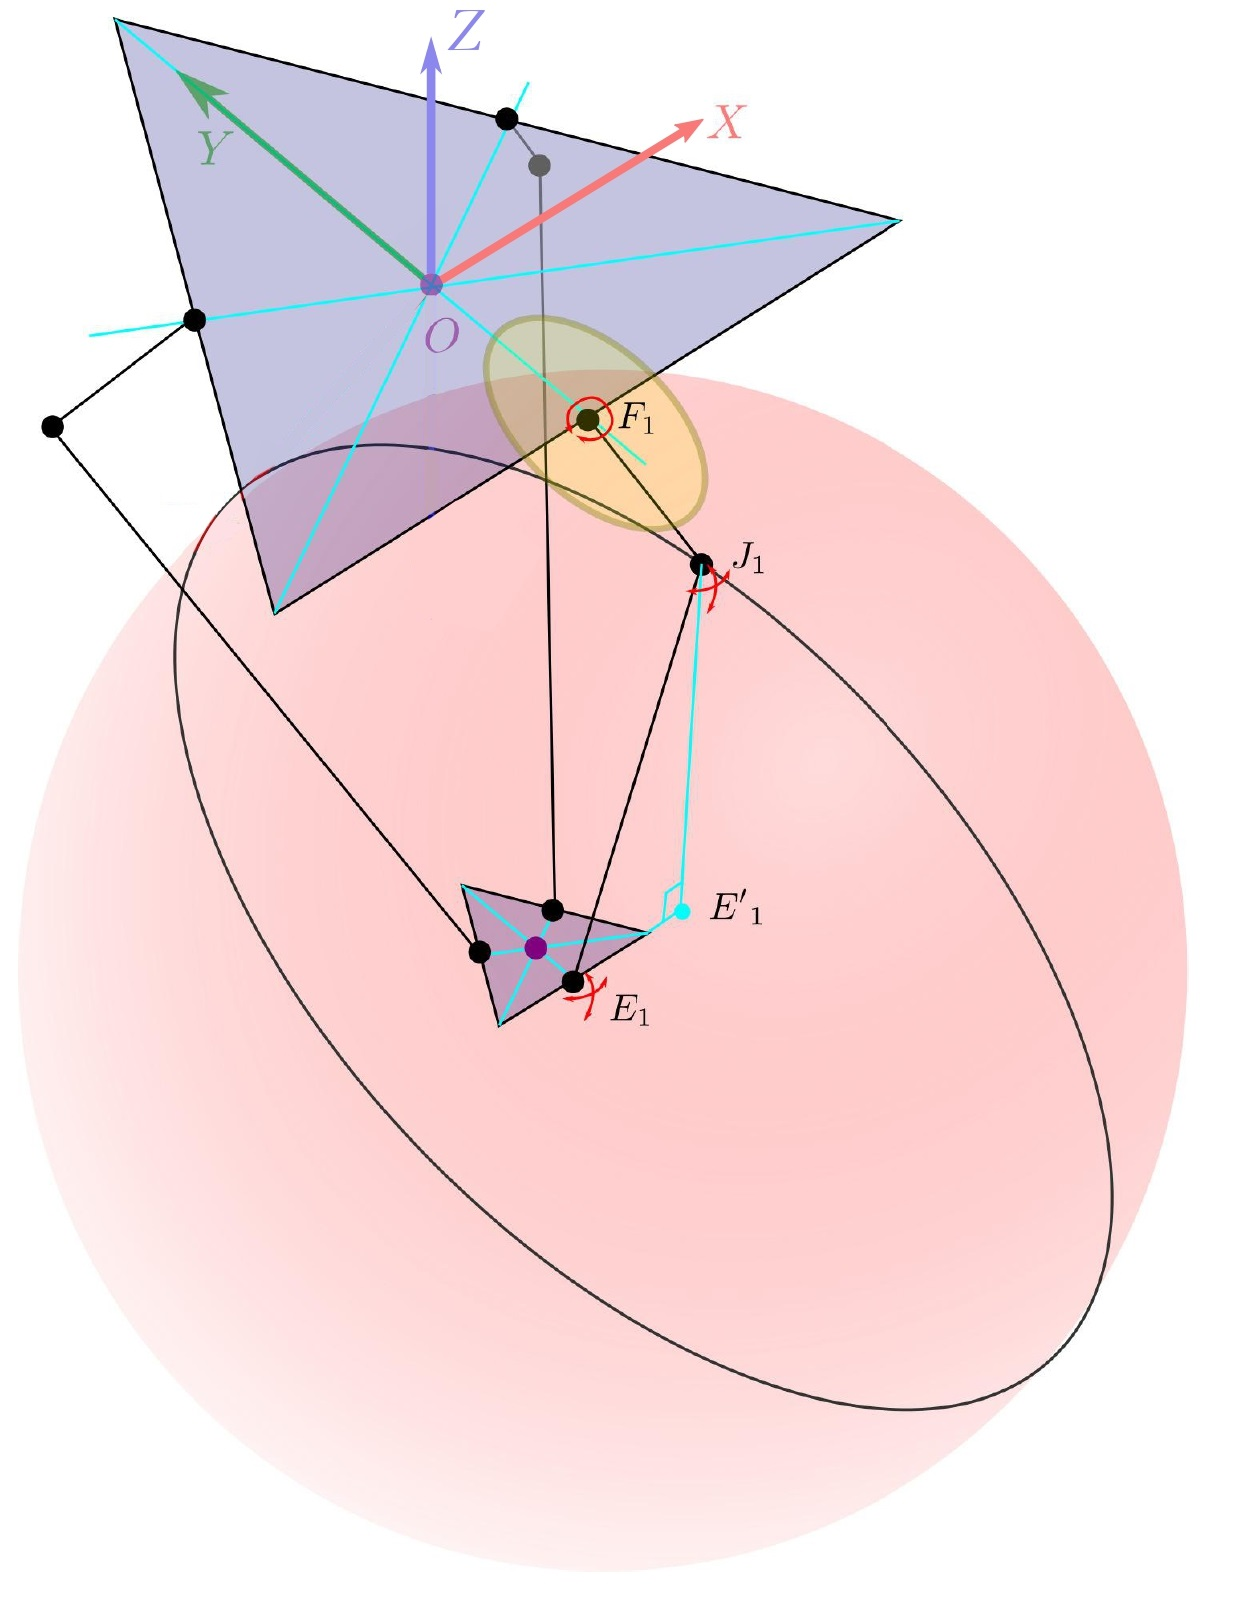
\includegraphics[width=0.43\linewidth]{Main/Chapter4/Images4/DIBUJO6.jpg}
              \caption{Sistema de ecuaciones para la cinemática inversa del método A \cite{Diseno_e_implementacion_de_un_sistema_de_control_para_la_representacion_grafica_a_partir_de_imagenes}.}
              \label{f:Cap4_Metodo_A_Modelacion_Cinematica_Posicion_4}
        \end{figure}
        
         Se tiene la informaci\'{o}n de las coordenadas de las juntas esf\'{e}ricas $E_i$ a causa de que se sabe la posici\'{o}n centroide del efector final $E_0(x_0,y_0,z_0)$ y que cada lado del tri\'{a}ngulo formado por la base fija son paralelos a los lados del triangulo formado por el efector, es decir, tanto la orientaci\'{o}n como la inclinaci\'{o}n entre la base fija y el efector son iguales.  

        En relaci\'{o}n con los antebrazos, solo se conoce el punto $E_i$ , que coincide con las posiciones de cada junta esf\'{e}rica unida al efector. Esto trae como consecuencia que cada antebrazo esta restringido por esferas con centros en las juntas esf\'{e}ricas $E_i$ con radio equivalente al largo del antebrazo $r_e$.
    
        Acerca de los brazos solo se tiene conocimiento de los puntos $F_i$, que son la posici\'{o}n de cada actuador. Los actuadores son juntas revolutas y restringen le movimiento de cada brazo en un plano. La configuraci\'{o}n espacial de estos planos para cada cadena cinem\'{a}tica es determinada por los puntos $F_i$ ,$O$ (origen) y el plano de la que contiene la base fija. El plano que contiene la base fija es perpendicular a los planos que restringen el movimiento de los brazos. En consecuencia, la posici\'{o}n de los puntos extremos de cada brazo, es decir, los puntos $J_i$ (junta esf\'{e}rica), est\'{a}n restringidos por circunferencia como se muestra en la figura \eqref{f:Cap4_Metodo_A_Modelacion_Cinematica_Posicion_4} .

                \newpage

        Para finalizar, se calcula la intersecci\'{o}n entre las circunferencias para cada cadena cinem\'{a}tica, en otras palabras, los puntos  $J_i$ . Una vez obtenida la posici\'{o}n de las 3 juntas $J_i$, con algebra simple se calculan los angulos ${\theta }_1,{\theta }_2$ y ${\theta }_3$.
        
        En el caso del actuador  $i=1$ , los centros de las circunferencias que se intersecan en la junta esf\'{e}rica $J_1$ son:
        
        \begin{center}
        \renewcommand{\arraystretch}{2.5}
        
            \begin{table}[H]
            \centering
            \begin{tabular}{p{1.4cm} c c } 
                 \hline
                 \textbf{Centros}  &  \textbf{Centros esferas}  & \textbf{Radio} \\ [0.1ex] 
                 \hline\hline
                         $\left(y_1,z_1\right)$ &
                        $F_1\left(y_{F_1}\,z_{F_1}\right)=\left(-\frac{f}{2\sqrt{3}},0\right)$\textit{} & 
                                                 $r_f$  \\ 
                \hline
                          $(y_2,z_2)$&
                          ${E^'}_{1}$ $(y_{{E^'}_1}$ $z_{{E^'}_1}$ $)=(y_0-\frac{e}{2\sqrt{3}},z_0)$ &
                          $r_2=\sqrt{{r_e}^2-{x_o}^2}$ \\
                \hline
            \end{tabular}
            \caption{Coordenadas del centro de las esferas y sus radios utilizados para la solución de la cinemática inversa del método A.}
            \label{tab:cap4_tabla_4}
            \end{table}
        \end{center}
    \vspace{-2.5em}
        
Las ecuaciones cartesianas de las dos circunferencias quedan representadas en términos de  $y_{1},z_{1},r_{f},r_{f},~y_{2},z_{2},\sqrt[]{r_{e}^{2}-x_{o}^{2}}$  para simplificar la escritura de los cálculos:

    \begin{equation}
    \left\lbrace
    \begin{array}{ll}
    \left( y-y_{1} \right) ^{2} + \left( z-z_{1} \right) ^{2}= r_{f}^{2}~\\
    \left( y-y_{2} \right) ^{2} + \left( z-z_{2} \right) ^{2}= r_{e}^{2}-x_{o}^{2}\\ 
    \end{array}
    \right.
    \label{eq:cap4_eq_15}
    \end{equation}

La solución del sistema de ecuaciones \eqref{eq:cap4_eq_15} es:

    \begin{equation}
    J_{1}= \left( x_{J_{1}},y_{J_{1}},z_{J_{1}} \right) = \left( 0,y,a+by \right)
    \label{eq:cap4_eq_16}
    \end{equation}

    Donde:

    \begin{equation}
        y=\frac{\left( y_{1}-ab \right) -\sqrt[]{ \left[  -\left( a+by_{1} \right) ^{2}+ \left( b^{2}+1 \right) r_{f}^{2} \right] }}{ \left( b^{2}+1 \right) }
    \label{eq:cap4_eq_17}
    \end{equation}

    \begin{equation}
        b=\frac{ \left( y_{1}-y_{2} \right) }{z_{2}}~ 
    \label{eq:cap4_eq_18}
    \end{equation}
    
    \begin{equation}
        a= \frac{x_{o}^{2}+y_{2}^{2}+z_{0}^{2}+r_{f}^{2}- r_{e}^{2}~-y_{1}^{2}}{2z_{0}} 
    \label{eq:cap4_eq_19}
    \end{equation}

                \newpage

En último lugar, se determina el ángulo \( ~ \theta _{1} \)  por medio del triángulo rectángulo formado en el brazo y la proyección del mismo en el plano $XY$:

    \begin{equation}
        \theta _{1}=\arctan  \left( ~\frac{z_{J_{1}}}{y_{F_{1}}-y_{J_{1}}} \right)  
        \label{eq:cap4_eq_20}
    \end{equation}
    
    Donde:  \( y_{F_{1}}= - \frac{f}{2~\sqrt[]{3}} \)

    
        \begin{figure}[htb]
             \centering
             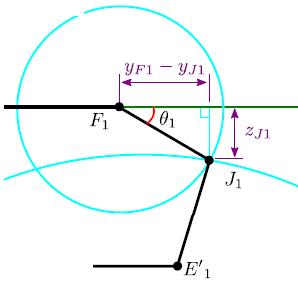
\includegraphics[width=0.37\linewidth]{Main/Chapter4/Images4/DIBUJO4.png}
              \caption{Intersección entre circulos en punto $J_1$ y proyección del punto $E_1$ sobre el plano XY  \cite{Diseno_e_implementacion_de_un_sistema_de_control_para_la_representacion_grafica_a_partir_de_imagenes}.}
              \label{f:Cap4_Metodo_A_Modelacion_Cinematica_Posicion_5}
        \end{figure}


Se emplea el mismo procedimiento anterior para encontrar los ángulos  \(  \theta _{2} \)  y  \(  \theta _{3} \)  por medio de matrices de rotación, con un ángulo de rotación de $120 ^{\circ} $  para la cadena cinemática con el actuador 2 y de $240 ^{\circ} $  para la cadena cinemática con el actuador 3. Estas matrices giran el sistema de referencia local en $120 ^{\circ} $  y $240 ^{\circ} $ . 

        \begin{figure}[htb]
             \centering
             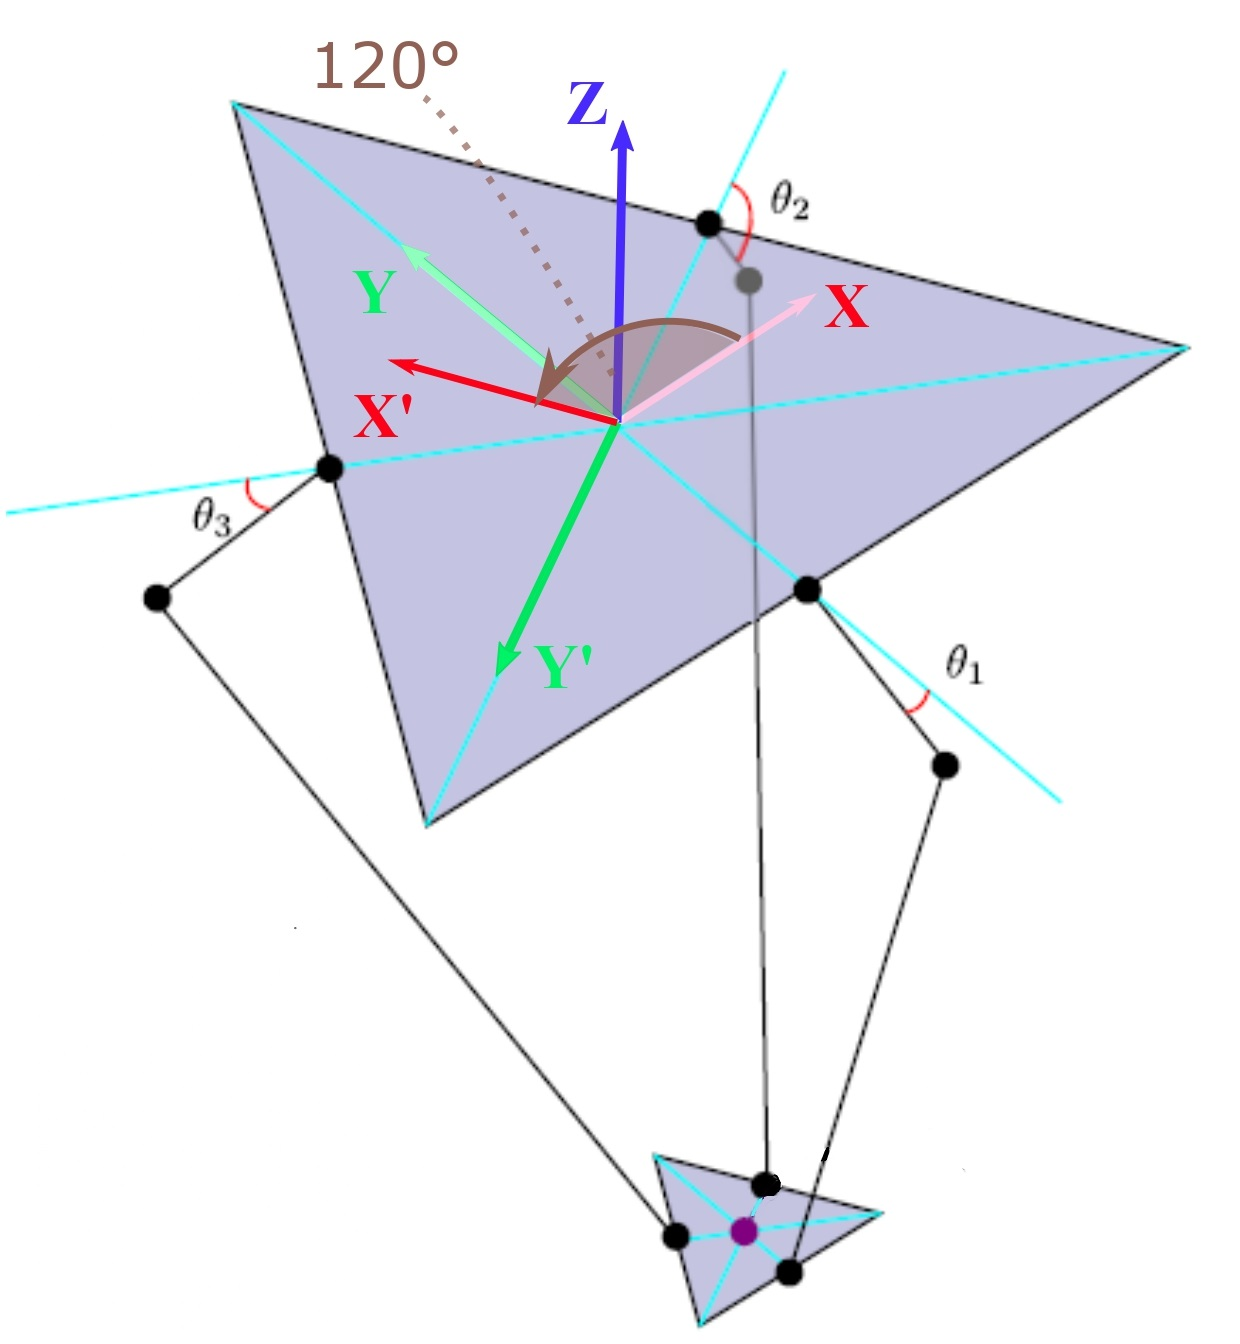
\includegraphics[width=0.49\linewidth]{Main/Chapter4/Images4/DIBUJO5.jpg}
              \caption{Rotación del sistema de referencia local en $120 ^{\circ} $  para la solución de la cinemática inversa del método A \cite{Diseno_e_implementacion_de_un_sistema_de_control_para_la_representacion_grafica_a_partir_de_imagenes}.}
              \label{f:Cap4_Metodo_A_Modelacion_Cinematica_Posicion_6}
        \end{figure}

        \newpage

    \subsection{Modelación cinemática de la velocidad}\label{ma_cvel}
        En esta sección, se da a conocer un método para calcular la matriz jacobiana y su estrecha relación con las singularidades de un robot paralelo tipo delta. Se implementan las ideas extraídas del paper \cite{Hsu_modelling_ai}.
    
        \subsubsection{Nomenclatura de parámetros geométricos y sistema de referencia local}
        
        En la figura \eqref{f:Cap4_Metodo_A_Modelacion_Cinematica_Posicion_7} se visualizan 3 cadenas cinemáticas las cuales se componen de 4 partes mecánicas: la base fija, los brazos accionados, las barras seguidoras y la plataforma móvil.
        
        \begin{figure}[htb]
             \centering
             %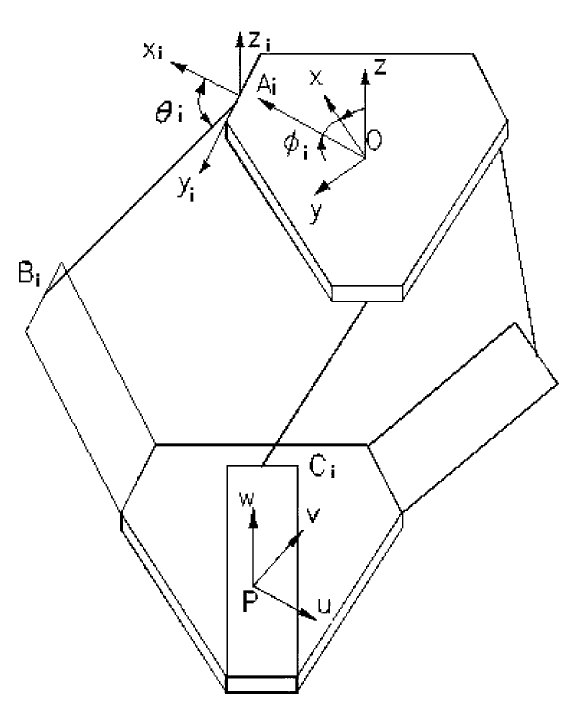
\includegraphics[width=0.45\linewidth]{Main/Chapter4/Images4/Metodo_A_Modelacion_Cinematica_Posicion_7.png}
             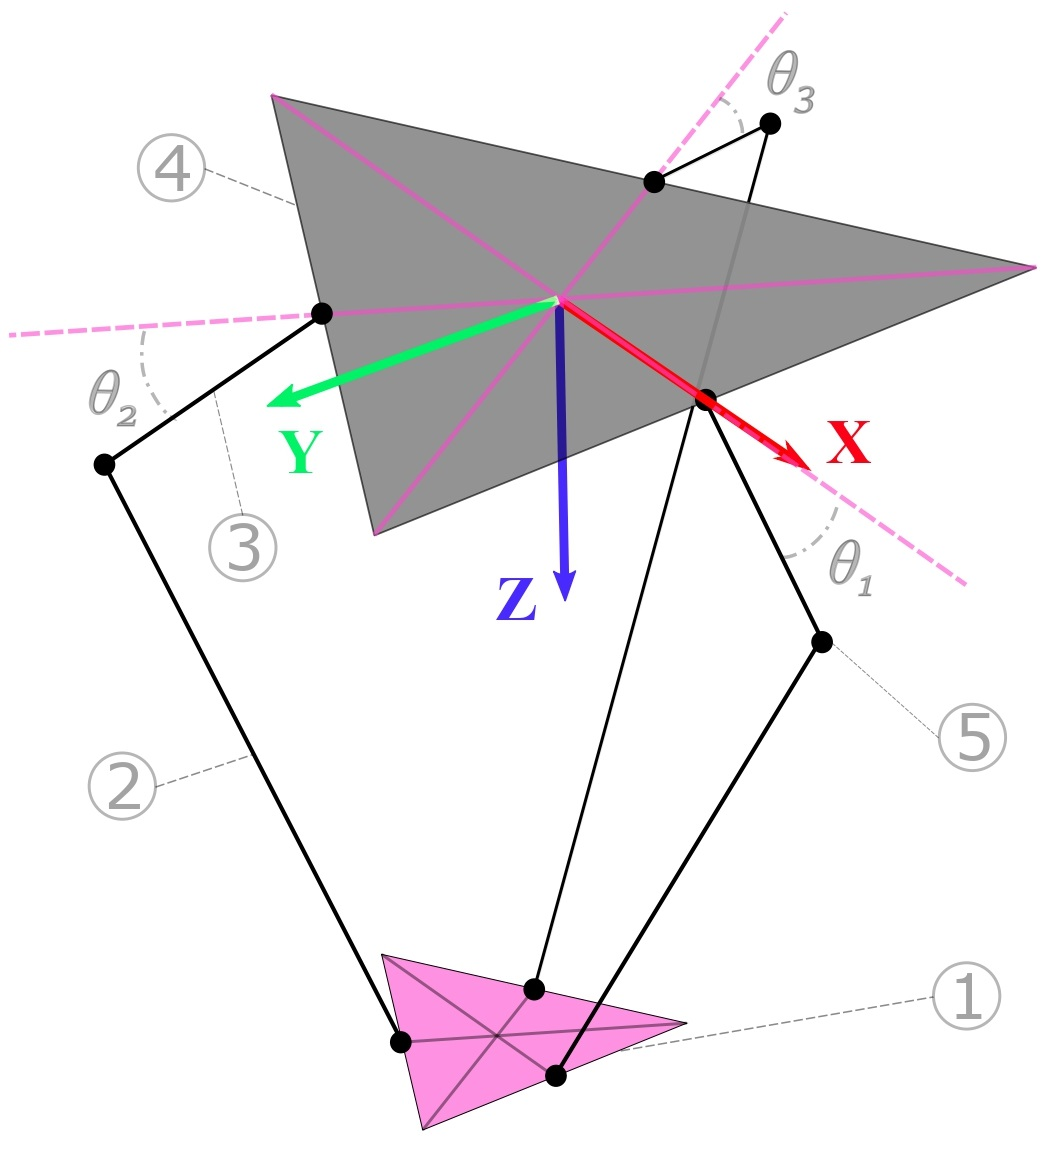
\includegraphics[width=0.62\linewidth]{Main/Chapter4/Images4/DIBUJO18.jpg}
              \caption{Sistema de referencia local para la cinemática de velocidad del método A. }
              \label{f:Cap4_Metodo_A_Modelacion_Cinematica_Posicion_7}
        \end{figure}
 
          La tabla \eqref{tab:cap4_tabla_5} muestra la relación entre la numeración en la figura \eqref{f:Cap4_Metodo_A_Modelacion_Cinematica_Posicion_7}  y su nombre.
        
        \begin{table}[h]
            \centering
            \begin{tabular}{c c}
            \hline
                \textbf{Numero}& \textbf{Nombre} \\ 
            \hline             \hline
             1 & plataforma móvil \\
            \hline
             2 & barras seguidoras \\
            \hline
             3 & brazos accionados \\
            \hline
             4 & base fija\\
            \hline
             5 & Juntas universales \\
             \hline
            \end{tabular}
           \caption{Relación entre la numeración y piezas mecánicas de la figura  \eqref{f:Cap4_Metodo_A_Modelacion_Cinematica_Posicion_7}}
           \label{tab:cap4_tabla_5}
        \end{table}
        
        \newpage
        
     Cada cadena contiene una junta giratoria activada por actuadores en la base fija en la posición donde se conectan los brazos accionados. Cada brazo accionado está conectado a 2 barras seguidoras a través de juntas de 3 grados de libertad. Las juntas son una combinación de junta universal y cojinete.  Las barras seguidoras también están conectadas a la plataforma móvil a través del mismo tipo de juntas de 3 grados de libertad, es decir, una combinación de junta universal y cojinete.

      

        Como se muestra en la figura \eqref{f:Cap4_Metodo_A_Modelacion_Cinematica_Posicion_71}, un sistema de referencia $O-xyz$ se adjunta al centro $O$ de la plataforma fija, donde los ejes $x$ e $y$ se encuentran en el plano fijo y el eje $z$ apunta hacia abajo verticalmente.
        Otro sistema de referencia $A_i$ -  $x_iy_iz_i$  se adjunta a la base fija en el punto $A_i$, de modo que el eje $x_i$ está colineal con la línea extendida $OA_i$, el eje $y_i$ se dirige a lo largo del eje de la articulación giratoria en $A_i$ y el eje $z_i$ es paralelo al eje $Z$. 
        Los angulos $\phi_{i\in\{1,2,3\}}$ se mide desde el eje $x$ al eje $x_i$, y son parámetros constantes del diseño del manipulador.  
    
    


        \begin{figure}[htb]
             \centering
             %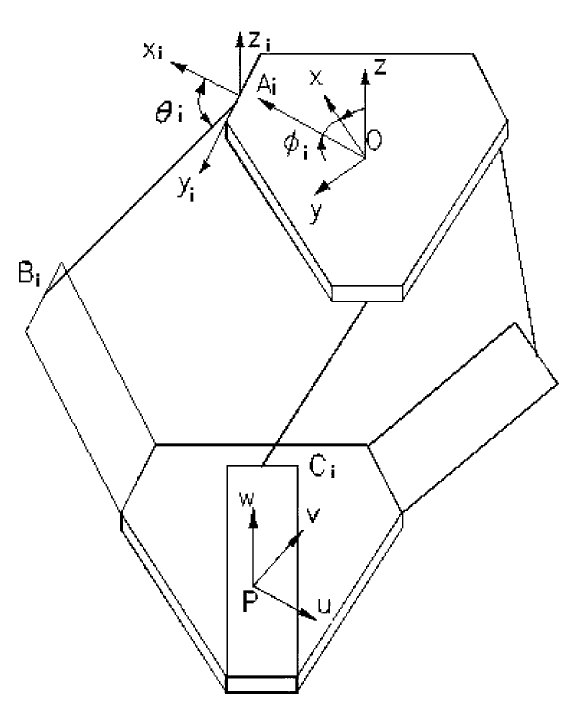
\includegraphics[width=0.45\linewidth]{Main/Chapter4/Images4/Metodo_A_Modelacion_Cinematica_Posicion_7.png}
             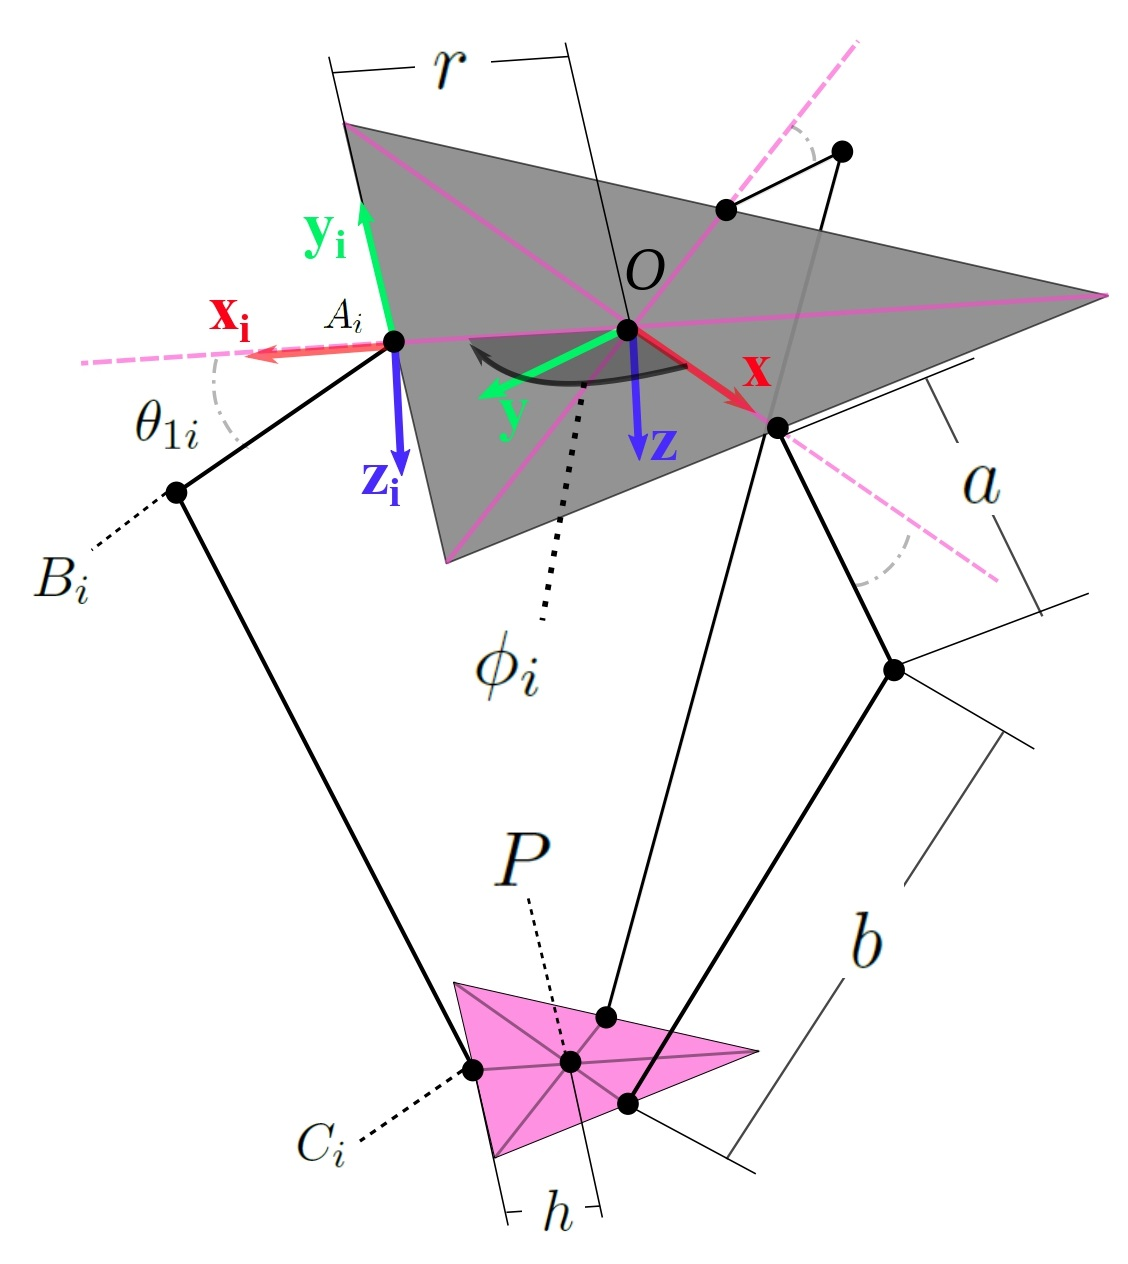
\includegraphics[width=0.8\linewidth]{Main/Chapter4/Images4/DIBUJO19.jpg}
              \caption{Traslación y rotación del sistema de referencia local $O$ - $xyz$ en $120^{\circ}$ para la solución de la cinemática de velocidad del metodo A. }
              \label{f:Cap4_Metodo_A_Modelacion_Cinematica_Posicion_71}
        \end{figure}
        
            \newpage


      La tabla \eqref{tab:cap4_tabla_6} presenta la simbología de las principales longitudes, puntos, ángulos y sistemas de referencia para el desarrollo de la solución cinemática de velocidad:
 
        \begingroup
            \renewcommand{\arraystretch}{2.0}
            \begin{table}[H]
            \centering
            \begin{tabular}{c m{12cm}}
               \hline
               \textbf{Simbología}  & \multicolumn{1}{c}{\textbf{Descripción}}  \\
               \hline           \hline            
             $a$ & Longitud de los brazos accionados \\
            \hline
             $b$ & Longitud de las barras seguidoras \\
            \hline
             $r$ & Longitud desde el centro de la base fija a un actuador $i\in\{1,2,3\}$ \\
            \hline
             $h$ & Longitud del centro de la plataforma móvil a una junta universal unida a él.\\
            \hline
             $A_{i}$ & Punto que representa la posición de actuador $i\in\{1,2,3\}$ \\
            \hline
             $ B_{i}$ & Punto que representa la posición de las juntas universales que unen los brazos accionados y las barras seguidoras \\
            \hline
             $C_{i}$ & Punto que representa la posición de las juntas universales que unen las barras seguidoras con la plataforma móvil \\
            \hline
             $P$ & Punto que representa el centro de la plataforma móvil.\\
            \hline
              & Ángulo que representa la posición angular de los 3 actuadores sobre el plano de la base fija $ \phi _{i} \in \{  0 ^{\circ}  , 120 ^{\circ}  , 240 ^{\circ} \} $ \\
            \hline
             $ \theta _{1i}$ & Ángulo que representa la posición angular de las barras accionadas respecto al eje que contiene los puntos del origen del sistema de referencia local y punto $A_{i}$  \\
            \hline
             $O$ – $xyz$ & Sistema de referencia local\\
            \hline
             $  A_{i}$ – $x_{i}y_{i}z_{i}$ & Sistema de referencia local trasladado y rotado a los puntos $A_{i}$ dependiendo del ángulo $\phi _{i}$.  \\
            \hline
            \end{tabular}
            \caption{Simbología y descripción de las longitudes, puntos, ángulos y sistemas de referencia para el desarrollo de la solución cinemática de velocidad del método A.}
           \label{tab:cap4_tabla_6}
        \end{table}
        \endgroup        
        
    \newpage

        \subsubsection{Vectorización y ángulos de las articulaciones} \label{cap4_angulosinteriores}
        
        La figura \eqref{f:Cap4_Metodo_A_Modelacion_Cinematica_Posicion_8} define los ángulos de articulación internos asociados con la extremidad  \( i \) . El ángulo \(  \theta _{2i} \)  se define desde la línea extendida de  \( \overrightarrow{A_{i}B_{i}} \)  hasta la línea definida por la intersección del plano del paralelogramo y el plano  \( A_{i} - x_{i}z_{i} \). El ángulo \(  \theta _{3i} \)  se mide desde la dirección del eje \( y_{i} \)  hasta  el vector \( \overrightarrow{B_{i}C_{i}} \) .
        
        \begin{figure}[htb]
             \centering
             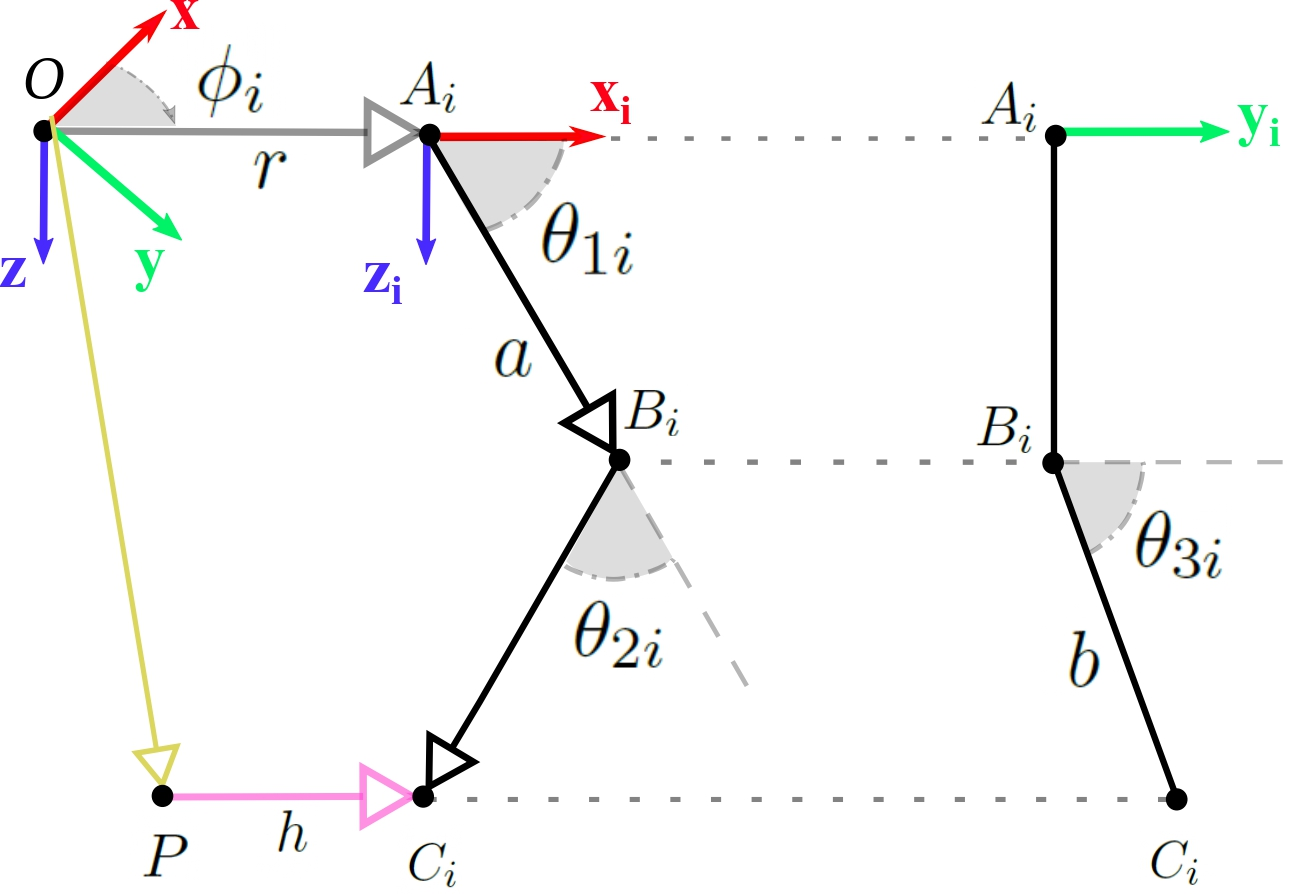
\includegraphics[width=0.96\linewidth]{Main/Chapter4/Images4/DIBUJO21.jpg}
              \caption{Vectorización y ángulos interiores para la cinemática de velocidad del metodo 
              A.}
              \label{f:Cap4_Metodo_A_Modelacion_Cinematica_Posicion_8}
        \end{figure}
        
        
        En la tabla \eqref{tab:cap4_tabla_6} se presentan las descripciones de los vectores mostrados en la figura  \eqref{f:Cap4_Metodo_A_Modelacion_Cinematica_Posicion_8}.
        
        \begingroup
            \renewcommand{\arraystretch}{1.5}
            \begin{table}[H]
            \centering
            \begin{tabular}{c m{12cm}}
               \hline
               \textbf{Simbología}  & \multicolumn{1}{c}{\textbf{Descripción}}  \\\hline
            \hline            
             \overrightarrow{A_{i}B_{i}} & Vector que representa el brazo accionado $i\in\{1,2,3\}$ \\
            \hline
             \overrightarrow{B_{i}C_{i}} & Vector que representa la barra seguidora $i\in\{1,2,3\}$.  \\
            \hline
             \overrightarrow{OP} & Vector que representa el centro de la plataforma móvil.  \\
            \hline
             \overrightarrow{PC_{i}} & Vector que representa la distancia entre el centro de la plataforma móvil y una junta universal unidad a la cadena cinemática $i\in\{1,2,3\}$.  \\
            \hline
             \overrightarrow{OA_{i}} & Vector que representa la posición de los actuadores respecto al origen $O$.  \\
            \hline
            \end{tabular}
            \caption{Descripción de los vectores de la figura \eqref{f:Cap4_Metodo_A_Modelacion_Cinematica_Posicion_8}}
           \label{tab:cap4_tabla_10}
        \end{table}
        \endgroup      
        
\newpage

      Se puede escribir una ecuación de cierre de bucle para cada extremidad $i\in\{1,2,3\}$ vectorialmente:  
        
    \begin{equation}
    \overrightarrow{A_{i}B_{i}}+ \overrightarrow{B_{i}C_{i}}~~ =\overrightarrow{OP}~ +\overrightarrow{~PC_{i}} -\overrightarrow{OA_{i}~} 
    \label{eq:cap4_eq_21}
    \end{equation}
    
    Reescribiendo la ecuación \eqref{eq:cap4_eq_21} en el marco de coordenadas $A_{i}$ – $x_{i} y_{i} z_{i}$,  conduce a la siguiente representación matricial:   

    \begin{equation}
         a \left[ \begin{matrix}
        cos~ \theta _{1i}\\
        0\\
        sin~ \theta _{1i}\\
        \end{matrix}
         \right] +b \left[ \begin{matrix}
        sin~ \theta _{3i} cos⁡ \left(  \theta _{1i}+ \theta _{2i} \right) \\
        cos~ \theta _{3i}\\
        sin~ \theta _{3i}sin \left(  \theta _{1i}+ \theta _{2i} \right) \\
        \end{matrix}
         \right] = \left[ \begin{matrix}
        \cos  \phi _{i}  &  \sin  \phi _{i}  &  0\\
        -sin \phi _{i}  &  \cos  \phi _{i}  &  0\\
        0  &  0  &  1\\
        \end{matrix}
         \right]  \left[ \begin{matrix}
        p_{x}\\
        p_{y}\\
        p_{z}\\
        \end{matrix}
         \right] +  \left[ \begin{matrix}
        h\\
        0\\
        0\\
        \end{matrix}
         \right] - \left[ \begin{matrix}
        r\\
        0\\
        0\\
        \end{matrix}
         \right] ~= \left[ \begin{matrix}
        c_{xi}\\
        c_{yi}\\
        c_{zi}\\
        \end{matrix}
         \right] ~
        \label{eq:cap4_eq_22}
    \end{equation}    
    
    La posición del punto $C_{i} (c_{xi},c_{yi},c_{zi})$ esta en relación con el marco de coordenadas $A_{i}$ – $x_{i} y_{i} z_{i}$.
    
    Realizando algebra en la ecuación \eqref{eq:cap4_eq_22} se pueden determinar los ángulos $\theta_{2i}$ y $\theta_{3i}$ con las siguientes ecuaciones: 
    
    \begin{equation}
       \theta _{3i}= \cos ^{-1}\frac{c_{yi}}{b} 
        \label{eq:cap4_eq_23}
    \end{equation}
     
    \begin{equation}
    \theta _{2i}=\cos ^{-1} \left( \frac{c_{xi}^{2}+c_{yi}^{2}+c_{zi}^{2}-a^{2}-b^{2}~}{2ab sin~ \theta _{3i}} \right) 
     \label{eq:cap4_eq_24}
    \end{equation}
    
    
    Una vez determinados los ángulos $\theta _{3i}$ y $\theta_{2i}$, solo queda un par de ecuaciones con el ángulo $\theta_{1i}$ como la única incógnita que se deriva de la ecuación \eqref{eq:cap4_eq_22}. Por lo tanto, es posible determinar $\theta_{1i}$ fácilmente.

    
        \newpage

        \subsubsection{Jacobiano}\label{ma_jac}
        
        La matriz jacobiana tradicional proporciona una transformación de la velocidad del efector final en el espacio cartesiano a las velocidades articulares accionadas.

        Con referencia a la figura \eqref{f:Cap4_Metodo_A_Modelacion_Cinematica_Posicion_8}, una ecuación de cierre de bucle para una extremidad $i$ en marco de coordenadas  \( A_{i} \) – \( x_{i}y_{i}z_{i} \) se puede escribir como:
        
        \begin{equation}
             \overrightarrow{OP}+\overrightarrow{~PC_{i}} =\overrightarrow{OA_{i}}+\overrightarrow{A_{i}B_{i}}+\overrightarrow{B_{i}C_{i}}  
         \label{eq:cap4_eq_25}
        \end{equation}

        Al diferenciar vectorialmente la ecuación \eqref{eq:cap4_eq_25} con respecto a el tiempo y separando las componentes de velocidad de la plataforma móvil de las velocidades angulares de los actuadores se llega a la siguiente expresión:
        
        \begin{equation}
            J_{x}v_{p}=J_{ \theta }\dot{ \theta } 
            \label{eq:cap4_eq_26}
        \end{equation}
        
        La expresión matricial de la ecuación \eqref{eq:cap4_eq_26} es:
        
        \begin{equation}
                \left[ \begin{matrix}
                J_{1x}  &  J_{1y}  &  J_{1z}\\
                J_{2x}  &  J_{2y}  &  J_{2z}\\
                J_{3x}  &  J_{3y}  &  J_{3z}\\
                \end{matrix}
                 \right]  \left[ \begin{matrix}
                v_{px}\\
                v_{py}\\
                v_{pz}\\
                \end{matrix}
                 \right] = \left[ \begin{matrix}
                J_{1 \theta }~  &  0  &  0\\
                0  &  J_{2 \theta }~~  &  0\\
                0  &  0  &  J_{3 \theta }~\\
                \end{matrix}
                 \right]  \left[ \begin{matrix}
                \dot{ \theta _{11}}~\\
                \dot{ \theta _{12}}\\
                \dot{ \theta _{13}}~\\
                \end{matrix}
                 \right]
                \label{eq:cap4_eq_27}
        \end{equation}
        
    Donde: 
             \vspace{-1em}

    \begin{equation}
        J_{ix}=\cos  \left(  \theta _{1i}+ \theta _{2i} \right) sin~ \theta _{3i}\cos  \phi _{i}-cos  \theta _{3i}\sin  \phi _{i}~
        \label{eq:cap4_eq_28}
    \end{equation}
    \vspace{-3.5em}

    \begin{equation}
        J_{iy}=\cos  \left(  \theta _{1i}+ \theta _{2i} \right) sin~ \theta _{3i}\sin  \phi _{i}+ cos  \theta _{3i}\cos  \phi _{i}~ 
        \label{eq:cap4_eq_29}
    \end{equation}
    \vspace{-3.5em}

    \begin{equation}
          J_{iz}=sin \left(  \theta _{1i}+ \theta _{2i} \right) sin~ \theta _{3i}~  
          \label{eq:cap4_eq_30}
    \end{equation}
    \vspace{-3.5em}

    \begin{equation}
         J_{i \theta }=a~\sin  \theta _{2i}~sin~ \theta _{3i}
         \label{eq:cap4_eq_31}
    \end{equation}
         \vspace{-1em}
   
    Manipulando algebraicamente la ecuación \eqref{eq:cap4_eq_26}:
    
     \begin{equation}
        v_{p}=J\dot{ \theta }
        \label{eq:cap4_eq_32}
    \end{equation}   
    
         Donde: 

        \begin{itemize}
            \item {$J=J_{x}^{-1}J_{ \theta }$  es el jacobiano del robot delta
}
            \item {$v_{p}= \left[ v_{px},v_{py},v_{pz} \right] ^{T}$ es la velocidad del del punto  $P$ en la plataforma móvil
}
            \item {$\dot{ \theta }= \left[ \dot{ \theta _{11}},\dot{ \theta _{12}},\dot{ \theta _{13}}  \right] ^{T}$  es la velocidad angular de los actuadores
}
        \end{itemize}

    Finalmente, el jacobiano es $J$ y representa el cambio de las posiciones en el espacio cartesiano de la plataforma móvil respecto al cambio de los ángulos en el espacio articular de los actuadores.
        


        
        \newpage

        
        \subsubsection{Singularidades}\label{CAP4_SINGULARIDAD}
        
        Se debe tener especial cuidado en el diseño de estos manipuladores paralelos para evitar singularidades. Cuando un manipulador está en una posición singular, la matriz jacobiana también es singular. En el caso de los manipuladores paralelos conviene trabajar con un jacobiano de dos partes: matriz jacobiana inversa   $J_{ \theta }$  y la directa  $ J_{x} $ . La ventaja de este jacobiano bipartito es que permite de forma natural, la identificación y clasificación de varios tipos de singularidades. Una de las formas de analizar las singularidades es igualando el determinante de la matriz jacobiana a cero y extraer varias posturas indeseables robot delta. Desde la ecuación \eqref{eq:cap4_eq_26} se puede observar y clasificar las singularidades en 3 situaciones:
        
        \begin{figure}[htb]
         \centering
          \subfloat[$\det  \left( J_{ \theta } \right) =0$ .]{
         \label{f:Cap4_Metodo_A_Modelacion_Cinematica_Posicion_9a}
            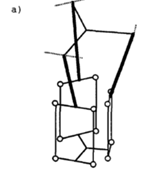
\includegraphics[width=0.3\textwidth]{Main/Chapter4/Images4/Metodo_A_Modelacion_Cinematica_Posicion_9a.png}}
          \subfloat[$\det  \left( J_{x} \right) =0 $]{
         \label{f:Cap4_Metodo_A_Modelacion_Cinematica_Posicion_9b}
            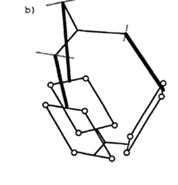
\includegraphics[width=0.3\textwidth]{Main/Chapter4/Images4/Metodo_A_Modelacion_Cinematica_Posicion_9b.png}}
          \subfloat[$ \det  \left( J_{ \theta } \right) =0 $  y $ \det  \left( J_{x} \right) =0 $]{
         \label{f:Cap4_Metodo_A_Modelacion_Cinematica_Posicion_9c}
            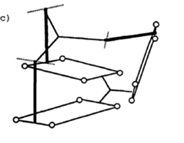
\includegraphics[width=0.3\textwidth]{Main/Chapter4/Images4/Metodo_A_Modelacion_Cinematica_Posicion_9c.png}}
         \caption{Representación de 3 tipos de singularidades de un robot delta \cite{Clavel:31403}}
         \label{f:Cap4_Metodo_A_Modelacion_Cinematica_Posicion_9}
        \end{figure}
        
        \begin{itemize}
	        \item {\fontsize{10pt}{12.0pt}\selectfont Cuando  $\det  \left( J_{ \theta } \right) =0$ . Esto significa que  $\theta _{2i}=0 \lor \pi$ , o \   $\theta _{3i}=0 \lor \pi$  , para  \( i \in \{ 1,2 ,3 \}  \) . En esta situación, los tres pares de barras seguidoras son paralelos. Por tanto, la plataforma móvil tiene 3 grados de libertad, se mueve a lo largo de una superficie esférica y gira sobre el eje perpendicular a la plataforma móvil (figura \eqref{f:Cap4_Metodo_A_Modelacion_Cinematica_Posicion_9a}) .Al mismo tiempo, esta configuración representa el límite del espacio de trabajo, es decir, los puntos más lejanos que puede alcanzar el robot. }

	        \item {\fontsize{10pt}{12.0pt}\selectfont Cuando  $\det  \left( J_{x} \right) =0 $ . Esto significa que    $ \theta _{1i}+  \theta _{2i}=0 \lor \pi$ , o $\theta _{3i}=0 \lor \pi $   , para  \( i \in \{ 1,2 ,3 \}  \) . En esta situación, dos pares de barras seguidoras son paralelas. Los la plataforma móvil tiene 1 grado de libertad, es decir, la plataforma móvil se mueve en una sola dirección (figura \eqref{f:Cap4_Metodo_A_Modelacion_Cinematica_Posicion_9b}).}

	        \item {\fontsize{10pt}{12.0pt}\selectfont Cuando $ \det  \left( J_{ \theta } \right) =0 $  y $ \det  \left( J_{x} \right) =0 $. Esta situación ocurre cuando  $  \theta _{3i}=0 \lor \pi  $  , para  \( i \in \{ 1,2 ,3 \}  \) . En esta situación, dos pares de barras seguidoras están en el mismo plano o dos planos paralelos. La plataforma móvil tiene 1 grado de libertad, es decir, la plataforma móvil gira solamente sobre el eje horizontal (figura \eqref{f:Cap4_Metodo_A_Modelacion_Cinematica_Posicion_9c}).}
\end{itemize}

    
    \newpage
    
    \subsection{Modelación cinemática de aceleración}\label{ma_acel}

    En esta sección se presentan las ecuaciones para determinar la aceleración angular de los actuadores del robot delta. La aceleración angular se determina derivando matricialmente la ecuación \eqref{eq:cap4_eq_26} de la sección \eqref{ma_cvel} llamada modelación cinemática de velocidad para el método A.

    \vspace{-2.5em}

    \begin{align}
    \begin{split}
          \ddot{ \theta }=J_{ \theta }^{-1}\ast \left[ \dot{J}_{x}v_{p}+J_{x}a_{p}-\dot{J}_{ \theta }\dot{ \theta } \right] 
    \end{split}
    \label{eq:cap4_eq_34}
    \end{align}
    
    
    Las matrices en la ecuación \eqref{eq:cap4_eq_34} son: 
        \vspace{-0.5em}
    \begin{multline}
            \left[ \begin{matrix}
        \ddot{ \theta }_{11}~\\
        \ddot{ \theta }_{12}\\
        \ddot{ \theta }_{13}~\\
        \end{matrix}\right] = \left[ \begin{matrix}
        J_{1 \theta }~  &  0  &  0\\
        0  &  J_{2 \theta }~~  &  0\\
        0  &  0  &  J_{3 \theta }~\\
        \end{matrix} \right] ^{-1} \\
    \ast         \left[  \left[ \begin{matrix}
        \dot{J}_{1x}  &  \dot{J}_{1y}  &  \dot{J}_{1z}\\
        \dot{J}_{2x}  &  \dot{J}_{2y}  &  \dot{J}_{2z}\\
        \dot{J}_{3x}  &  \dot{J}_{3y}  &  \dot{J}_{3z}\\
        \end{matrix}\right]   \left[ \begin{matrix}
        v_{px}\\
        v_{py}\\
        v_{pz}\\
        \end{matrix}\right]+\left[ \begin{matrix}
        J_{1x}  &  J_{1y}  &  J_{1z}\\
        J_{2x}  &  J_{2y}  &  J_{2z}\\
        J_{3x}  &  J_{3y}  &  J_{3z}\\
        \end{matrix} \right] \left[ \begin{matrix}
        a_{px}\\
        a_{py}\\
        a_{pz}\\
        \end{matrix}\right] - \left[ \begin{matrix}
        \dot{J}_{1 \theta }~  &  0  &  0\\
        0  &  \dot{J}_{2 \theta }~~  &  0\\
        0  &  0  &  \dot{J}_{3 \theta }~\\
        \end{matrix} \right] \left[ \begin{matrix}
        \dot{ \theta _{11}}~\\
        \dot{ \theta _{12}}\\
        \dot{ \theta _{13}}~\\
        \end{matrix} \right]  \right] ~
        \label{eq:cap4_eq_35}
    \end{multline}
    

    Donde:
    
    \vspace{-1.0em}
    
        \begin{align}
        \dot{J}_{ix}={}& A'_{ix}-B'_{ix}
        \label{eq:cap4_eq_36} \\[0.5cm]
        A'_{ix}={}& cos \phi _{i}\ast \left[  \left[ -\sin  \left(  \theta _{1i}+ \theta _{2i} \right) \ast \left( \dot{ \theta }_{1i}+\dot{ \theta }_{2i} \right) \ast sin  \theta _{3i} \right]  + \left[ \cos  \left(  \theta _{1i}+ \theta _{2i} \right) \ast cos  \theta _{3i}\ast\dot{ \theta }_{3i} \right]  \right]
        \label{eq:cap4_eq_37} \\[0.5cm]
        B'_{ix}={}& sin \phi _{i}\ast \left[ -sin \theta _{3i}\ast\dot{ \theta }_{3i} \right] 
        \label{eq:cap4_eq_38} \\[0.5cm]
        \dot{J}_{iy}={}& A'_{iy}+B'_{iy}
        \label{eq:cap4_eq_39} \\[0.5cm]
        A'_{iy}={}& sin \phi _{i}\ast \left[  \left[ -sin \left(  \theta _{1i}+ \theta _{2i} \right) \ast \left( \dot{ \theta }_{1i}+\dot{ \theta }_{2i} \right) \ast sin~ \theta _{3i} \right] + \left[ \cos  \left(  \theta _{1i}+ \theta _{2i} \right) \ast cos  \theta _{3i}\ast\dot{ \theta }_{3i} \right]  \right]
        \label{eq:cap4_eq_40} \\[0.5cm]
        B'_{iy}={}& cos \phi _{i}\ast \left[ -sin  \theta _{3i}\ast\dot{ \theta }_{3i} \right]
        \label{eq:cap4_eq_41} \\[0.5cm]
        \dot{J}_{iz}={}& \left[ \cos  \left(  \theta _{1i}+ \theta _{2i} \right) \ast \left( \dot{ \theta }_{1i}+\dot{ \theta }_{2i} \right) \ast sin  \theta _{3i} \right] + \left[ sin \left(  \theta _{1i}+ \theta _{2i} \right) \ast cos \theta _{3i}\ast \dot{ \theta }_{3i} \right]
        \label{eq:cap4_eq_42} \\[0.5cm]
        \dot{J}_{i \theta }={}&a \left[ ~ \left[ \cos  \theta _{2i}\ast\dot{ \theta }_{2i}\ast \sin  \theta _{3i} \right] + \left[ \sin  \theta _{2i}\ast cos \theta _{3i}\ast\dot{ \theta }_{3i} \right]  \right]
        \label{eq:cap4_eq_43}
    \end{align}

\newpage

    \begin{align}
        \dot{ \theta }_{3i}={}& \left[ \frac{-1}{\sqrt[]{1- \left( \frac{c_{yi}}{b} \right) ^{2}~}} \right] \ast \left[ \frac{c_{yi}^{'}}{b} \right]
        \label{eq:cap4_eq_44}\\[0.5cm]
        c_{yi}^{'}={}& \left[ -sin \phi _{i}\ast v_{px} + cos \phi _{i}\ast v_{py} \right]
        \label{eq:cap4_eq_45}\\[0.5cm]
       \dot{ \theta }_{2i}={}& \left[ \frac{-1}{\sqrt[]{1- \left(  K \right) ^{2}~}} \right] \ast \left[ K' \right]
        \label{eq:cap4_eq_46}\\[0.5cm]
        K={}& \frac{c_{xi}^{2}+c_{yi}^{2}+c_{zi}^{2}- a^{2}-b^{2}~}{\text{$2ab$ }sin~ \theta _{3i}}
        \label{eq:cap4_eq_47}\\[0.5cm]
       K^{'}={}& \left[ \frac{1}{2ab} \right] \ast \left[ \frac{A_{11}-A_{12}~}{B_{1}} \right]
        \label{eq:cap4_eq_48}\\[0.5cm]
        A_{11}={}& \left[ 2c_{xi}c_{xi}^{'}+2c_{yi}c_{yi}^{'}+2c_{zi}c_{zi}^{'} \right] \ast \left[ sin  \theta _{3i} \right]
        \label{eq:cap4_eq_49}\\[0.5cm]
        A_{12}={}& \left[ c_{xi}^{2}+c_{yi}^{2}+c_{zi}^{2}- a^{2}-b^{2} \right] \ast \left[ cos~ \theta _{3i}\ast\dot{ \theta }_{3i} \right]
        \label{eq:cap4_eq_50}\\[0.5cm]
        B_{1}={}& \left[ \sin  \theta _{3i} \right] ^{2}
        \label{eq:cap4_eq_51}\\[0.5cm]
       c_{xi}^{'}={}& cos \phi _{i}\ast v_{px}+~ sin \phi _{i}\ast v_{py}
        \label{eq:cap4_eq_52}\\[0.5cm]
       c_{zi}^{'}={}& v_{pz}
        \label{eq:cap4_eq_53}
    \end{align}


         \newpage






    \newpage

    
    \subsection{Modelación dinámica}\label{ma_dina}
            La aplicación directa de las leyes de Newton al movimiento de sistemas de partículas es sustituida por una propuesta más general, un método para encontrar las ecuaciones de movimiento para todos los sistemas dinámicos, desarrollado por el matemático Joseph Louis Lagrange. En el anexo \eqref{anexoB} se detalla esta propuesta. Primero se habla de los conceptos básicos hasta llegar a la formulación de Lagrange. Luego se obtienen las ecuaciones de Lagrange partiendo del principio de D’Alembert.  Finalmente se aplican las ecuaciones de Lagrange al robot delta para determinar el torque de cada actuador. Toda la información teórica en esta sección es recopilada del libro
            \cite{INTRO_MECANICA_LAGRAGE}.

        \subsubsection{Teoria de las ecuaciones de Lagrange}

        Se dice que las ligaduras holónomas son empleadas en forma explícita cuando no se utilizan para eliminar las coordenadas dependientes, efectuándose la descripción del sistema de partículas dado con la totalidad (dependientes + independientes) de sus coordenadas. Las ecuaciones de Lagrange para sistemas con ligaduras holónomas usadas de forma explícita se representa en la siguiente formula:
        
        \begin{equation}
             \frac{d}{dt} \left( \frac{ \delta L}{ \delta \dot{q}_{j}} \right) -\frac{ \delta L}{ \delta q_{j}}=Q_{j}^{ \left( lig \right) } \left( q_{j} \right) +Q_{j}^{ \left( NU \right) } \left( q_{j} \right)
             \label{eq:cap4_dina_ma_1}
        \end{equation}
        
        Con  $ j=1,2,3, \ldots , \eta =3N $ 

        Donde:
        \begin{equation}
          Q_{j}^{ \left( lig \right) } \left( q_{j} \right) = \sum _{l=1}^{K^{ \left( h \right) }} \lambda _{l}\frac{ \delta f_{l}^{ \left( h \right) }}{ \delta q_{j}}
             \label{eq:cap4_dina_ma_2}
        \end{equation}

         \( L \)  representa el lagrangiana o lagrangiano:\par
        
        
        \begin{equation}
         L \left( q_{j},\dot{q_{j}},t \right) =T \left( q_{j},\dot{q_{j}},t \right) -V \left( q_{j},\dot{q_{j}},t \right) 
             \label{eq:cap4_dina_ma_3}
        \end{equation}


      Las ecuaciones \eqref{eq:cap4_dina_ma_1} son las ecuaciones de Lagrange para ligaduras holónomas  $f_{i}^{(h)}$ $( q_{i},t) =0$  cuando son usadas en forma explícita. Representan un conjunto de  $\eta =3N$  ecuaciones para el conjunto completo de coordenadas (dependientes + independientes)  $q_{1},q_{2},q_{3},...,q_{\eta=3N}$. Estas ecuaciones, en conjunto con las  $K^{ \left( h \right) }$ ecuaciones de ligadura dadas por $f_{i}^{(h)}$ $( q_{i},t) =0$  forman un sistema de   $ 3N+~K^{ \left( h \right) } $  ecuaciones para  $ 3N+~K^{ \left( h \right) } $  incógnitas,  $ 3N $  coordenadas  $ q_{j} $ y  $ K^{ \left( h \right) } $ multiplicadores de Lagrange  $ \lambda _{l}$ , quedando así determinado dicho sistema de ecuaciones. Aquí las ligaduras entran en forma explícita en los  $ Q_{j}^{ \left( lig \right) }$ dados por la ecuacion \eqref{eq:cap4_dina_ma_2}, que son fuerzas adicionales que actúan sobre el sistema. Debido a que estas fuerzas están relacionadas con las ligaduras se les da el nombre de fuerzas generalizadas de ligadura, las cuales no realizan trabajo virtual como lo requiere la validez del Principio de D’Alembert.


    \newpage
    
    
     $ Q_{j}^{ \left( NU \right) }$ son llamadas comúnmente fuerzas generalizadas, sin embargo, no solo son fuerzas. Estas dependen de la dimensión de las coordenadas generalizadas  $ q_{j}$ que se utiliza en la ecuación de Lagrange :
    
    \begin{enumerate}
    	\item Si $q_{j}$  es una longitud, entonces $Q_{j}^{ \left( NU \right)}$  es una fuerza.
    	\item Si  $q_{j}$  es un ángulo, entonces  $Q_{j}^{ \left( NU \right) }$  es un torque.
        \item Si  $q_{j}$  es una superficie, entonces  $Q_{j}^{ \left( NU \right) }$ es una tensión.
    	\item Si $q_{j}$ es un volumen, entonces es $Q_{j}^{ \left( NU \right) }$ una presión.
    \end{enumerate}

    \newpage


    \subsubsection{Nomenclatura de parámetros geométricos y sistema de referencia global}
    
            \begin{figure}[htb]
                 \centering
                 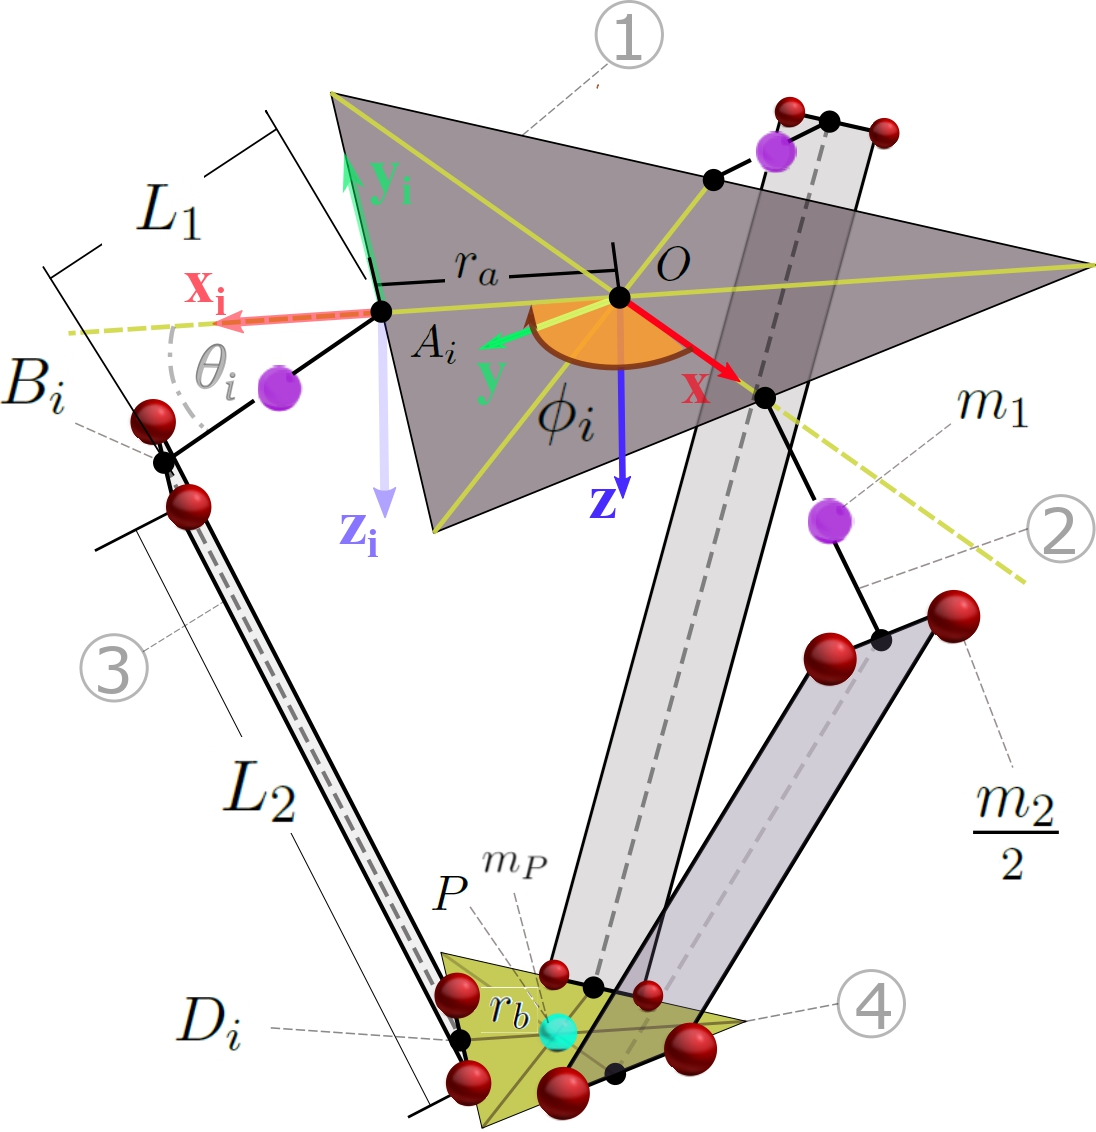
\includegraphics[width=0.77\linewidth]{Main/Chapter4/Images4/DIBUJO23.jpg}
                  \caption{Sistema de referencia local, parámetros geométricos y masas para la solución de la dinámica inversa del método A \cite{Clavel:31403}.}
                  \label{f:Cap4_Metodo_A_dina_1}
            \end{figure}    

En la figura \eqref{f:Cap4_Metodo_A_dina_1} se pueden visualizar 3 cadenas cinemáticas $i\in\{1,2,3\}$ las cuales se componen de 4 partes mecánicas: la base fija, brazos, antebrazos y base móvil. La unión entre la base fija y los brazos representa una junta tipo revoluta accionadas por motores. También se muestra la simplificación de masas para resolver la dinámica del robot delta.

En la tabla \eqref{tab:cap4_tabla_dina_ma_1} muestra la relación entre la numeración en la figura \eqref{f:Cap4_Metodo_A_dina_1} y su nombre.


        \begin{table}[h]
            \centering
            \begin{tabular}{c c}
            \hline
                \textbf{Numero}& \textbf{Descripción} \\ 
            \hline             \hline
             1 & Base fija \\
            \hline
             2 & Brazo \\
            \hline
             3 & Antebazo \\
            \hline
             4 & Base Movil\\
            \hline
            \end{tabular}
            \caption{Relación entre la numeración y piezas mecánicas de la figura  \eqref{f:Cap4_Metodo_A_dina_1}}           \label{tab:cap4_tabla_dina_ma_1}
        \end{table}

    \newpage
   
   En la tabla \eqref{tab:cap4_tabla_dina_ma_2} se presenta la simbología de los sistema de referencia, magnitudes, puntos y ángulos principales para el desarrollo de la dinámica inversa del robot delta.
   
           \begin{table}[h]
            \centering
            \renewcommand{\arraystretch}{1.35}
                \begin{tabular}{c m{11cm}}
            \hline
                \textbf{Simbolo}& \textbf{Descripción} \\ 
            \hline             \hline
             $L_{1}$ &  Longitud brazo\\
            \hline
             $L_{2}$ & Longitud antebrazo \\
            \hline
            $ r_{a}$ &  Radio de circulo inscrito en triangulo de base fija\\
            \hline
             $r_{b}$ & Radio de circulo inscrito en triangulo de base móvil \\
            \hline
            $m_{1}$ & Masa de un brazo posicionada en su centroide \\
            \hline
             $m_{2}$ & Masa de una de las dos barras de los antebrazos, distribuida equitativamente en las extremidades. \\
            \hline
             $m_{P}$ & Masa de la base móvil. \\
            \hline
             $A_{i}$ & Punto de unión entre base fija y brazo para la cadena cinemática $i\in\{1,2,3\}$ \\
            \hline
             $B_{i}$ & Punto de unión entre brazo y antebrazo para la cadena cinemática $i\in\{1,2,3\}$ \\
            \hline
             $D_{i}$ & Punto de unión entre antebrazo y base móvil para la cadena cinemática $i\in\{1,2,3\}$ \\
            \hline
             $P$ & Punto que representa el centroide base móvil\\
            \hline
             $\phi _{i}$ & Ángulo que representa la posición angular de los 3 actuadores sobre el plano de la base fija en relación al sistema de referencia  local para la cadena cinemática $i\in\{1,2,3\}$. \\
            \hline
             $\theta _{i}$ & Ángulo que representa la posición angular de los brazos respecto al eje construido por el punto del origen del sistema de referencia local  y  para la cadena cinemática $i\in\{1,2,3\}$.\\
            \hline
             $O$ – $xyz$ & Sistema de referencia local utilizado para resolver la dinámica del robot delta \\
            \hline
            $A_{i}$ – $x_{i}y_{i}z_{i}$ & Sistema de referencia con origen coincidente en la junta revoluta que una la base fija con los brazos para la cadena cinemática $i\in\{1,2,3\}$ \\
            \hline
             $F_{x},F_{y},F_{z}$ & Fuerzas externas sobre la base móvil\\
            \hline
            \end{tabular}
           \caption{Simbología y descripción de los sistema de referencia, longitudes, puntos y ángulos principales para el desarrollo de la dinámica inversa del método A.}
           \label{tab:cap4_tabla_dina_ma_2}
        \end{table}
   

    \newpage


    \subsubsection{Dinámica inversa}
    
        Un paso importante en el proceso de diseño de un robot es comprender el comportamiento del dispositivo mientras se mueve por su espacio de trabajo o al realizar una tarea específica. Este comportamiento se determina mediante el estudio de la dinámica del mecanismo, donde se pueden determinar las fuerzas que actúan sobre los elementos y los pares requeridos por los actuadores. En consecuencia, cada componente debe optimizarse en dimensiones y material para ser utilizado en los procesos de fabricación. Por lo tanto, es esencial buscar cuáles son los enfoques comunes utilizados para calcular la dinámica del robot. Hay tres enfoques: en primer lugar, la formulación de Newton-Euler, que es un método tradicional basado en las leyes de Newton, pero necesita una gran cantidad de ecuaciones, ya que requiere establecer un número n de ecuaciones para cada elemento con el fin de resolver el sistema. Como resultado, es el método más lento en cuanto a eficiencia computacional. En segundo lugar, el principio de trabajo virtual, que es una derivación del método de Euler y Lagrange utilizando el cálculo de variaciones, se ha utilizado para estudiar la mecánica de los cuerpos deformables. Este enfoque establece que el trabajo total realizado por una fuerza a lo largo de la trayectoria sobre una partícula se puede calcular si esas fuerzas actúan cuando la partícula se mueve del punto A al punto B. Finalmente el tercer enfoque es la formulación lagrangiana, que se basa en variaciones de cálculo, establece que un sistema dinámico puede expresarse en términos de su energía cinética y potencial conduciendo de manera sencilla a la solución del problema. Además, se considera una buena opción para el control en tiempo real de manipuladores paralelos.
    
         Newton estableció los fundamentos de la dinámica donde se deben identificar las fuerzas que producen el cambio para resolver la dinámica de un cuerpo. En su enfoque, se utiliza un diagrama de cuerpo libre para representar todas las fuerzas de cada cuerpo para desarrollar el análisis. Por el contrario, Leibniz, un contemporáneo de Newton, pensó que la acción de una fuerza podría medirse analizando los cambios en la energía potencial y cinética. Más tarde, los métodos variacionales aparecieron formalmente gracias a Lagrange y Hamilton. En este enfoque, la energía, que es una cantidad escalar, facilita el análisis del trabajo realizado en comparación con vectores como la velocidad y la aceleración, que pueden volverse engorrosos en algunos sistemas de coordenadas. La ventaja de utilizar un enfoque lagrangiano es que mientras que en la mecánica vectorial es necesario definir un sistema de coordenadas específico para todos los objetos analizados, en los métodos variacionales no importa si un objeto está en coordenadas cilíndricas y el otro en coordenadas esféricas. Los detalles no son importantes siempre que puedan expresarse en términos de coordenadas que tienen tres coordenadas que se refieren al centro de masa del cuerpo y tres coordenadas a la orientación específica del cuerpo en el espacio.

    \newpage
            
        Las ecuaciones de Lagrange para el robot delta en este trabajo se definen a partir de 6 coordenadas generalizadas y 3 restricciones holónomas de forma explícita. Por lo tanto, la modelación dinámica se resume en las siguientes ecuaciones:
            
        \begin{equation}
         \frac{d}{dt} \left( \frac{ \delta L}{ \delta \dot{q}_{j}} \right) -\frac{ \delta L}{ \delta q_{j}}=Q_{j}^{ \left( lig \right) } \left( q_{j} \right) +Q_{j}^{ \left( NU \right) } \left( q_{j} \right)
             \label{eq:cap4_dina_ma_4}
        \end{equation}
        
        \begin{equation}
         Q_{j}^{ \left( lig \right) } \left( q_{j} \right) = \sum _{l=1}^{K^{ \left( h \right) }} \lambda _{l}\frac{ \delta f_{l}^{ \left( h \right) }}{ \delta q_{j}}
             \label{eq:cap4_dina_ma_5}
        \end{equation}
        
         \begin{equation}
          L \left( q_{j},\dot{q_{j}},t \right) =T \left( q_{j},\dot{q_{j}},t \right) -V \left( q_{j},\dot{q_{j}},t \right)
        \label{eq:cap4_dina_ma_6}
        \end{equation}
        
        \vspace{-0.8cm}
        \begin{multline}
         T= \left[ \frac{1}{2}m_{P} \left( \dot{X}_{p}^{2}+\dot{Y}_{p}^{2}+\dot{Z}_{p}^{2} \right)  \right] + \left[  \left( \frac{1}{6}m_{1}L_{1}^{2} \right) \ast \sum _{i=1}^{3} \left( \dot{ \theta }_{i} \right) ^{2} \right] + \\
          \left( \frac{m_{2}}{2} \right) \ast \left[  \sum _{i=1}^{3} \left( \dot{X}_{p}^{2}+\dot{Y}_{p}^{2}+\dot{Z}_{p}^{2} \right) + \left( L_{1}^{2}\dot{ \theta }_{i}^{2} \right)  \right]
        \label{eq:cap4_dina_ma_7}
        \end{multline}
        \vspace{-0.8cm}
 
        \begin{equation}
         V=- \left[ m_{p}gZ_{p} \right] - \left[ \frac{1}{2}m_{1}gL_{1} \sum _{i=1}^{3}\sin  \theta _{i} \right] - \left[ m_{2}gL_{1} \sum _{i=1}^{3}\sin  \theta _{i} \right] - \left[ 3m_{2}gZ_{p} \right]
        \label{eq:cap4_dina_ma_8}
        \end{equation}
        
        \begin{equation}
         q_{j} \in \{X_{p},Y_{p},Z_{p}, \theta _{1}, \theta _{2}, \theta _{3} \}
        \label{eq:cap4_dina_ma_9}
        \end{equation}
        
        \begin{equation}
         K^{ \left( h \right) }=3
        \label{eq:cap4_dina_ma_10}
        \end{equation}

        \vspace{-1cm}
        \begin{multline}
             f_{i}^{ \left( h \right) } \left(  \theta _{i}, \phi _{i} \right) = \left( X_{P}-L_{1}\cos  \theta _{i}\cos  \phi _{i}- rcos \phi _{i} \right) ^{2}+ \\ 
             \left( Y_{P}-L_{1}\cos  \theta _{i}\sin  \phi _{i}- rsin \phi _{i} \right) ^{2}+ \left( Z_{P}-L_{1}\sin  \theta _{i} \right) ^{2}-L_{2}^{2}
        \label{eq:cap4_dina_ma_11}
        \end{multline}
        
    
        Donde  $L$  es el lagrangiano, $T$ es la energía cinética total,  $ V$  es la energía potencial,  $ q_{j}$  es la j-ésima coordenada generalizada,  $ \left( X_{p},~Y_{p},~Z_{p} \right)$  representan las coordenadas del centroide de la plataforma móvil, $\left(  \theta _{1}, \theta _{2}, \theta _{3} \right) $  es la posición angular de los motores, $Q_{j}^{ \left( NU \right) } $  son fuerzas externas generalizadas (no potencial), $\lambda _{l}$ es el multiplicador de Lagrange , $ K^{ \left( h \right) }$ cantidad de restricciones holónomas y  $f_{l}^{ \left( h \right) }$  son la ecuación de restricción holónomas de forma explícita. Las fuerzas de fricción no son restricciones a pesar de que juegan un papel importante en el análisis de la dinámica, por lo que pueden tratarse por separado. Una vez que se introduce la ecuación de Lagrange para el movimiento y se establecen los parámetros necesarios para su análisis, es posible calcular el torque en los actuadores de un robot delta bajo una trayectoria específica.
    
    
    
    
    
    \newpage
    
    
    Se sabe que, si en el las ecuaciones de Lagrange la coordenada generalizada  $  q_{j} $   es un ángulo, entonces  $  Q_{j}^{ \left( NU \right) } \left( q_{j} \right)  $   representa un torque. Por lo tanto, para determinar el torque necesario en los motores para realizar una determinada trayectoria de la base móvil, se resuelven las ecuaciones de Lagrange con las coordenadas generalizadas  $ q_{j}= \left[  \theta _{1}, \theta _{2}, \theta _{3} \right]  $  . La ecuación que determina los torques de los motores $i\in\{1,2,3\}$  es:
    
    \begin{multline}
    \tau_{i}= \left( \frac{1}{3}m_{1}+m_{2} \right) L_{1}^{2}\ddot{ \theta }_{i}- \left( \frac{1}{2}m_{1}+m_{2} \right) gL_{1}\cos  \theta _{i}\\
    -2 \lambda _{i}L_{1} \left[  \left( X_{P}\cos  \phi _{i}+Y_{P}\sin  \phi _{i}- r \right) \sin  \theta _{i}-Z_{P}\cos  \theta _{i} \right] 
    \label{eq:cap4_dina_ma_15}
    \end{multline}

    Donde los coeficientes de Lagrange $  \lambda _{i} $ se determinan resolviendo el sistema de ecuaciones a partir de:
    
    \begin{equation}
     \left( m_{p}+3m_{2} \right) \ddot{X}_{p}-2 \sum _{l=i=1}^{3} \lambda _{l} \left( X_{P}- rcos \phi _{i}-L_{1}\cos  \theta _{i}\cos  \phi _{i} \right) =F_{px} 
        \label{eq:cap4_dina_ma_12}
    \end{equation}
    
    \begin{equation}
     \left( m_{P}+3m_{2} \right) \ddot{Y}_{p}-2 \sum _{l=i=1}^{3} \lambda _{l} \left( Y_{P}- rsin \phi _{i}-L_{1}\cos  \theta _{i}\sin  \phi _{i} \right) =F_{py} 
        \label{eq:cap4_dina_ma_13}
    \end{equation}

    \begin{equation}
      \left( m_{P}+3m_{2} \right) \ddot{Z}_{p}-2 \sum _{l=i=1}^{3} \lambda _{l} \left( Z_{P}-L_{1}\sin  \theta _{i} \right) - \left( m_{p}+3m_{2} \right) g=F_{pz} 
        \label{eq:cap4_dina_ma_14}
    \end{equation}

    El término $ \left( F_{px},F_{py},F_{pz} \right)$ son las fuerzas externas que se aplican a la base móvil y   $r=r_{a}-r_{b}$.







    \newpage


\section{Método B}

    \subsection{Modulación cinemática de la posición}\label{MB_MP}
    
            Con el objetivo de modelar la cinemática del robot delta, en esta sección se implementan las ideas expuestas en la tesis doctoral  \cite{Path_Planning_and_Trajectory_Optimization}, que aborda en uno de sus capítulos la problemática de cinemática directa e inversa.
    
        \subsubsection{Nomenclatura de parámetros geométricos y sistema de referencia local}

            En la figura \eqref{f:Cap4_Metodo_B_Modelacion_Cinematica_Posicion_1} se presenta el sistema de referencia local, las partes mecánicas y la nomenclatura de los parámetros del robot delta simplificado para resolver el problema de cinemática.

            \begin{figure}[htb]
                 \centering
                 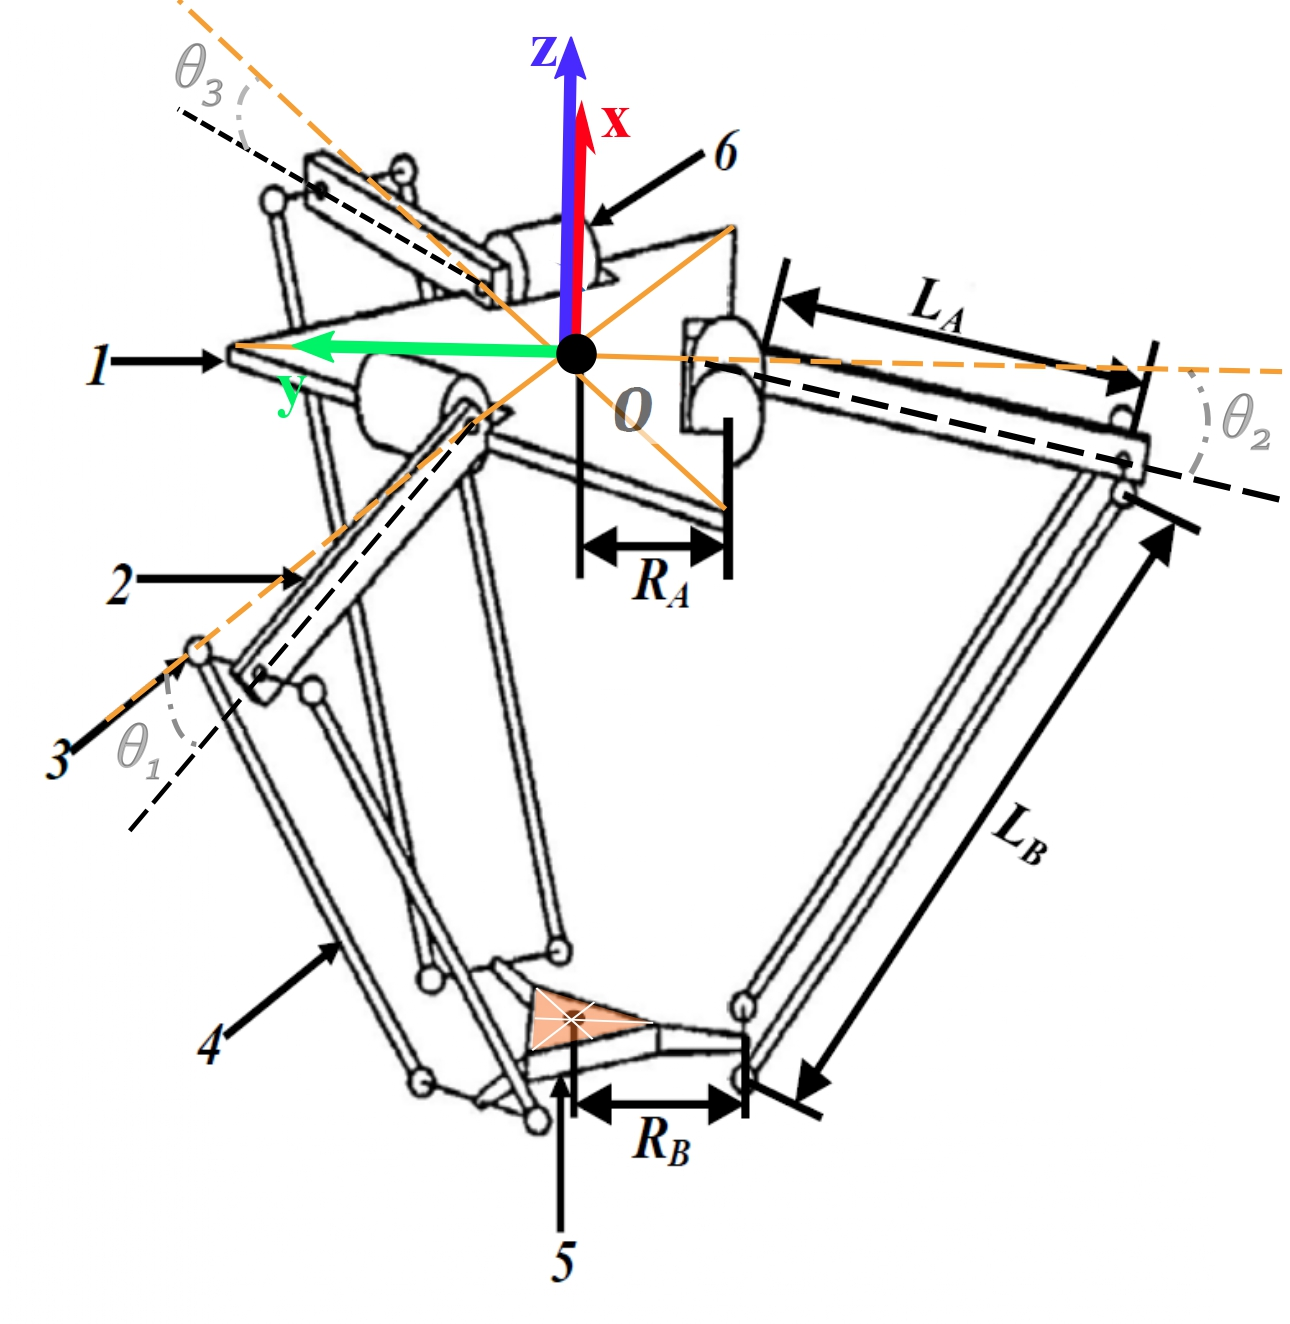
\includegraphics[width=0.53\linewidth]{Main/Chapter4/Images4/DIBUJO24.jpg}
                  \caption{Sistema de referencia local para la cinemática del método B \cite{Path_Planning_and_Trajectory_Optimization}.}
                  \label{f:Cap4_Metodo_B_Modelacion_Cinematica_Posicion_1}
            \end{figure}        
        
        
        La tabla \eqref{tab:cap4_tabla_11} muestra la relación entre la numeración en la figura \eqref{f:Cap4_Metodo_B_Modelacion_Cinematica_Posicion_1} y su nombre:
        \begin{table}[h]
            \centering
            \begin{tabular}{c c}
            \hline
                \textbf{Numero}& \textbf{Nombre} \\ 
            \hline             \hline
             1 & Base Fija \\
            \hline
             2 & Brazo \\
            \hline
             3 & Junta esférica \\
            \hline
             4 & Antebrazo\\
            \hline
             5 & Efector final \\
             \hline
             6 & Actuador \\
             \hline
            \end{tabular}
           \caption{Nombres de partes mecánicas del robot delta del método B.}
           \label{tab:cap4_tabla_11}
        \end{table}
        
        
        \newpage

        Antes de empezar los cálculos de cinemática, es mejor explicar algunos términos que se utilizan ampliamente en la formulación cinemática.
        

            \begin{figure}[htb]
                 \centering
                 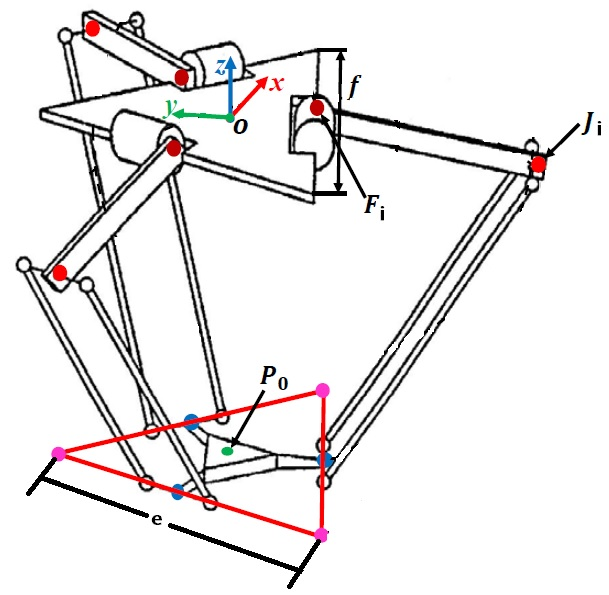
\includegraphics[width=0.52\linewidth]{Main/Chapter4/Images4/DIBUJO25.jpg}
                  \caption{Principales parámetros geométricos y puntos para la solución de la cinemática
del método B \cite{Path_Planning_and_Trajectory_Optimization}.}
                  \label{f:Cap4_Metodo_B_Modelacion_Cinematica_Posicion_2}
            \end{figure}        
        
        
        
        Los parámetros necesarios para resolver la cinemática del robot delta se presentan en las figuras  \eqref{f:Cap4_Metodo_B_Modelacion_Cinematica_Posicion_1} , \eqref{f:Cap4_Metodo_B_Modelacion_Cinematica_Posicion_2} y la  tabla \eqref{tab:cap4_tabla_12}:
        
        \begingroup
            \renewcommand{\arraystretch}{1.3}
            \begin{table}[H]
            \centering
            \begin{tabular}{c m{12cm}}
               \hline
               \textbf{Parametro}  & \multicolumn{1}{c}{\textbf{Descripción}}  \\
               \hline           \hline            
             $L_A$ & Largo del brazo \\
            \hline
             $L_B$ & Largo del antebrazo \\
            \hline
             $R_A$ & Distancia entre el centro de la base fija y la junta revoluta o actuador \\
            \hline
             $R_B$ & Distancia entre el centro del efector a la junta que lo une con el antebrazo\\
            \hline
             $f$ & Longitud de un lado del triángulo equilátero inscribe el círculo formado por los puntos $F'_1$, $F'_2$ y $F'_3$ (base fija)\\
            \hline
             $e$ & Longitud de un lado del equilátero triángulo inscribe el círculo formado por los puntos $P'_1$, $P'_2$ y $P'_3$ (efector final)\\
            \hline
             $\theta_i$ & Angulo de los actuadores\\
            \hline
             $J_i$ & Punto de la junta esférica que conecta los brazos con el antebrazo\\
            \hline            
             $F_i$ & Punto de la posición de los actuadores\\
            \hline  
             $P_0$ & Posición del final efector en el espacio cartesiano con respecto al sistema de coordenadas con origen $O$ en el centroide de la base fija\\
            \hline            
            \end{tabular}
            \caption{Principales parámetros geométricos y puntos para la solución de la cinemática del método B.}
           \label{tab:cap4_tabla_12}
        \end{table}
        \endgroup     
        
        
        \newpage
    
        La definición de los vectores utilizados para la formulación de la solución de cinemática del robot paralelo delta se muestra en la figura \eqref{f:Cap4_Metodo_B_Modelacion_Cinematica_Posicion_33} y en la tabla \eqref{tab:cap4_tabla_1332}. 
    
            \begin{figure}[htb]
                 \centering
                 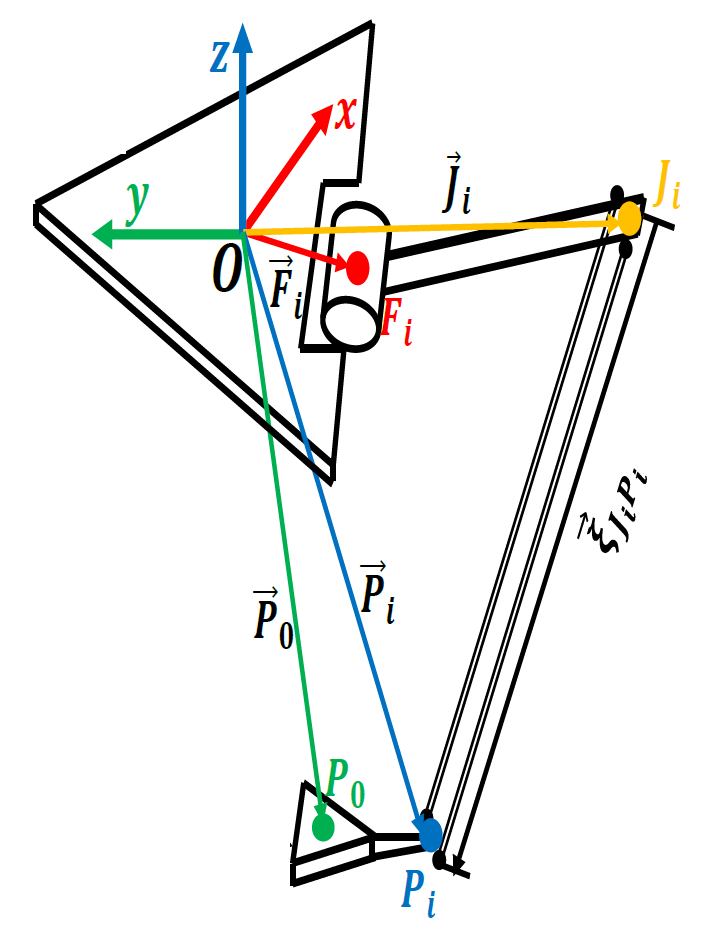
\includegraphics[width=0.55\linewidth]{Main/Chapter4/Images4/DIBUJO26.png}
                  \caption{Vectorización para la solución de cinemática del método B  \cite{Path_Planning_and_Trajectory_Optimization}.}
                  \label{f:Cap4_Metodo_B_Modelacion_Cinematica_Posicion_33}
            \end{figure} 
    
            \begingroup
            \renewcommand{\arraystretch}{1.5}
            \begin{table}[H]
            \centering
            \begin{tabular}{c m{12cm}}
               \hline
               \textbf{Parámetro}  & \multicolumn{1}{c}{\textbf{Descripción}}  \\
               \hline           \hline            
             $\overrightarrow{{P}_{0}}$ & Vector con punto inicial en el centro de la base fija y con extremo en el centro del efector final \\
            \hline
             $\overrightarrow{{P}_{i}}$ & Vector que inicia en el centro de la base fija y su extremo se encuentra en la junta esférica que conecta el efector con el antebrazo $i\in\{1,2,3\}$. \\
            \hline
             $\overrightarrow{{J}_{i}}$ & Vector que inicia en el centro de la base fija y su extremo se encuentra en la junta esférica que conecta el brazo con el antebrazo $i\in\{1,2,3\}$. \\
            \hline
             $\overrightarrow{{F}_{i}}$ & Vector que inicia en el centro de la base fija y su extremo se encuentra en la posición de los motores o actuadores $i\in\{1,2,3\}$ \\
            \hline
             $\overrightarrow{{\xi}_{F_iJ_i}}$ & Vector que inicia en la junta esférica que conecta el brazo con el antebrazo y su extremo se encuentra en la junta esférica que conecta el efector con el antebrazo $i\in\{1,2,3\}$.Este vector es una representación de los antebrazos.
 \\
            \hline
            \end{tabular}
            \caption{Vectorización para la solución de cinemática del método B}
           \label{tab:cap4_tabla_1332}
        \end{table}
        \endgroup     
        
        \newpage


\subsubsection{Cinemática directa}\label{mb_cd}
        
        En\ la cinemática directa se calcula la posición del efector final del manipulador robótico a partir de la información dada de los ángulos en los actuadores.


        \begin{equation}
            \theta _{1},~ \theta _{2}, \theta _{3}~~~ \rightarrow ~  {P_{0}} \left( P_{0x},P_{0y},P_{0z} \right)
        \label{eq:cap4_MB_1}
        \end{equation}

        El método de solución de la cinemática directa en esta sección es el mismo que el empleado para el método A. Lo único que cambia es la nomenclatura de los parámetros y el orden de numeración de los ángulos de los actuadores (figura \eqref{f:cap4_mb_cineposdirect}).
        
        Como los ángulos   $\theta_1,\theta_2,\theta_3$  se conocen en el problema de cinemática directa, las coordenadas de los puntos $J_1,J_2,J_3$   se pueden encontrar fácilmente. Los antebrazos   $\overline{J_1P_1},\overline{J_2P_2},\overline{J_3P_3}$   pueden girar libremente alrededor de los puntos $J_1,J_2,J_3$   respectivamente. A fin de calcular la cinemática directa, los puntos  $J_1,J_2,J_3$   se trasladan a  $J'_1,J'_2,J'_3$ , utilizando los vectores de traslación $\overrightarrow{\xi_{P_1 P_0}},\overrightarrow{\xi_{P_2P_0}},\overrightarrow{\xi_{P_3 P_0}}$    respectivamente, como se muestra en la figura \eqref{f:Cap4_Metodo_B_Modelacion_Cinematica_Posicion_3} (vectores color amarillo).
        
            \begin{figure}[htb]
                 \centering
               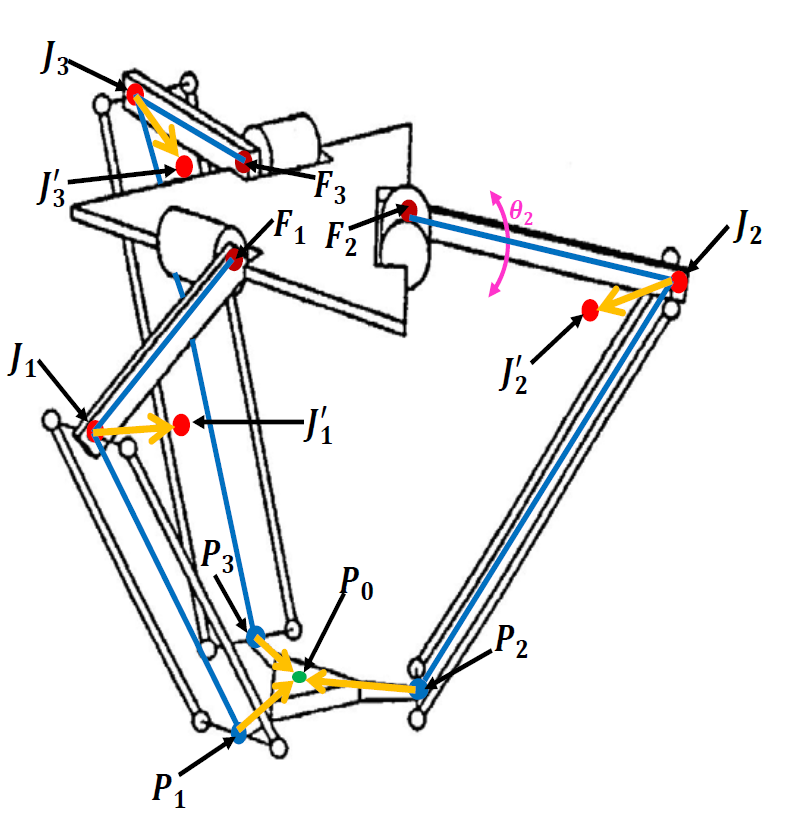
\includegraphics[width=0.7\linewidth]{Main/Chapter4/Images4/DIBUJO28.png}
                  \caption{Traslación de los vectores que representan los antebrazos para crear un sistema de ecuaciones y determinar la cinemática directa del método B \cite{Path_Planning_and_Trajectory_Optimization}.}
                  \label{f:Cap4_Metodo_B_Modelacion_Cinematica_Posicion_3}
            \end{figure}        

        Como resultado de esta traslación se producen tres esferas con radio $L_B$ y centro en los puntos $J'_1,J'_2,J'_3$  que se cruzan en el punto $P_0$.




    \newpage


        
    Resumiendo, al igual que metodo A, el resultado de las traslaciones de las 3 esferas con centros en las juntas esféricas  \( J_{1},~J_{2},J_{3} \)  producen tres nuevas esferas con radio  \( L_{B} \)  y centro en los puntos  \( J'_{1},~J'_{2},J'_{3} \)   que se cruzan en el punto  \( P_{0} \) . Las coordenadas del vector  \( \overrightarrow{P_{0}}=  \left[ P_{0x},P_{0y},P_{0z} \right] ^{T} \)  se pueden obtener resolviendo las tres ecuaciones que representan las nuevas esferas en el espacio cartesiano simultáneamente. Las ecuaciones son:
    
        \begin{equation}
            \left( P_{0x}-J'_{1x} \right) ^{2}+ \left( P_{0y}-J'_{1y} \right) ^{2}+ \left( P_{0z}-J'_{1z} \right) ^{2}=L_{B}^{2}
        \label{eq:cap4_MB_21}
        \end{equation}
        \begin{equation}
            \left( P_{0x}-J'_{2x} \right) ^{2}+ \left( P_{0y}-J'_{2y} \right) ^{2}+ \left( P_{0z}-J'_{2z} \right) ^{2}=L_{B}^{2}
        \label{eq:cap4_MB_22}
        \end{equation}    
        \begin{equation}
            \left( P_{0x}-J'_{3x} \right) ^{2}+ \left( P_{0y}-J'_{3y} \right) ^{2}+ \left( P_{0z}-J'_{3z} \right) ^{2}=L_{B}^{2}
        \label{eq:cap4_MB_23}
        \end{equation}            
    Por lo tanto, se dispone de un sistema de ecuaciones con 3 ecuaciones y con 3 incógnitas \( P_{0x},P_{0y},P_{0z} \) .  
    
    Para la calcular los centros \( J'_{1},~J'_{2},J'_{3} \)  primero se miden las magnitudes de otros vectores que son fundamentales para identificar de mejor forma estos puntos en el espacio y facilitar su cálculo. En las figuras \eqref{f:cap4_mb_cineposdirect} y \eqref{f:Cinematica_Posicion_4B} se muestra la vista superior del robot paralelo delta. Desde esta vista, se puede calcular la magnitud de la traslación de  $J_i$ a  $J'_i$  gracias a que la geometría del efector final es un triangulo equilátero con lados definidos $e$. Esta geometría básica también permite encontrar la distancia desde el centro de la base fija y los actuadores..
    
            \begin{figure}[htb]
                 \centering
               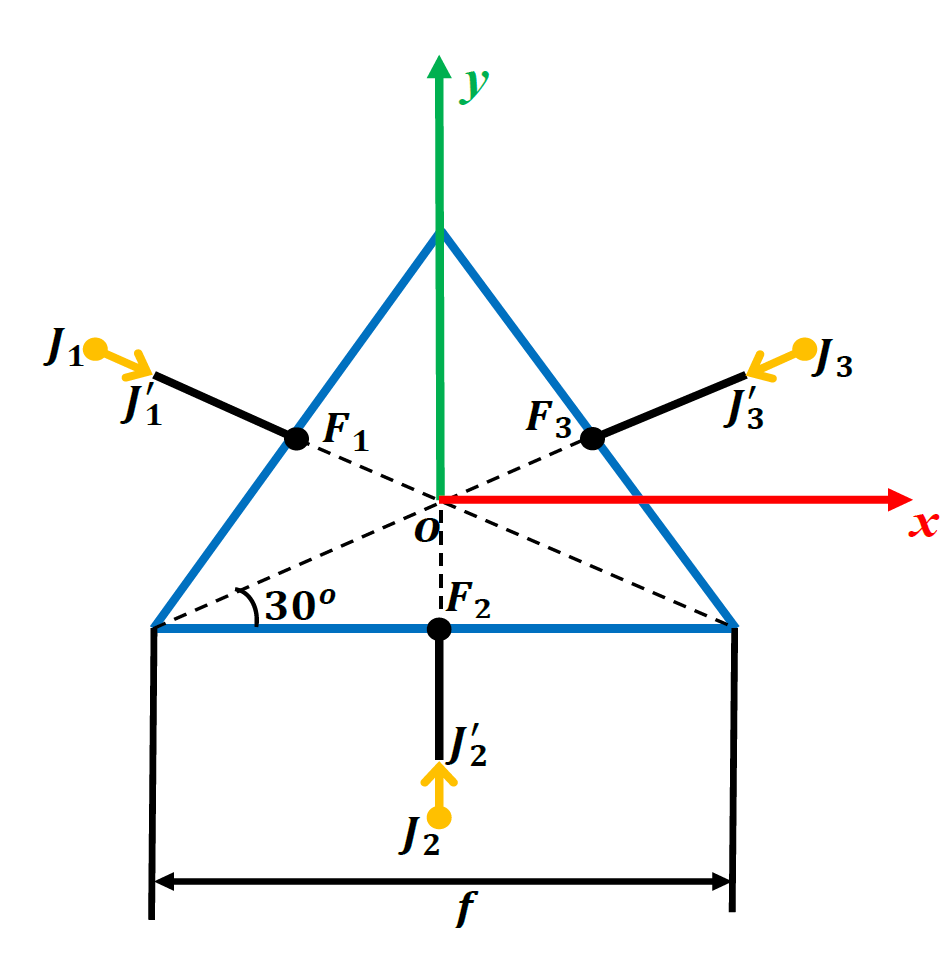
\includegraphics[width=0.45\linewidth]{Main/Chapter4/Images4/DIBUJO29.png}
               \caption{Vista frontal  de la base fija \cite{Path_Planning_and_Trajectory_Optimization}.}
               \label{f:cap4_mb_cineposdirect}
            \end{figure}
            
    \begin{equation}
        \Vert \overrightarrow{\xi_{OF_i}} \Vert=\frac{f}{2}\tan(30)=\frac{f}{2\sqrt{3}} , i \in \{1,2,3\}
    \end{equation}
    \begin{equation}
        \Vert \overrightarrow{\xi_{J_iJ'_i}} \Vert=\frac{e}{2}\tan(30)=\frac{e}{2\sqrt{3}} , i \in \{1,2,3\}
    \end{equation}
    
        \newpage

    El movimiento de los brazos está restringido por una junta tipo revoluta, por ende, es fácil calcular la distancia entre el punto $F_i$ y la proyección del punto $J_i$ en el plano que contiene a la base fija:
    \begin{equation}
        \Vert \overrightarrow{\xi_{F_iJ_i}} \Vert=L_a           \cos(\theta_i) , i \in \{1,2,3\}
    \end{equation}
    
    Según las ecuaciones \eqref{eq:cap4_MB_22}, \eqref{eq:cap4_MB_23} y \eqref{eq:cap4_MB_24}, se forman tres esferas con centros en los puntos \( J'_{1},~J'_{2},J'_{3} \). Las coordenadas de los centros de las esferas se pueden calcular utilizando los vectores de traslación antes mencionados. Las coordenadas de los puntos \( J'_{1},~J'_{2},J'_{3} \) se dan en las ecuaciones \eqref{eq:cap4_MB_3}, \eqref{eq:cap4_MB_4} y \eqref{eq:cap4_MB_5} respectivamente:

  
          \begin{equation}
                \overrightarrow{J'_{1}}= \left [\left( \frac{(f-e)}{2\sqrt{3}}+{L}_{A}\cos(\theta_1)\right) \cos(30^\circ), \left(\frac{(f-e)}{2\sqrt{3}} + {L}_{A}\cos(\theta_1)\right) \sin(30^\circ), -L_{A}\sin(\theta_1)\right]
        \label{eq:cap4_MB_3}
        \end{equation}    
        
        \begin{equation}
                \overrightarrow{J'_{2}}= \left [  0,-\frac{(f-e)}{2\sqrt{3}}-L_{A}\cos(\theta_2),-L_{A}\sin(\theta_2)\right]
        \label{eq:cap4_MB_4}
        \end{equation}    
        
        \begin{equation}
                \overrightarrow{J'_{3}}= \left [\left( \frac{(f-e)}{2\sqrt{3}}+{L}_{A}\cos(\theta_3)\right) \cos(30^\circ), \left(\frac{(f-e)}{2\sqrt{3}} + {L}_{A}\cos(\theta_3)\right) \sin(30^\circ), -L_{A}\sin(\theta_3)\right]
        \label{eq:cap4_MB_5}
        \end{equation}    
  
      Después de calcular todos los vectores de traslación y las coordenadas de los centros de las esferas, el sistema de ecuaciones  \eqref{eq:cap4_MB_22}, \eqref{eq:cap4_MB_23} y \eqref{eq:cap4_MB_24} se puede resolver para obtener la posición del efector final \( P_{0x},P_{0y},P_{0z} \) .El método algebraico para resolver el sistema de ecuaciones, en otras palabras, la intersección de las 3 esferas trasladadas, es el mismo que en el método A, específicamente el sistema de ecuaciones de la ecuación \eqref{eq:cap4_eq_2}.
  
 \newpage
        
        
{\hypersetup{colorlinks=true,        
    linkcolor=blue,         
    filecolor=magenta,       
    urlcolor=russet,           
    citecolor=blue}
    
\subsubsection{Cinemática inversa}\label{mb_ci}

      En la cinemática inversa, se calculan los ángulos de los actuadores gracias a la posición dada de efector final en el espacio cartesiano. 
      
        \begin{equation}
              P_{0} \left( P_{0x},P_{0y},P_{0z} \right) ~~ \rightarrow    \theta _{1},~ \theta _{2}, \theta _{3} 
        \label{eq:cap4_MB_6}
        \end{equation}\par      
      
        El método de solución de la cinemática inversa en esta sección es el mismo que el empleado para el método A. Lo único que cambia es la nomenclatura de los parámetros y el orden de numeración de los ángulos de los actuadores (figura \eqref{f:Cinematica_Posicion_4}).
  
           \begin{figure}[htb]
             \centering
            \subfloat[Intersección de círculos en punto $J_i$]{
                      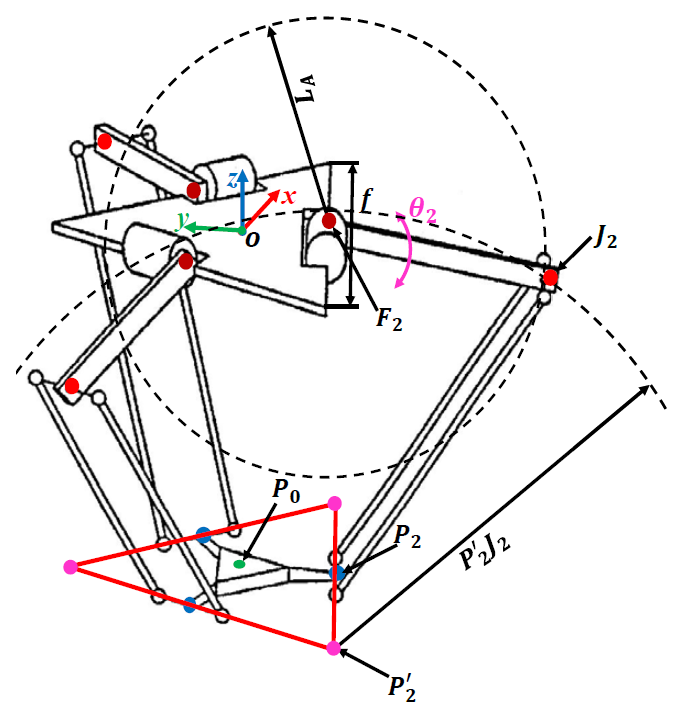
\includegraphics[width=0.52\textwidth]{Main/Chapter4/Images4/DIBUJO27.png}
                        \label{f:Cinematica_Posicion_4a}}
            \subfloat[Vista frontal efector final]{
                      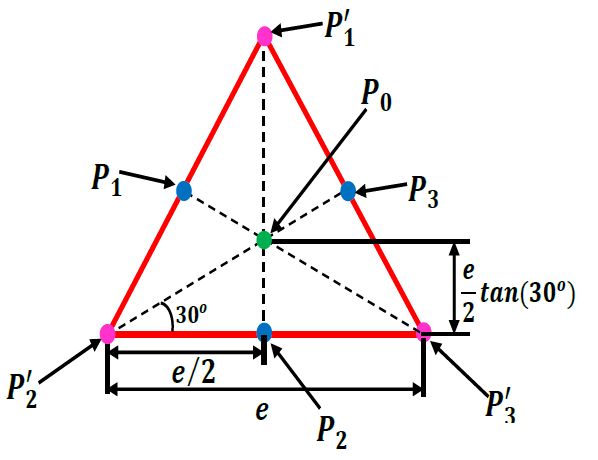
\includegraphics[width=0.4\textwidth]{Main/Chapter4/Images4/DIBUJO30.png}
                        \label{f:Cinematica_Posicion_4B}}
            \caption{Solución de la cinemática directa de posición del método B \cite{Path_Planning_and_Trajectory_Optimization}.}
            \label{f:Cinematica_Posicion_4}
        \end{figure}
  
      Primero se empieza por calcular en ángulo $\theta_2$. Se trabaja sobre el marco de referencia $YZ$, ya que el brazo  \overline{\( F_{2}J_{2}  \)} solo puede moverse en ese plano como se muestra en la figura \eqref{f:Cinematica_Posicion_4a}. Desde la figura \eqref{f:Cinematica_Posicion_4B} se desprenden las coordenadas de punto $F_2=\left[0,\frac{-f}{(2\sqrt{3})},0\right]$. Sobre el plano $ YZ $ se proyecta el antebrazo para obtener una segunda restricción geométrica relacionada con la junta  \( J_{2} \) . En consecuencia, la posición de la junta esférica  \( J_{2} \)  está restringida por 2 circunferencias en el plano $YZ$. Se dibuja el primer círculo con centro  \( F_{2} \)  y radio  \( L_{A} \) . El segundo círculo se dibuja con el centro en el punto  \( P'_{2} \)  y radio  \( \sqrt[]{L_{B}^{2}-P_{0x}^{2}} \), donde el punto $P'_{2}=\left[0,P_{0y}-\frac{e}{2\sqrt{3}},P_{0z}\right]^T$ es la proyección del punto $P_{2}=\left[P_{0x},P_{0y}-\frac{e}{2\sqrt{3}},P_{0z}\right]^T$ sobre plano $YZ$ y el radio de la circunferencia es calculado de la expresión  $\Vert \overrightarrow{\xi}_{P'_2J_2} \Vert = \sqrt{\Vert \overrightarrow{\xi}_{P_2J_2}\Vert^2-\Vert \overrightarrow{\xi}_{P'_2P_2}\Vert^2 }=\sqrt[]{L_{B}^{2}-P_{0x}^{2}}$       como se aprecia en la figura \eqref{f:f:Cap4_Metodo_B_Modelacion_Cinematica_Posicion_44}.
      
     \newpage

            \begin{figure}[htb]
                 \centering
               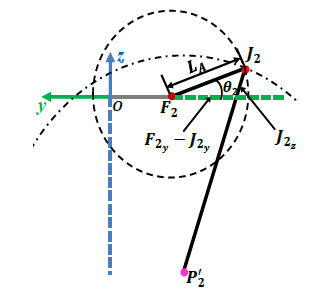
\includegraphics[width=0.7\linewidth]{Main/Chapter4/Images4/Metodo_B_Modelacion_Cinematica_Posicion_4b.png}
               \caption{Proyección del punto $P_2$ sobre el plano YZ \cite{Path_Planning_and_Trajectory_Optimization}.}
               \label{f:f:Cap4_Metodo_B_Modelacion_Cinematica_Posicion_44}
            \end{figure}
            
      La ecuación general de la circunferencia de las ecuaciones \eqref{eq:cap4_MB_7} y \eqref{eq:cap4_MB_8} representan los círculos con radio  \( L_{A} \)  y  \( \sqrt[]{L_{B}^{2}-P_{0x}^{2}} \)  respectivamente, como se muestra en la figura \eqref{f:f:Cap4_Metodo_B_Modelacion_Cinematica_Posicion_44}.
  
  
        \begin{equation*}
              (J_{2y}-F_{2y})^2 + (J_{2z}-F_{2z})^2=  L_{A}^{2}
        \end{equation*}
        \begin{equation}
              \Rightarrow  \left (J_{2y} + \frac{f}{2\sqrt{3}}\right)^2 + J_{2z}^{2}= L_{A}^{2}
        \label{eq:cap4_MB_7}
        \end{equation}     

        \begin{equation*}
              (J_{2y}-{P'}_{2y})^2 + (J_{2z}-{P'}_{2z})^2= L_{B}^{2} -P_{0z}^2 
        \end{equation*}          
        \begin{equation}
             \Rightarrow   \left (J_{2y} - P_{0y}+ \frac{e}{2\sqrt{3}}\right)^2 + ({J}_{2z}-{P}_{0z}) = L_{B}^{2} -P_{0z}^2
        \label{eq:cap4_MB_8}
        \end{equation}  
    
    
        El valor de  \( J_{2y} \)  y  \( J_{2z} \)  se puede calcular resolviendo simultáneamente la ecuación \eqref{eq:cap4_MB_7} y \eqref{eq:cap4_MB_8} al igual que en el método A. Todas las demás parámetros en este sistema de ecuaciones se asumen como conocidos o se obtienen a partir de la estructura geométrica del robot paralelo delta. Una vez que se conocen estos valores, se puede usar trigonometría simple para calcular el  \(  \theta _{2} \)  como se indica en la siguiente ecuación:
        
        \begin{equation} 
            \theta_2=\tan^{-1} \left(\frac{J_{2z}}{{F}_{2y}-{J}_{2y}}\right)
        \label{eq:cap4_MB_9}
        \end{equation}  
        \newpage

        La estructura simétrica del robot paralelo delta da la ventaja de calcular los ángulos  \(  \theta _{1} \)  y  \(  \theta _{3} \)  faltantes aplicando el mismo procedimiento para el ángulo \(  \theta _{2} \) . Para ello, se rotar el marco de referencia local en un ángulo de 120º en sentido antihorario y horario para  \(  \theta _{3} \) y  \(  \theta _{1} \) respectivamente.   
           
        \begin{figure}[htb]
                 \centering
               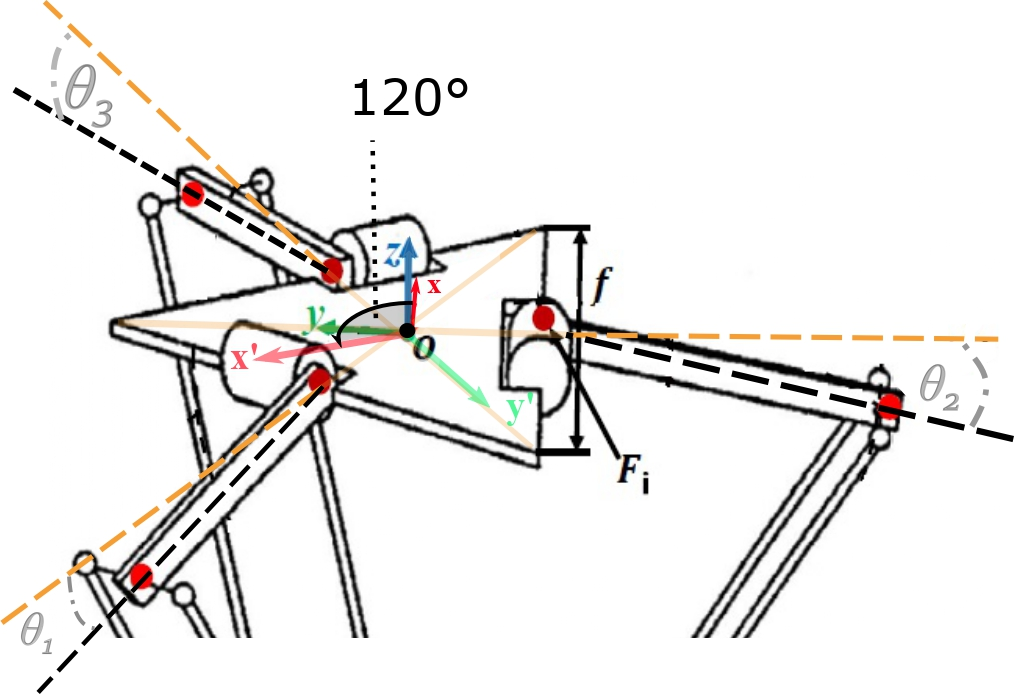
\includegraphics[width=1\linewidth]{Main/Chapter4/Images4/DIBUJO32.jpg}
               \caption{Rotación del sistema de referencia local para la solución de la cinemática inversa del método B \cite{Path_Planning_and_Trajectory_Optimization}.}
               \label{f:f:Cap4_Metodo_B_Modelacion_Cinematica_Posicion_444}
            \end{figure}
        \newpage

\subsection{Modelación cinemática de la velocidad}\label{mb_cvel}
    
        Con el objetivo de modelar la cinemática de velocidad del robot delta, en esta sección se implementa las ideas expuestas en el paper \cite{Path_Planning_and_Trajectory_Optimization},  con los mismos parámetros, jerga y nomenclatura de la seccion  \eqref{MB_MP}
        La base de la modelacion cinematica de velocidad es determinar la matriz jacobiana  \( J \) . Esta juega un papel importante en el modelo dinámico del manipulador robótico como se aprecia en secciones posteriores.\par
        
        La matriz jacobiana para el robot paralelo delta fue calculada por primera vez por Codourey \cite{Codourey:31400}. En este método, las derivadas parciales se calcularon numéricamente. La matriz jacobiana para robots paralelos también se puede calcular vinculando la variable de espacio cartesiano con las variables de espacio de articulación mediante un conjunto de ecuaciones restringidas. Guglielmetti \cite{Guglielmetti:31706} fue la primera persona que aplicó este enfoque para calcular la matriz jacobiana para el robot paralelo Delta. Codourey \cite{DynamicCodourey} aborda una versión simplificada de la formulación de Guglielmetti. En esta tesis, se adopta el método de Codourey para calcular la matriz jacobiana del método B.

        \subsubsection{Jacobiano}

        La matriz jacobiana $J$ describe la relación entre las velocidades cartesianas y las velocidades articulares como se indica en la ecuación \eqref{eq:cap4_MB_10}.

        \begin{equation} 
            \overrightarrow{\dot{P_{0}}}=J\overrightarrow{\dot{ \theta }}~ 
            \label{eq:cap4_MB_10}
        \end{equation}  
   
        Para encontrar una expresión de la matriz jacobiana, se utiliza la longitud de los antebrazos de un robot paralelo delta como ecuaciones de restricción.
        \begin{equation} 
            \Vert {\overrightarrow{\xi}}_{J_iP_i}\Vert^2 - L_B^2=0 ~~; i \in \{1,2,3\}
            \label{eq:cap4_MB_1111}
        \end{equation}
        
            
                \begin{figure}[htb]
                 \centering
                 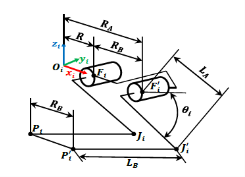
\includegraphics[width=0.5\linewidth]{Main/Chapter4/Images4/Metodo_B_Modelacion_Cinematica_Posicion_5.png}
                  \caption{Puntos y distancias geométricas para la solución de la cinemática de velocidad del método B \cite{Path_Planning_and_Trajectory_Optimization}.}
                  \label{f:Cap4_Metodo_B_Modelacion_Cinematica_Posicion_5}
            \end{figure}  
        
                    \newpage

        
        Definiendo en términos de $\overrightarrow{s_i}$ el vector $\overrightarrow{\xi}_{J_iP_i}$ , la ecuación \eqref{eq:cap4_MB_1111} se puede escribir como:
        \begin{equation} 
            \overrightarrow{s_{i}}^T \cdot \overrightarrow{s_{i}} - L_{B}^{2} = 0
            \label{eq:cap4_MB_11}
        \end{equation} 

    Donde: 
    \begin{align}
        \overrightarrow{s_{i}} & = \overrightarrow{P_{0}}- \left(\overrightarrow{F_{i}}+\overrightarrow{\xi_{F_{i}J_{i}}} \right)\\&= 
            \begin{bmatrix}
                P_{0x} \\
                P_{0y} \\
                P_{0z}
            \end{bmatrix} -  R_{i}^{R}
            \left( 
            \begin{bmatrix}
                R \\
                0\\
                0
            \end{bmatrix} + 
            \begin{bmatrix}
                L_{A} \cos(\theta_i) \\
                0\\
                -L_{A} \sin(\theta_i) 
            \end{bmatrix}
            \right)
        \label{eq:cap4_MB_12}
    \end{align}


    En la ecuación \eqref{eq:cap4_MB_12}, $[P_{0x},P_{0y},P_{0z}]$ es la posición del efector final $\overrightarrow{P_{0}}$ , y el superíndice $R$ es el marco de referencia local $O-xyz$ como se muestra en la figura \eqref{f:Cap4_Metodo_B_Modelacion_Cinematica_Posicion_5}. $R$ es la diferencia entre ${R}_{A}$ y ${R}_{B}$.
    Debido a la simetría en la estructura del robot paralelo delta, cada brazo se puede tratar por separado. Cada brazo está separado por un ángulo de 120° grados y la posición del sistema de referencia correspondiente para cada brazo $O_i - x_i y_i z_i$  es el mismo que el superindice $R$ pero girado en un ángulo para cada brazo $i\in\{1,2 ,3\}$, respectivamente. 
    La matriz de transformación  o  la  matriz de rotación se indica en la ecuacion \eqref{eq:cap4_MB_13}.
    
       \begin{equation}
         R_{i}^{R} =
        \begin{bmatrix}
                \cos(\varphi_i)&-\sin(\varphi_i)&0 \\
                \sin(\varphi_i)&\cos(\varphi_i)&0 \\
                0&0&1
            \end{bmatrix}
        \label{eq:cap4_MB_13}
    \end{equation}  
    
            \begin{figure}[htb]
                 \centering
                 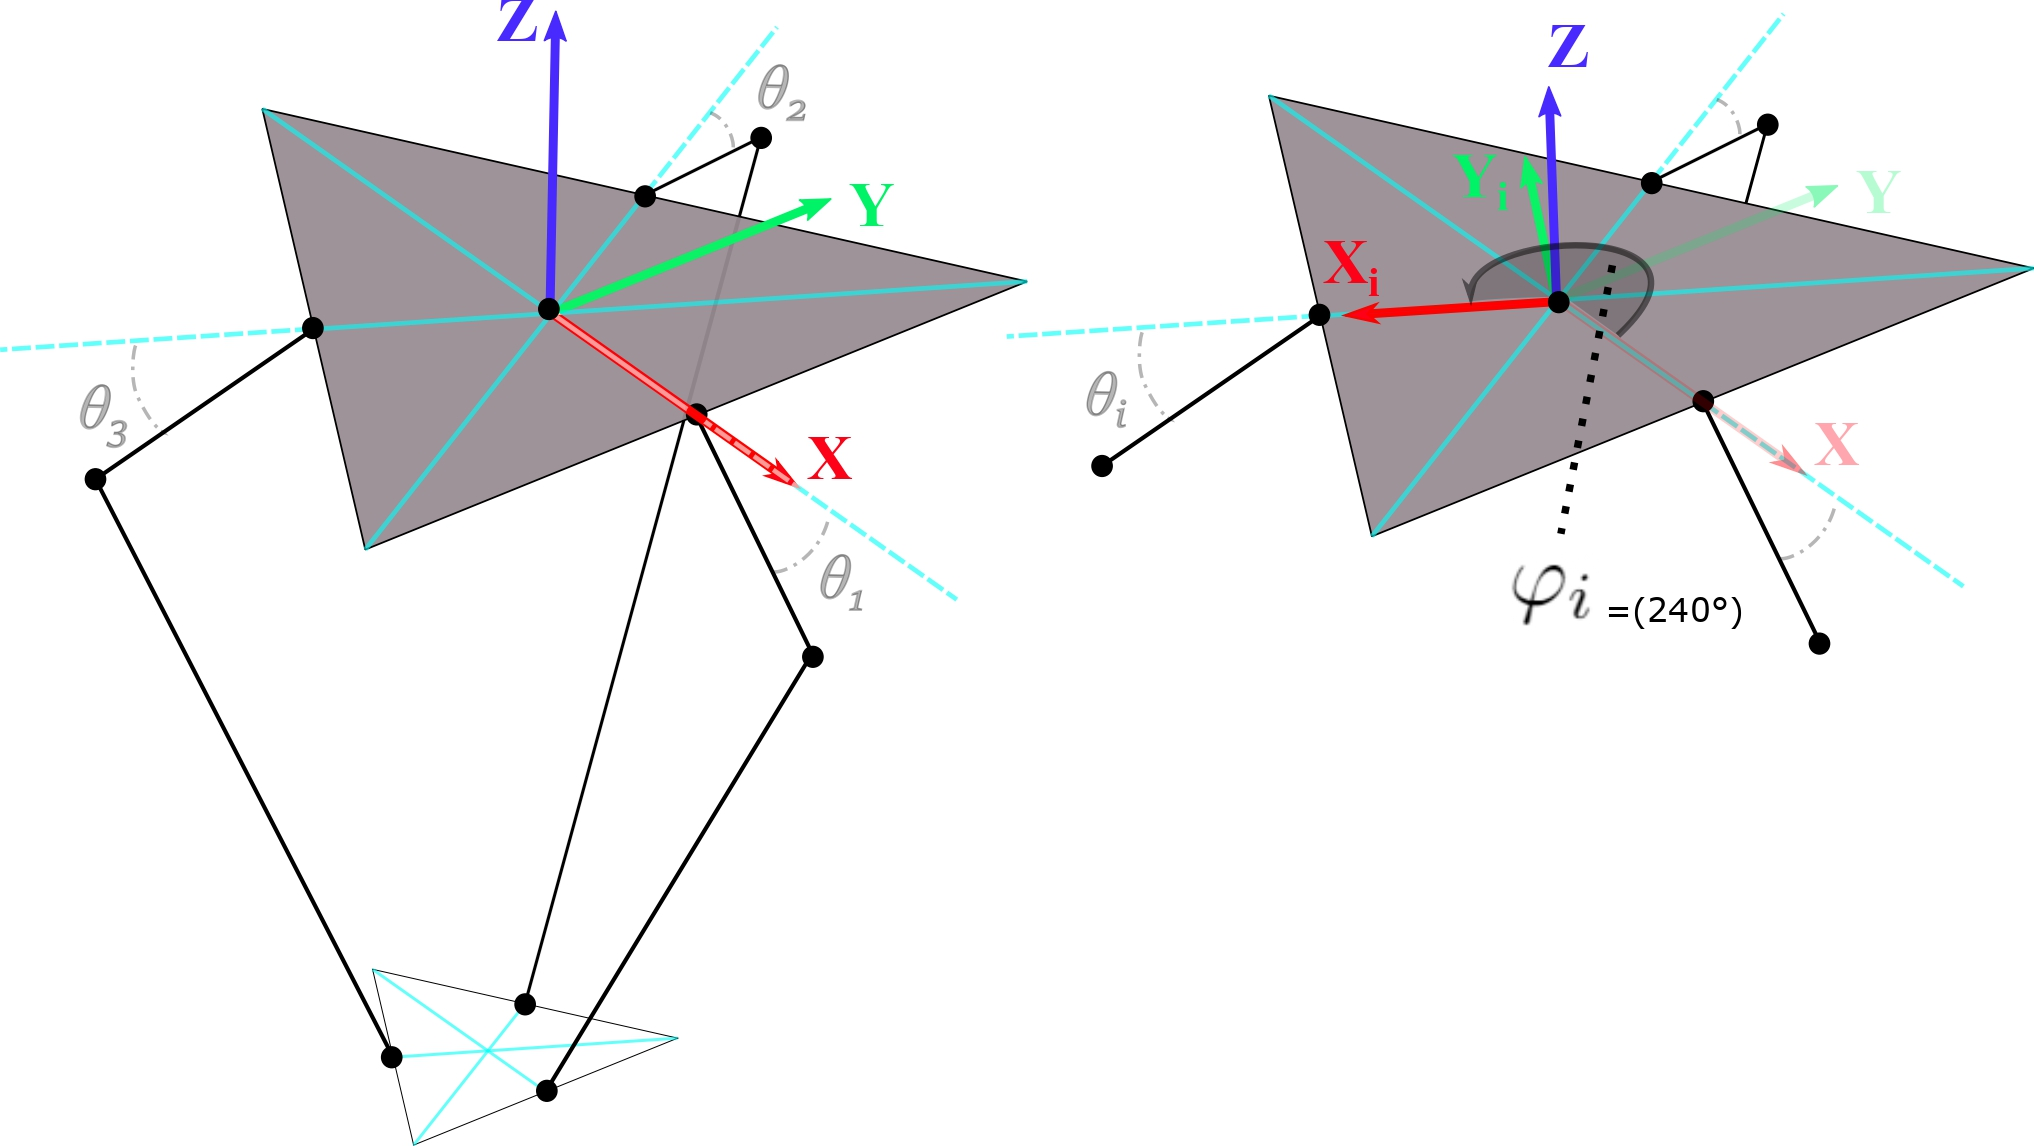
\includegraphics[width=0.9\linewidth]{Main/Chapter4/Images4/DIBUJO33.jpg}
                  \caption{Representación gráfica de la rotación del sistema de coordenadas local $O$-$XYZ$ en los ángulos $\varphi_i \in \{i=1,2,3\}$ }
                  \label{f:Cap4_Metodo_B_Modelacion_Cinematica_Posicion_5asdasdfvtk}
            \end{figure}  
            
            
            
    \newpage

            
    Derivando la ecuación \eqref{eq:cap4_MB_11} para obtener una expresión del jacobiano $J$: 
    
    \begin{equation} 
            \overrightarrow{s_{i}}^T \cdot \overrightarrow{\dot{s}_{i}}= 0
            \label{eq:cap4_MB_1141}
        \end{equation} 
    
    Donde la derivada temporal del término $\overrightarrow{{s}_{i}}$ viene dada por:
    
    \begin{equation}
            \overrightarrow{\dot{s}_{i}}=\begin{bmatrix}
                \dot{P}_{0x} \\
                \dot{P}_{0y} \\
                \dot{P}_{0z}
            \end{bmatrix} +  R_{i}^{R}
            \begin{bmatrix}
                L_{A} \sin(\theta_i) \\
                0\\
                L_{A} \cos(\theta_i) 
            \end{bmatrix} \dot{\theta}_i = \overrightarrow{\dot{P}_0}+\overrightarrow{b_i}\dot{\theta}_i ~~; i \in \{1,2,3\}
        \label{eq:cap4_MB_12112}
    \end{equation}
    
    Remplazando la ecuación \eqref{eq:cap4_MB_12112} en la ecuación  \eqref{eq:cap4_MB_1141}:
    
        \begin{equation}
         \begin{bmatrix}
                \overrightarrow{s_{1}}^T \\
                \overrightarrow{s_{2}}^T \\
                \overrightarrow{s_{3}}^T
            \end{bmatrix}\overrightarrow{\dot{P}_0} +\begin{bmatrix}
                \overrightarrow{s_{1}}^{T} \cdot \overrightarrow{b_{1}} &0&0\\
                0 &\overrightarrow{s_{2}}^{T}\cdot \overrightarrow{b_{2}}&0\\
                0 &0&\overrightarrow{s_{3}}^{T}\cdot \overrightarrow{b_{3}}
            \end{bmatrix}\overrightarrow{\dot{\theta}_i} =         \begin{bmatrix}
                0 \\
                0 \\
                0
            \end{bmatrix}
        \label{eq:cap4_MB_12112234}
    \end{equation}
    
   Reordenando con la finalidad de separar los términos de velocidad lineal del efector con los de velocidad angular de los actuadores y usando la definición de la ecuación \eqref{eq:cap4_MB_10}, el jacobiano $J$ es:
    \begin{equation}
        J = -J_{1}J_{2}=-
        {\begin{bmatrix}
                \overrightarrow{s_{1}}^T \\
                \overrightarrow{s_{2}}^T \\
                \overrightarrow{s_{3}}^T
            \end{bmatrix}}^{-1}
        {\begin{bmatrix}
                \overrightarrow{s_{1}}^{T} \cdot \overrightarrow{b_{1}} &0&0\\
                0 &\overrightarrow{s_{2}}^{T}\cdot \overrightarrow{b_{2}}&0\\
                0 &0&\overrightarrow{s_{3}}^{T}\cdot \overrightarrow{b_{3}}
            \end{bmatrix}}
        \label{eq:cap4_MB_14}
    \end{equation}  
    
    Donde:
    \begin{equation}
        \overrightarrow{b_{i}} = R_{i}^{R}             
        \begin{bmatrix}
                L_{A} \sin(\theta_i) \\
                0\\
                L_{A} \cos(\theta_i) 
            \end{bmatrix}
             ~~; i \in \{1,2,3\}
        \label{eq:cap4_MB_15}
    \end{equation}  
    
    En el caso de los robots en serie, la matriz jacobiana es solo una función de los angulos $\overrightarrow{\theta}$   , pero para los robots paralelos, la matriz jacobiana depende de la información del espacio articular $\overrightarrow{\theta}$   así como de la posición cartesiana del efector final $\overrightarrow{P_0}$   .
        \newpage

    \subsection{Modelación cinemática de aceleración}\label{cap4_mb_subsection_acel}
        
        En esta sección se presentan las ecuaciones para determinar la aceleración angular de los actuadores del robot delta. La aceleración se determina derivando 2 veces matricialmente la ecuación \eqref{eq:cap4_MB_11} de la sección \eqref{mb_cvel} de modelación cinemática de velocidad para el método B.
        
        La aceleración angular de los motores del robot delta se calcula con la siguiente formula:
        
        
        \begin{equation}
                    \overrightarrow{\ddot{ \theta }}=J^{-1} \left[ \overrightarrow{\ddot{P_{0}}}+ \left[ \begin{matrix}
                \overrightarrow{s_{1}}^{T}\\
                \overrightarrow{s_{2}}^{T}\\
                \overrightarrow{s_{3}}^{T}\\
                \end{matrix}
                 \right] ^{-1} \ast \left(  \left[ \begin{matrix}
                \overrightarrow{\dot{s}_{1}}^{T}\\
                \overrightarrow{\dot{s}_{2}}^{T}\\
                \overrightarrow{\dot{s}_{3}}^{T}\\
                \end{matrix}
                 \right]  J+K \right) \ast\overrightarrow{\dot{ \theta }} \right]
            \label{eq:cap4_MB_16}
        \end{equation} 

        Donde: 

        \begin{equation}
                 K= \left[ \begin{matrix}
                \overrightarrow{\dot{s}_{1}}^{T}\overrightarrow{b_{1}}+\overrightarrow{s_{1}}^{T}\overrightarrow{\dot{b}_{1}}  &  0  &  0\\
                0  &  \overrightarrow{\dot{s}_{2}}^{T}\overrightarrow{b_{2}}+\overrightarrow{s_{2}}^{T}\overrightarrow{\dot{b}_{2}}  &  0\\
                0  &  0  &  \overrightarrow{\dot{s}_{3}}^{T}\overrightarrow{b_{3}}+\overrightarrow{s_{3}}^{T}\overrightarrow{\dot{b}_{3}}\\
                \end{matrix}
                 \right]  
            \label{eq:cap4_MB_17}
        \end{equation} 
        
        \begin{equation}
                  \overrightarrow{\dot{b}_{i}}= \left[ \begin{matrix}
                L_{A} \cos⁡ \left(  \theta _{i} \right) \\
                0\\
                - L_{A}\sin ⁡ \left(  \theta _{i} \right) \\
                \end{matrix}
                 \right] \overrightarrow{\dot{ \theta _{i}}}  
            \label{eq:cap4_MB_18}
        \end{equation} 
        
        \begin{equation}
                  \overrightarrow{\dot{s}_{i}}= \left[ \begin{matrix}
                \dot{P}_{0x}\\
                \dot{P}_{0y}\\
                \dot{P}_{0z}\\
                \end{matrix}
                 \right] +R_{i}^{R}\ast \left[ \begin{matrix}
                L_{A}\sin  \left(  \theta _{i} \right) \\
                0\\
                L_{A}\cos  \left(  \theta _{i} \right) \\
                \end{matrix}
                 \right] \dot{ \theta _{i}}=\overrightarrow{\dot{P_{0}}}+\overrightarrow{b_{i}}~\dot{ \theta _{i}} 
            \label{eq:cap4_MB_19}
        \end{equation} 

        


        








    \newpage

    \subsection{Modelación dinámica}\label{cap4_mb_subsection_dina}
    
        En esta sección se presenta un método para resolver la dinámica inversa de un robot delta inspirado en los trabajos de Zeeshan Shareef \cite{Path_Planning_and_Trajectory_Optimization}, Collins F. Adetu, Carl A. Moore, Jr. y Rodney G. Roberts \cite{dynamic_omega3}. La modelacion dinámica utiliza como base el principio de trabajo virtual desarrollado por Codourey \cite{Codourey_decoupling}.

 
        
        \subsubsection{Introducción a modelos dinámicos}
    
        El modelo dinámico de manipuladores robóticos juega un papel importante en la optimización de la trayectoria. La principal dificultad para calcular el modelo dinámico es que debe ser realizable y que se pueda calcular en tiempo real. Una forma sencilla de resolver el modelo dinámico de manipuladores paralelos es la cadena cerrada en uniones pasivas. Esta simplificación proporciona relajación en las condiciones de cierre. El modelo dinámico final será la suma de todos los robots individuales así creados. Kleinfinger \cite{kleinfinger1986modelisation} utiliza esta técnica y aplicó los multiplicadores de Lagrange para calcular el modelo dinámico. 
        
        Otro método muy útil para derivar el modelo dinámico de robótica se basa en el principio de trabajo virtual. Según este principio, la contribución de todas las fuerzas inerciales debe ser igual a la contribución de todas las fuerzas no inerciales. Este método simplifica el problema y es igualmente eficiente tanto para robots en serie como en paralelo \cite{Codourey:31400}, \cite{bodyoriente}, \cite{zhang1993efficient}. 
        
        Otra forma de derivar el modelo dinámico es utilizar el principio de trabajo virtual de Lagrange-d’Alembert. Kokkinis y Stoughton \cite{kokkinis1991dynamics}, Nakamura \cite{NakamuraYoshihiko1991Ar} y Wang y Chen \cite{wang1994dynamic} han obtenido con éxito un modelo dinámico que utiliza el principio de trabajo virtual de Lagrange-d’Alembert.
        
        
        Al incorporar todas las masas, la inercia y no linealidades, el modelo dinámico se vuelve muy complicado y computacionalmente costoso, como consecuencia no puede usarse para aplicaciones en tiempo real. Se puede derivar un modelo dinámico practicable para aplicaciones en tiempo real despreciando las masas y la inercia de los antebrazos, propuesto por Ji \cite{StudyinertiaStewart}.
        
       Esta tesis se deriva el modelo dinámico utilizando el principio de trabajo virtual presentado por Codourey \cite{Codourey_decoupling}.      
        \newpage


        \subsubsection{Principio de trabajo virtual}

        Para obtener el torque de los actuadores se emplea el principio del trabajo virtual. El principio establece que, en el equilibrio, el trabajo virtual $\delta W$, realizado por todas las fuerzas externas $F$ que actúan sobre un cuerpo durante cualquier desplazamiento virtual  $\delta r $, consistente con las restricciones estructurales impuestas al cuerpo, es igual a cero. Este principio se ilustra matemáticamente en la ecuacion \eqref{eq:cap4_MB_20}.
        
        \begin{equation}
            \delta W= \sum _{i=1}^{N}F_{i} \ast \delta r_{i}=0\\
            \label{eq:cap4_MB_20}
        \end{equation}

        
        En la ecuación \eqref{eq:cap4_MB_20} solo se consideran las fuerzas externas, todas las fuerzas internas, es decir, las fuerzas de restricción y reacción se ignoran porque estas fuerzas no realizan ningún trabajo virtual. El principio de trabajo virtual se utiliza tradicionalmente para resolver problemas estáticos. Sin embargo, para un sistema que no está en reposo, la fuerza (fuerza de inercia) como resultado de la masa del cuerpo \(m\), que acelera a una tasa \(a\), se incluye en la ecuación \eqref{eq:cap4_MB_20}. Esta extensión del principio de trabajo virtual para casos dinámicos se conoce como principio de D'Alembert \cite{dynamic_omega3}. La ecuación \eqref{eq:cap4_MB_21} es una extensión de  la ecuación \eqref{eq:cap4_MB_20} con la fuerza de inercia incluida:
        
        \begin{equation}
          \delta W= \sum _{i=1}^{N} \left( F_{i}-m_{i}a_{i} \right) \ast \delta r_{i}=0 \\
         \label{eq:cap4_MB_21}
        \end{equation}

        
        Un cuerpo rígido que es capaz de realizar movimientos tanto de traslación como de rotación, por lo tanto la ecuación \eqref{eq:cap4_MB_21} generalmente se escribe como:
        
        \begin{equation}
          \delta W= \sum _{i=1}^{N} \left[  \left( F_{i}-m_{i}a_{i} \right) \ast \delta r_{i}+ \left(  \tau-I\ddot{ \theta } \right) \ast \delta  \theta  \right] =0 \\
         \label{eq:cap4_MB_22}
        \end{equation}
        
        donde,  $\tau $  es el par externo que actúa sobre el cuerpo,  $ I $  es el momento de inercia,  $\ddot{ \theta }$   la aceleración angular y  $ \delta  \theta  $  es el desplazamiento angular virtual.
        
        \newpage


        \subsubsection{Simplificaciones e hipótesis}
        Antes de proceder a derivar el modelo dinámico, existen unas pocas hipótesis para hacer que el modelo sea factible y computacionalmente eficiente. Las hipótesis simplificadoras son:
        
        \begin{itemize}
            \item Debido a que los antebrazos se construyen con materiales ligeros, es posible simplificar el problema dinámico ignorando la inercia rotacional de las varillas paralelas, es decir, se desprecia la inercia rotacional del antebrazo.
            \item Se ignoran los efectos de fricción entra las piezas y la elasticidad de los materiales.
            \item Para fines analíticos, las masas del antebrazo se dividen equitativamente y se colocan en las extremidades. Por lo tanto, la mitad de la masa de la barra está centrada en la extremidad superior (es decir, la junta que una el brazo con el antebrazo), mientras que la otra mitad está centrada en la extremidad inferior (es decir, la junta que une los antebrazos con el efector final). Esta simplificación se muestra en la figura \eqref{f:Cap4_Metodo_B_Modelacion_Dinamica_1}.
        \end{itemize}
        Debido a estas hipótesis, el robot paralelo delta se reduce a los tres brazos y al efector final.
     
        \begin{figure}[H]
              \centering
	          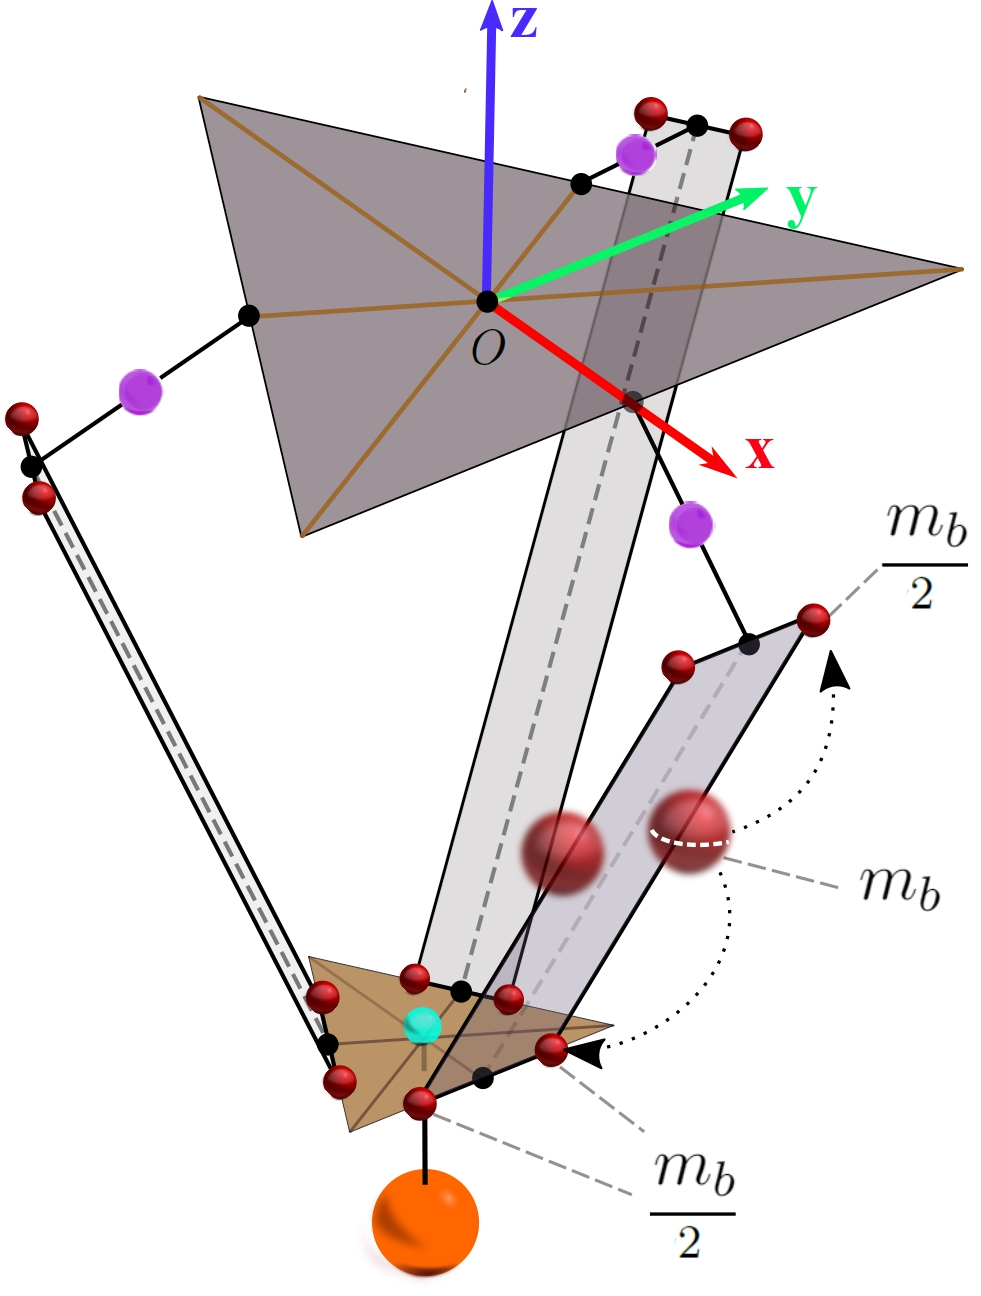
\includegraphics[width=0.5\linewidth]{Main/Chapter4/Images4/DIBUJO39.jpg}
              \caption{Simplificación de masas para la solución de la dinámica inversa del método B.}
              \label{f:Cap4_Metodo_B_Modelacion_Dinamica_1}
        \end{figure}
        
                \newpage


        \subsubsection{Nomenclatura de parámetros geométricos, simplificación de masas y sistema de referencia local }

        En la tabla \eqref{tab:cap4_tabla_13}, la figura \eqref{f:Cap4_Metodo_B_Modelacion_Dinamica_2} y la figura \eqref{f:Cap4_Metodo_B_Modelacion_Dinamica_22} representa la nomenclatura de los parámetros principales para resolver el problema dinámico del robot delta y la simplificación de masas:
        
        \begin{figure}[H]
              \centering
	          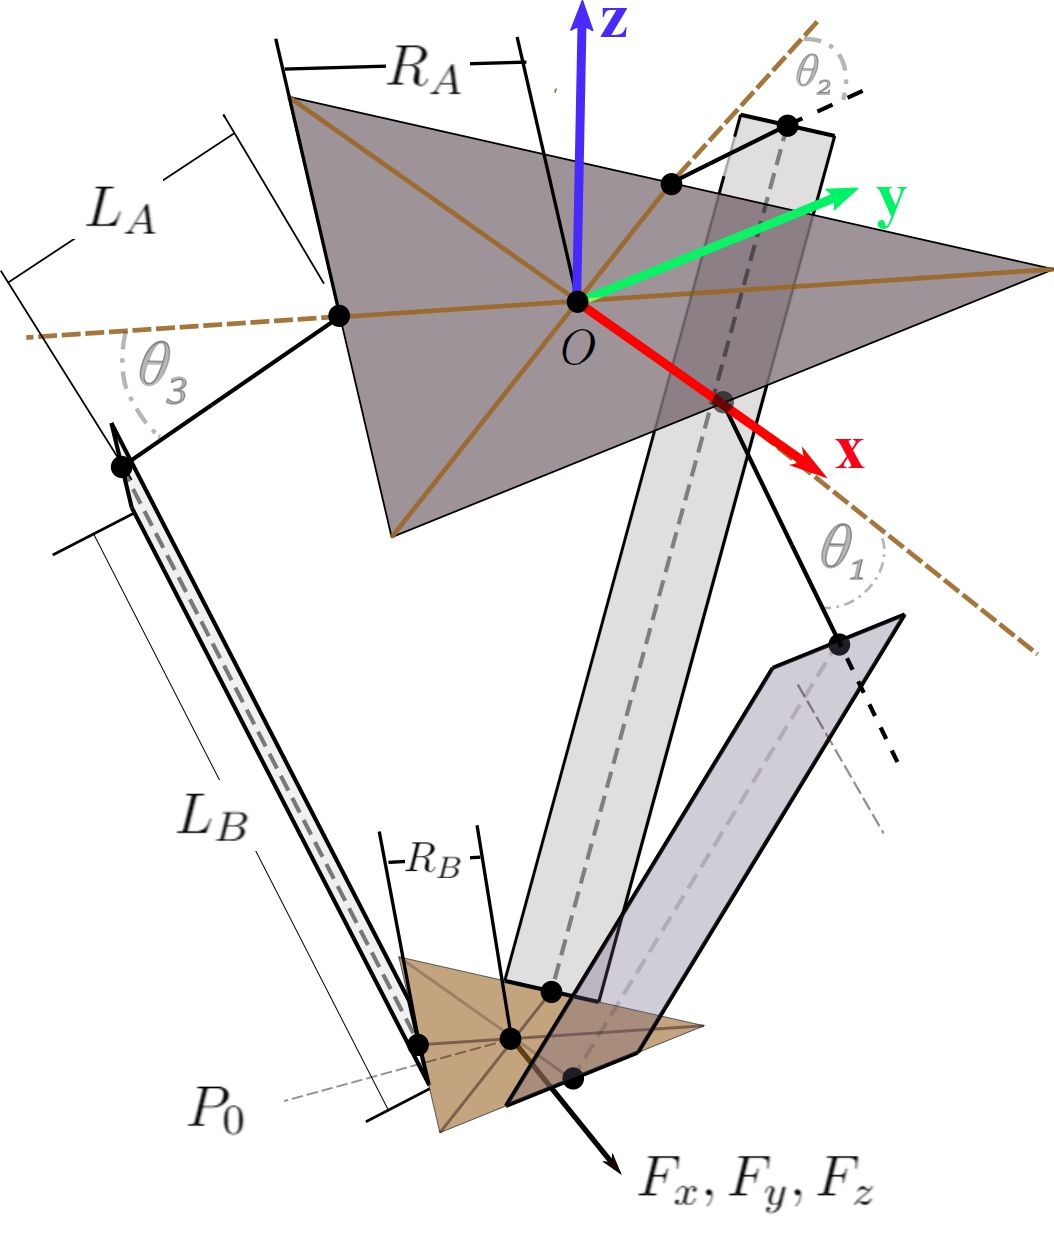
\includegraphics[width=0.55\linewidth]{Main/Chapter4/Images4/DIBUJO36.jpg}
              \caption{Sistema de referencia local y parámetros geométricos para la solución
de la dinámica inversa del método B.}
              \label{f:Cap4_Metodo_B_Modelacion_Dinamica_2}
        \end{figure}

        \begingroup
            \renewcommand{\arraystretch}{1.3}
            \begin{table}[H]
            \centering
            \begin{tabular}{c m{12cm}}
               \hline
               \textbf{Parámetro}  & \multicolumn{1}{c}{\textbf{Descripción}}  \\
               \hline           \hline            
             $L_A$ & Largo del brazo \\
            \hline
             $L_B$ & Largo del antebrazo \\
            \hline
             $R_A$ & Distancia entre el centro de la base fija y la junta revoluta o actuador \\
            \hline
             $R_B$ & Distancia entre el centro del efector a la junta que lo une con el antebrazo\\
            \hline
            ${O} - xyz$ & Sistema de referencia local para resolver el problema dinámico\\
            \hline
             $F_{x},F_{y},F_{z}$ & Fuerzas externas sobre efector final\\
            \hline
            $\theta_i$ & Ángulo del actuador $i \in \{1,2,3\}$\\
            \hline
            $P_0$ & Centroide del efector final\\
            \hline 
            \end{tabular}
            \caption{Parámetros para la solución de la dinámica inversa del método B.}
           \label{tab:cap4_tabla_13}
        \end{table}
        \endgroup     
\newpage

        \begin{figure}[H]
              \centering
	          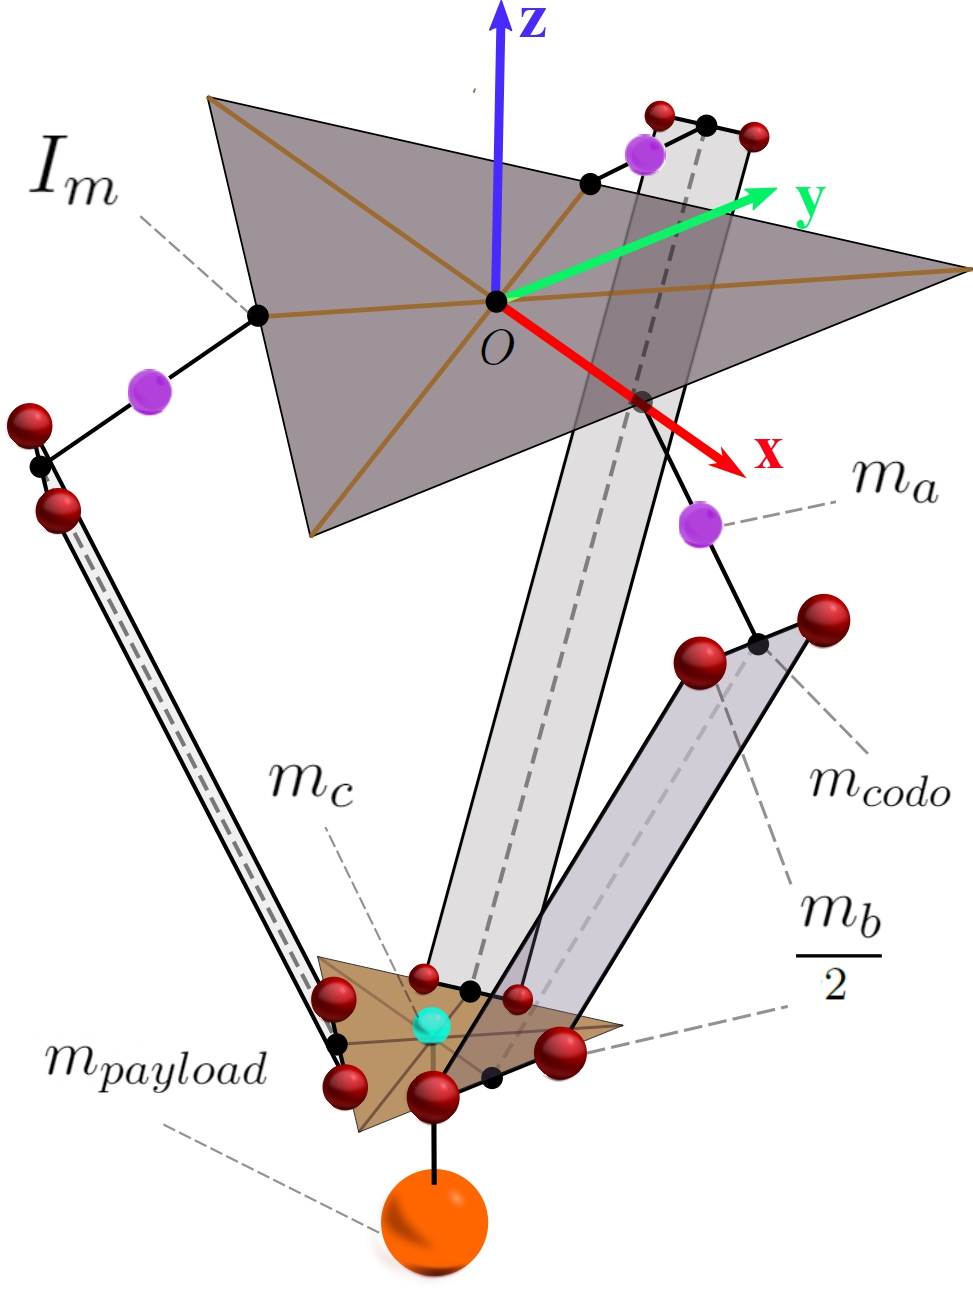
\includegraphics[width=0.63\linewidth]{Main/Chapter4/Images4/DIBUJO37.jpg}
              \caption{Sistema de referencia local y masas para la solución
de la dinámica inversa del método B.}
              \label{f:Cap4_Metodo_B_Modelacion_Dinamica_22}
        \end{figure}

        \begingroup
            \renewcommand{\arraystretch}{1.5}
            \begin{table}[H]
            \centering
            \begin{tabular}{c m{12cm}}
               \hline
               \textbf{Parametro}  & \multicolumn{1}{c}{\textbf{Descripción}}  \\
               \hline           \hline            
            $m_{a}$ & Masa del brazo\\
            \hline
            $m_{b}$ & Masa del antebrazo solo una varilla\\
            \hline
            $m_{c}$ & Masa de la plataforma movil\\
            \hline
            $m_{payload}$ & Masa de objeto adherida a la plataforma móvil que se desea desplazar en una tarea particular\\
            \hline
            $m_{codo}$ & Masa de la junta esférica que unen los brazos con los antebrazos\\
            \hline
            $r$ & Relación de división de masas de los antebrazos para simplificación dinámica\\
            \hline
            $I_{m}$ & Inercia de los motores\\
            \hline
            \end{tabular}
            \caption{Masas, relación de división de masas e inercia de los motores para la solución de la dinámica inversa del método B.}
           \label{tab:cap4_tabla_13333}
        \end{table}
        \endgroup 
\newpage


        \subsubsection{Dinámica inversa}

        Aplicando el principio de trabajo virtual a la simplificación del robot delta, se determinan los torques de los actuadores  $ \overrightarrow{ \tau}= \left[  \tau_{1}, \tau_{2}, \tau_{3} \right] ^{T} $  con la siguiente expresión:
        
        \begin{equation}
             \overrightarrow{ \tau}=I_{b} \overrightarrow{\ddot{ \theta }}+J^{T}m_{nt} \overrightarrow{\ddot{P_{0}}}- J^{T}\overrightarrow{F_{g}}-\overrightarrow{ \tau_{Gb}} 
            \label{eq:cap4_MB_23}
        \end{equation}
        
        Sustituyendo  $ \overrightarrow{\ddot{P_{0}}}=J\overrightarrow{\ddot{ \theta }}+\dot{J} \overrightarrow{\dot{ \theta }} $
        
        \begin{equation}
              \overrightarrow{ \tau}= \left( I_{b}+J^{T} m_{nt} J \right)  \overrightarrow{\ddot{ \theta }}+ \left( J^{T} m_{nt}\dot{J} \right) \overrightarrow{\dot{ \theta }}+ \left( - J^{T}\overrightarrow{F_{g}}-\overrightarrow{ \tau_{Gb}} \right)  
              \label{eq:cap4_MB_24}
        \end{equation}
        
        
        A partir de la ecuación \eqref{eq:cap4_MB_24}, se identificar fácilmente la matriz de masa  $ M \left(  \theta  \right)$, la matriz  $ C \left(  \theta ,\dot{ \theta } \right)  $  de coeficiente de Coriolis y centrífuga, y el vector de términos de gravedad  $ \overrightarrow{G} \left(  \theta  \right)  $  comparándolo con la dinámica estándar:
        
        \begin{equation}
              \overrightarrow{ \tau}=M \left(  \theta  \right) \overrightarrow{\ddot{ \theta }}+C \left(  \theta ,\dot{ \theta } \right) \overrightarrow{\dot{ \theta }}+ \overrightarrow{G} \left(  \theta  \right) 
                \label{eq:cap4_MB_25}
        \end{equation}
        
        
        Dónde:
        \begin{gather}
                 M \left(  \theta  \right) =I_{b}+J^{T} m_{nt} J 
                \label{eq:cap4_MB_26}\\
                 C \left(  \theta ,\dot{ \theta } \right) =J^{T} m_{nt}\dot{J} 
                 \label{eq:cap4_MB_27}\\
                 \overrightarrow{G} \left(  \theta  \right) =- J^{T}\overrightarrow{F_{g}}-\overrightarrow{ \tau_{Gb}}
                 \label{eq:cap4_MB_28}\\
                I_{b}= \left[ \begin{matrix}
                    I_{b1}  &  0  &  0\\
                    0  &  I_{b2}  &  0\\
                    0  &  0  &  I_{b3}\\
                \end{matrix}\right]  
                \label{eq:cap4_MB_29}\\
                I_{bi}=I_{m}+ L_{A}^{2} \left( \frac{m_{a}}{3}+m_{codo}+2\ast r \ast m_{b} \right) \\
                \overrightarrow{\ddot{ \theta }}= \left[ \ddot{ \theta }_{1} \ddot{ \theta }_{2} \ddot{ \theta }_{3}\right] ^{T} 
                \label{eq:cap4_MB_30}\\
                m_{nt}=m_{c}+m_{payload}+3\ast 2 \ast \left( 1-r \right) m_{b} 
                \label{eq:cap4_MB_31}\\
                \overrightarrow{\ddot{P_{0}}}= \left[ \ddot{P}_{0x} \ddot{P}_{0y} \ddot{P}_{0z} \right] ^{T} 
                \label{eq:cap4_MB_32}\\
                \overrightarrow{F_{g}}=m_{nt}  \left[ 0  0  -g \right] ^{T} 
                \label{eq:cap4_MB_33}\\
                \overrightarrow{ \tau_{Gb}}=g \ast CoM\ast \left( m_{a}+m_{codo}+2 \ast r \ast m_{b} \right)  \left[ \cos\left(\theta _{1} \right) \cos  \left(  \theta _{2} \right)  \cos  \left(  \theta _{3} \right)  \right] ^{T} 
                \label{eq:cap4_MB_34}\\
                CoM=L_{A} \frac{\frac{1}{2} m_{a}+m_{codo}+2 \ast r \ast m_{b}}{m_{a}+m_{codo}+2 \ast r \ast m_{b}}
                \label{eq:cap4_MB_35}
        \end{gather}
        
        El detalle de esta sección se encuentra en el anexo \eqref{anexoB}



    \newpage

\section{Espacio de trabajo}

En esta sección se da a conocer la definición de espacio de trabajo por algunos científicos que se han especializado en esta problemática para robots, se presentan de manera general los 2 métodos más utilizados para determinar el espacio y se muestran las restricciones de un robot delta relacionadas con este tema.

    \subsection{Definición}
    En los últimos años, los robots que incluyen una estructura paralela atrajeron la atención de los investigadores del mundo académico. Entre los robots con estructura paralela más famosos se encuentran los provistos de la estructura paralela delta de 3 grados de libertad.  Al comparar los robots que incluyen manipuladores de estructuras en serie con los que incluyen manipuladores de estructuras paralelas, se puede notar que: la estructura paralela tiene una lista de ventajas, como alta rigidez, disponibilidad para transportar objetos más pesados, posicionamiento más preciso, etc. Estas ventajas también vienen dadas por el hecho de que las fuerzas inerciales y de gravedad del objeto manipulado son absorbidas por cada enlace cinemático  \cite{Laribi08}\cite{DASH2005776}. Las desventajas son: espacio de trabajo más estrecho y un control más difícil \cite{DASH2005776}.  
    
    El espacio de trabajo de un robot se define como la región en el espacio cartesiano tridimensional que puede ser alcanzada por un punto de su efector final \cite{LARIBI2007859}, es decir, en el caso de un robot delta, es la región en el espacio tridimensional que puede alcanzar el punto central de su plataforma móvil. 
    
    \begin{figure}[htb]
        \centering
        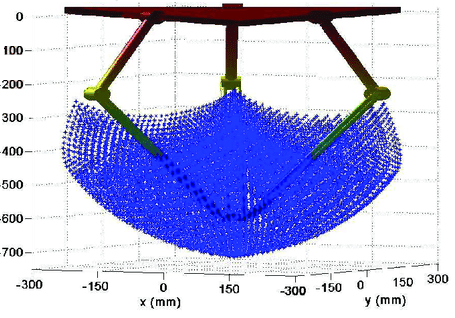
\includegraphics[width=0.7\linewidth]{Main/Chapter4/Images4/wsazul.png}
        \caption{Aproximacion del espacio de trabajo para un robot delta \cite{inproceedingsworkspace1}}
        \label{f:Cap4_ws_1}
    \end{figure}  
    
    \newpage
    
    \subsection{Métodos}
    
    El espacio de trabajo de los robots ha sido estudiado intensamente a lo largo de los años por varios investigadores. Los espacios de trabajo más comunes, según Merlet, son: el espacio de trabajo de traducción, el espacio de trabajo de orientación, el espacio de trabajo accesible, el espacio de trabajo de orientación inclusiva, el espacio de trabajo de orientación total, el espacio de trabajo de destreza, el espacio de trabajo total con orientación reducida \cite{Laribi08} y \cite{AFFI2004311}.
    
    Se han utilizado básicamente las siguientes categorías de métodos para determinar el espacio de trabajo: métodos geométricos y métodos de digitalización, siendo este último el más usado. El método geométrico \cite{delta_Urrea} se basa en obtener un objeto geométrico que describa todas las posibles posiciones del efector final y que satisfagan las restricciones del robot. Se obtiene un objeto geométrico para cada cadena cinemática del robot y el espacio de trabajo es la intersección de los objetos geométricos obtenidos. El método de discretización \cite{delta_Urrea}, que se basa en métodos numéricos, consiste en discretizar el espacio en tres dimensiones, resolviendo la cinemática inversa para cada punto y verificando las restricciones que limitan dicho espacio de trabajo (Ottaviano and Ceccarelli, 2000). La exactitud del volumen de trabajo del robot delta, depende de la probabilidad de que los puntos seleccionados aleatoriamente puedan ser alcanzados por el robot. 
    
    En esta tesis se basa en el método de discretización, sin embargo, será modificado para que el algoritmo calcule la cantidad exacta de los puntos en el espacio que es capaz de alcanzar la plataforma móvil del robot \cite{delta_Urrea}. El algoritmo se basa en la solución de la cinemática directa para todas las posibles combinaciones de los actuadores, obteniendo en cada caso un punto en el espacio cartesiano del centro de la plataforma móvil. El punto pertenece al espacio de trabajo del robot sí y solo sí cumple con todas las restricciones impuestas.
    
        
    \begin{figure}[htb]
        \centering
        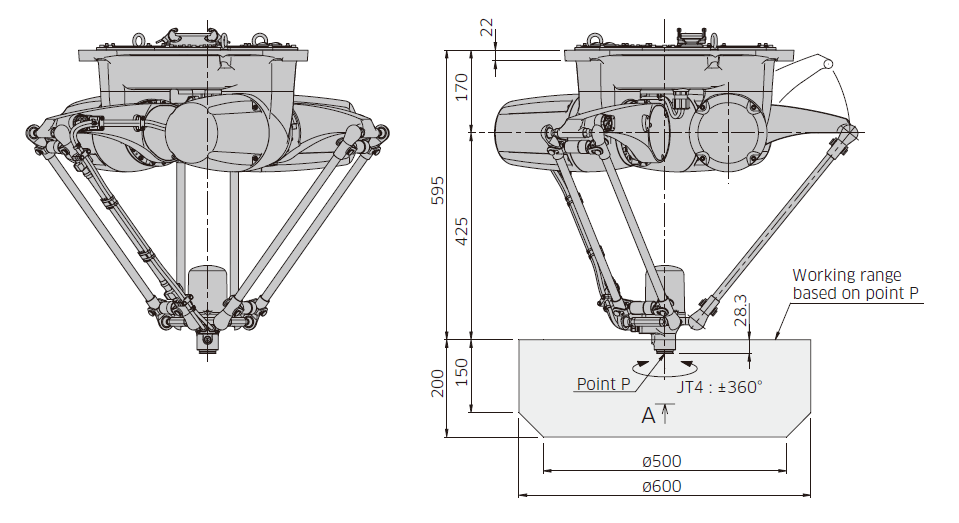
\includegraphics[width=0.8\linewidth]{Main/Chapter4/Images4/abbabb.PNG}
        \caption{Espacio de trabajo YF003N \cite{Kawasakiasd}}
        \label{f:Cap4_ws_2_abb}
    \end{figure} 
    
    
    
    \newpage

    
    \subsection{Tipos de restricciones}\label{restriccionesWS}
    El movimiento de los robots manipuladores dentro del espacio de trabajo puede estar restringido por varios factores, tales como los límites constructivos de los acoplamientos cinemáticos pasivos, los límites dados por los dispositivos de accionamiento de los acoplamientos cinemáticos activos, las cohesiones dadas por los elementos constructivos del robot, así como por puntos o áreas de singularidad que pueden dividir el espacio de trabajo en varios componentes \cite{Laribi08}. 
    
    Las restricciones que se toman en cuenta en este documento para determinar el espacio de trabajo del robot delta son: 
   
    \begin{itemize}
    	\item Limites impuesto en los ángulos de los actuadores [  \(  \theta _{1i,min} \)  -   \(  \theta _{1i,max} \)  ] para cada actuador  \( i \in \{ 1,2,3 \}  \)  .\par
    
    	\item Resolución basada en tamaño del paso de los actuadores, es decir, la discretización del rango impuesto por los límites del punto anterior  \(  \Delta  \theta _{1i} \)  para cada actuador  \( i \in \{ 1,2,3 \}  \) .\par
    
    	\item Restricciones de ángulos internos \(  \theta _{2i} \)  y  \(  \theta _{3i} \) en base a restricción de las juntas o rotulas   .\par
    
    	\item Singularidades que se determinan mediante el determinante del jacobiano  \( J=J_{x}^{-1}J_{ \theta } \)   cuando este es cercano a 0. Estas singularidades son las mismas explicadas en la sección \eqref{CAP4_SINGULARIDAD}.
    	
    	\item Limites comúnmente impuestos por los fabricantes. Generalmente son volúmenes geométricos como cilindros o paralelepípedos.	
    	
    \end{itemize}
    
    
    En la figura \eqref{f:Cap4_ws_2} se visualizan de mejor manera las 5 restricciones impuestas.
    
    
    \begin{figure}[htb]
        \centering
        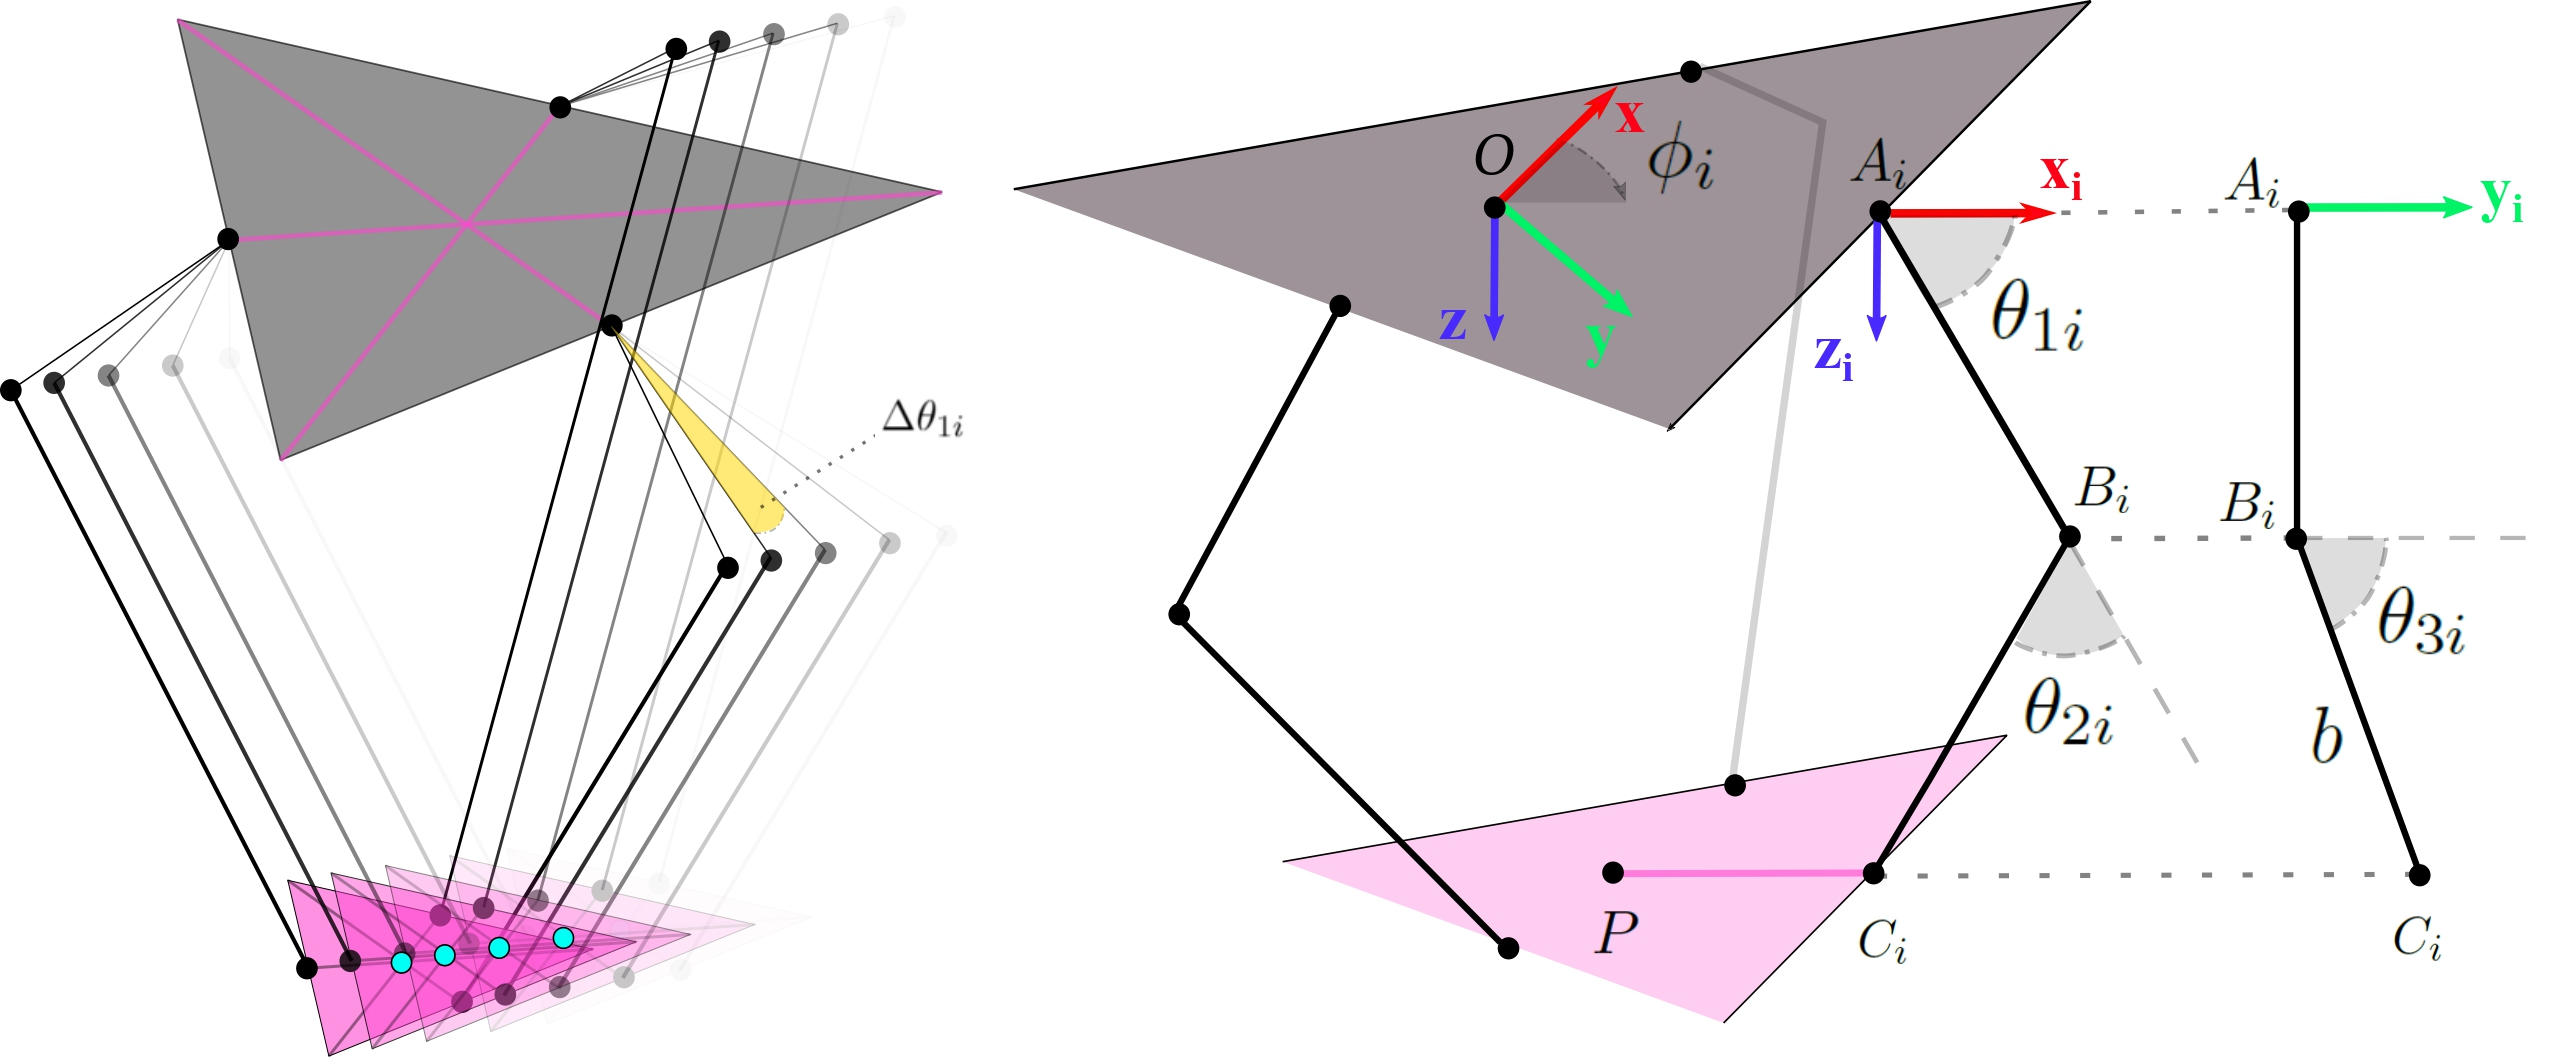
\includegraphics[width=1\linewidth]{Main/Chapter4/Images4/DIBUJO51.jpg}
        \caption{2 tipos de restricciones del espacio de trabajo}
        \label{f:Cap4_ws_2}
    \end{figure}   

    \newpage

\section{Trayectorias}\label{cap4_tray}

    El objetivo principal de esta sección es explicar de manera general la implementación de las trayectorias en robots y dar a conocer detalladamente la trayectoria que se utiliza en este trabajo de grado.
    
    En primer lugar, se define que es una trayectoria, se exponen sus objetivos y se propone un diagrama de flujo con relación a los pasos que se realizan para obtenerlas.
    
    En segundo lugar, se presentan 5 clasificaciones de trayectorias más comunes por los científicos y expertos en robótica para todo tipo de robots.
    
    Finalmente, se describe la trayectoria como la combinación de 2 partes: una descripción puramente geométrica de la secuencia de configuraciones logradas por el robot y una escala de tiempo que especifica los tiempos en que se alcanzan esas configuraciones. A partir del punto de vista anterior, se consideran el caso de las trayectorias punto a punto tanto en el espacio de articulaciones como en el espacio de cartesiano.
    
    \subsection{Definición de trayectorias}
        Un camino geométrico $p$ es un conjunto de puntos en el espacio articular o cartesiano que un manipulador de un robot debe seguir, en otras palabras, es una descripción puramente geométrica. La ecuación \eqref{eq:cap4_tray_1} representa un camino geométrico en el espacio cartesiano: 

        \begin{equation}
            p(s) = [x(s), y(s), z(s)]^T
        \label{eq:cap4_tray_1}
    \end{equation}  
    
    Una trayectoria es un camino geométrico $p(s)$  más consideraciones temporales $s(t)$ . Estas consideraciones temporales pueden estar restringidas por velocidades o aceleraciones impuestas a lo largo del camino. Usualmente se escoge un camino y luego se escoge la ley temporal para la trayectoria.
    
    \begin{equation}
            p(s(t)) = [x(s(t)), y(s(t)), z(s(t))]^T
        \label{eq:cap4_tray_2}
    \end{equation}  
    
    
    \begin{figure}[htb]
        \centering
        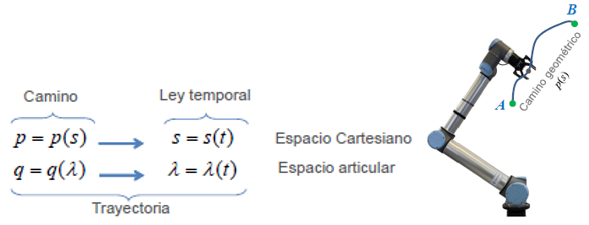
\includegraphics[width=0.7\linewidth]{Main/Chapter4/Images4/cap4_tray_1.png}
        \caption{Descomposición de trayectoria en camino + ley temporal \cite{tray_utec}}
        \label{f:Cap4_tray_1}
    \end{figure}    
    
    \newpage
    
    \subsection{Nomenclatura de trayectorias}
        Un camino geométrico $\theta(s)$ esta en función de un parámetro de camino escalar $s$, que asume que es $0$ al comienzo del camino y $1$ al final, en un punto en el espacio de configuración del robot $\Theta$.
        
    \begin{equation}
        \theta: s \rightarrow   \Theta 
        \label{eq:cap4_tray_3}
    \end{equation}  
    
        \begin{equation}
        \theta: [0;1] \rightarrow   \Theta
        \label{eq:cap4_tray_4}
    \end{equation}
    
    A medida que $s$ aumenta de $0$ a $1$, el robot se mueve a lo largo de la trayectoria. A veces, $s$ se toma como tiempo y se permite que varíe desde el tiempo $s=0$ hasta el tiempo total de movimiento $s=T$, pero a menudo es útil separar el papel del parámetro de trayectoria geométrica $s$  del parámetro de tiempo $t$. Una escala de tiempo $s(t)$ se le asigna un valor $s$ a cada tiempo $t$ $ \in [0; T]$:

    \begin{equation}
        s: t \rightarrow   [0;1] 
        \label{eq:cap4_tray_5}
    \end{equation}  
    
        \begin{equation}
        s: [0; T] \rightarrow   [0;1] 
        \label{eq:cap4_tray_6}
    \end{equation}


    Juntos, un camino geométrico $\theta(s)$ y una escala de tiempo $s(t)$  definen una trayectoria $\theta(s(t))$  o $\theta(t)$   para abreviar. Usando la regla de la cadena, la velocidad y la aceleración a lo largo de la trayectoria se pueden escribir como:


    \begin{equation}
        \dot{\theta} = \frac{d\theta}{ds} \dot{s}
        \label{eq:cap4_tray_7}
    \end{equation}  
    
        \begin{equation}
        \ddot{\theta} = \frac{d\theta}{ds} \ddot{s} + \frac{d^2\theta}{ds^2} \dot{s}^2
        \label{eq:cap4_tray_8}
    \end{equation}


    Para asegurar que la aceleración del robot (y por lo tanto la dinámica) esté bien definida, $\theta(s)$ y $s(t)$ deben ser dos veces diferenciales.

    \newpage
    
    \subsection{Objetivo y procedimiento de generación de trayectorias}
    
    El control cinemático en robótica es una herramienta que permite establecer cuáles son las trayectorias que debe seguir cada articulación del robot a lo largo del tiempo para conseguir los objetivos fijados por el usuario, tales como:
    
    \begin{itemize}
        \item 	Punto de destino
         \item  Tipo de trayectoria del extremo
         \item  Tiempo total invertido

    \end{itemize}
    
    
    Para ello es necesario tomar en cuenta las restricciones físicas de los accionamientos y criterios de calidad tales como sensibilidad, precisión, repetitividad, etc.
    
    Un procedimiento típico para la generación de trayectorias en robots es el que se aprecia en la figura \eqref{f:Cap4_tray_3}:
    
    \begin{figure}[htb]
        \centering
        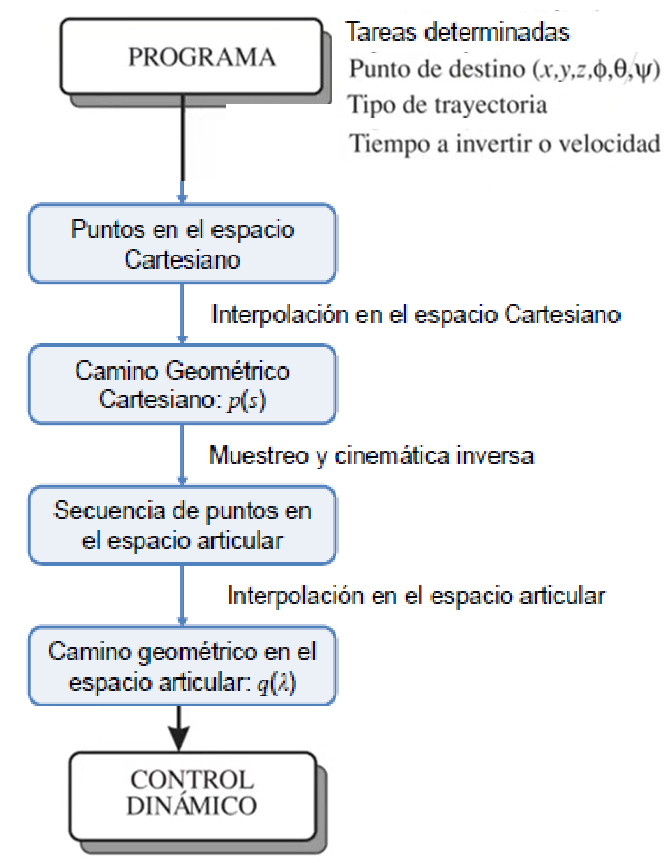
\includegraphics[width=0.65\linewidth]{Main/Chapter4/Images4/cap4_tray_3.png}
        \caption{Procedimiento típico para generar trayectorias \cite{tray_utec}}
        \label{f:Cap4_tray_3}
    \end{figure}  
    
    

        \newpage

    \subsection{Clasificación de trayectorias}
        En esta sección se presentan 5 clasificaciones mas utilizadas para agrupar las trayectorias todo tipo de robots:
        
        \subsubsection{Según el espacio }
            Según la importancia que se le asigna al camino de la trayectoria de un brazo robótico o un efector final de un punto inicial a un punto final en una tarea específica, se pueden dividir en 2 grupos: trayectorias cartesianas y trayectorias articulares. Las trayectorias cartesianas se utilizan cuando es necesario que el robot siga una determinada trayectoria geométrica. Acerca de estas trayectorias, es importante recalcar que sirven para evitar obstáculos, la visualización del camino generado es más fácil y requiere de cinemática inversa. Por el contrario, las trayectorias articulares se ocupan cuando se requiere ir de un punto a otro sin importar la trayectoria. 
            
           \begin{figure}[htb]
             \centering
             \label{f:cap4_tray_4a}
                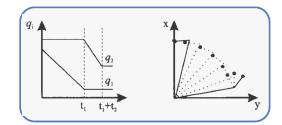
\includegraphics[width=0.8\textwidth]{Main/Chapter4/Images4/cap4_tray_4a.png}
             \caption{Interpolación articular no coordinada \cite{tray_utec}}
        \end{figure}            


           \begin{figure}[htb]
             \centering
             \label{f:cap4_tray_4b}
                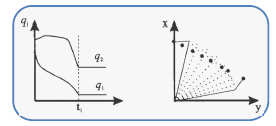
\includegraphics[width=0.8\textwidth]{Main/Chapter4/Images4/cap4_tray_4b.png}
             \caption{Interpolación en el espacio cartesiano \cite{tray_utec}}
        \end{figure}         
            
            
         \newpage   
        
        \subsubsection{Según la geometría del camino }
            El punto de vista principal de esta clasificación es en la forma de la función que representa la trayectoria, ya sea cartesiana o articular. Existen muchos tipos, algunos de estos son:
            \begin{itemize}
                \item         Trayectorias rectilíneas
                \item        Trayectorias polinomiales
                \item        Trayectorias exponenciales
                \item        Trayectorias cicloides
            \end{itemize}
                
        \begin{figure}[htb]
            \centering
            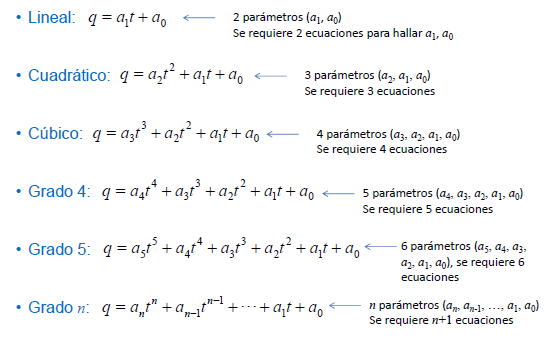
\includegraphics[width=1\linewidth]{Main/Chapter4/Images4/cap4_tray_5.png}
            \caption{Polinomios \cite{tray_utec}}
            \label{f:Cap4_tray_5}
        \end{figure}              
            
        \newpage   

        
        \subsubsection{Según la ley temporal }
            Esta clasificación se basa en las especificaciones de puntos en el camino (velocidades, posición donde detenerse), restricciones impuestas por los actuadores o tareas especificadas (máximo torque, máxima velocidad) o en considerar criterios de optimización (mínimo tiempo, mínima energía o una combinación de ambos).  Ejemplos de aquellas son:
            \begin{itemize}
                \item   Trayectorias tipo bang-bang (on/off) en aceleración
                \item   Trayectorias trapezoidales en velocidad
                \item   Trayectorias polinomiales
            \end{itemize}
            
           \begin{figure}[htb]
             \centering
              \subfloat[Posición]{
             \label{f:cap4_tray_6a}
                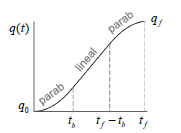
\includegraphics[width=0.5\textwidth]{Main/Chapter4/Images4/cap4_tray_6a.png}}
              \subfloat[Velocidad]{
             \label{f:cap4_tray_6b}
                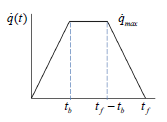
\includegraphics[width=0.5\textwidth]{Main/Chapter4/Images4/cap4_tray_6b.png}}
             \caption{Trayectorias Punto a Punto
: Interpolador de Velocidad Trapezoidal \cite{tray_utec}}
             \label{f:cap4_tray_6}
        \end{figure}            
            
            
            
        
        \subsubsection{Según la coordinación }
            Esta categoría toma toda la atención a la sincronía que tienen las articulaciones en un desplazamiento de un robot de un punto a otro. Se puede dividir en dos grupos: trayectorias coordinadas e independientes. Las trayectorias coordinadas se refieren a que todas las articulaciones inician y terminan el movimiento al mismo tiempo y en simultáneo, mientras que las trayectorias independientes el movimiento de cada articulación es independiente.
        
                 \newpage   

        
        
        \subsubsection{Según el tipo de tarea }
            Dependiendo de la tarea que se quiera realizar, se pueden subdividir en 3 tipos las trayectorias según los puntos por los que debe recorrer el efector final o el ultimo brazo del robot en el espacio cartesiano o articular:

            \begin{itemize}
                \item 	 Trayectorias punto a punto: ir de un punto a otro sin importar la trayectoria 
                \item 	 Trayectorias de puntos vías: ir de un punto a otro, pero pasando por puntos intermedios
                \item 	 Trayectorias continuas (continuidad de velocidad, aceleración): ir de un punto a otro por una trayectoria especifica teóricamente de puntos infinitos
            \end{itemize}
        

    \subsection{Trayectorias punto a punto}
        El tipo de movimiento más simple es desde el reposo en una configuración hasta el reposo en otra. A esto lo llamamos movimiento de punto a punto. El tipo de trayectoria más simple para el movimiento de punto a punto es una línea recta. Las rutas en línea recta y sus escalas de tiempo se analizan a continuación. Las ideas en esta seccion son extraidas del libro creado por los academicos de la Universidad de Northwestern  \cite{moder_robot}.
    
        \subsubsection{Trayectorias en Linea Recta}
            Una línea recta comienza con una configuración inicial $\theta_{inicio}$ hasta una configuración final $\theta_{fin}$ que pueden ser definidas en espacio de articulaciones o en espacio cartesiano. La línea recta se puede escribir: 
        
            \begin{equation}
                \theta(s)= \theta_{inicio} + s(\theta_{fin}-\theta_{inicio}) ; s \in [0,1]
                \label{eq:cap4_tray_9}
             \end{equation}
            
            Sus derivadas son:
            \begin{equation}
                \frac{d\theta}{ds}=\theta_{fin}-\theta_{inicio}
                \label{eq:cap4_tray_10}
             \end{equation}      
            \begin{equation}
                \frac{d^2\theta}{ds^2}=0
                \label{eq:cap4_tray_11}
             \end{equation}  
            
            Las líneas rectas en el espacio articular generalmente no producen un movimiento en línea recta del efector final en el espacio cartesiano. Si se desean movimientos en línea recta en el espacio cartesiano, $X_{inicio}$ y $X_{fin}$ pueden especificar las configuraciones de inicio y finalización. Si $X_{inicio}$ y $X_{fin}$ están representados por un conjunto mínimo de coordenadas, entonces una línea recta se define como:
            
            \begin{equation}
                X(s)= X_{inicio} + s(X_{fin}-X_{inicio}) ; s \in [0,1]
                \label{eq:cap4_tray_12}
             \end{equation}    
                
            \begin{figure}[htb]
                \centering
                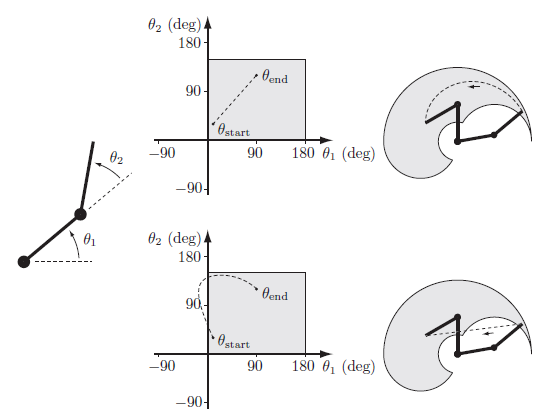
\includegraphics[width=1\linewidth]{Main/Chapter4/Images4/cap4_tray_7.png}
                \caption{(Izquierda) Un robot 2R con límites de articulación $0^{\circ} \leq \theta_1 \leq 180^{\circ}$
, $0^{\circ} \leq \theta_2 \leq 150^{\circ}$. (Centro superior) Una trayectoria en línea recta en el espacio articular y (arriba a la derecha) el movimiento correspondiente del efector final en el espacio de la tarea (línea discontinua). Las configuraciones de punto final alcanzables, sujetas a límites de articulación, se indican en gris. (Centro inferior) Esta línea curva en el espacio de la articulación y (parte inferior derecha) la trayectoria de la línea recta correspondiente en la línea discontinua del espacio de la tarea) violaría los límites de la articulación. \cite{moder_robot}}
                \label{f:Cap4_tray_7}
            \end{figure}  
            
        En comparación con el caso en el que se utilizan coordenadas articuladas, se deben abordar las siguientes cuestiones:
        \begin{itemize}
                \item Si el camino pasa cerca de una singularidad cinemática, las velocidades de las articulaciones pueden volverse excesivamente grandes para la mayoría de las escalas de tiempo del camino.
                \item Dado que el espacio de trabajo en el que se desenvuelve el efector final de un robot puede no ser convexo en coordenadas X, algunos puntos en una línea recta entre dos puntos finales alcanzables pueden no ser accesibles. 
        \end{itemize}

        \newpage

            
            
            
        \subsubsection{Escala temporal de un camino en línea recta}
            Una escala de tiempo $s(t)$ de una trayectoria debe garantizar que el movimiento sea lo suficientemente suave y que se satisfaga cualquier restricción sobre la velocidad y aceleración del robot. Para una trayectoria en línea recta en el espacio articular de la forma de la ecuacion \eqref{eq:cap4_tray_9}, las velocidades y aceleraciones articulares escaladas en el tiempo son respectivamente:
        
        
            \begin{equation}
                \dot{\theta}=\dot{s} (\theta_{fin}-\theta_{inicio})
                \label{eq:cap4_tray_13}
             \end{equation}      
             
            \begin{equation}
                \ddot{\theta}=\ddot{s} (\theta_{fin}-\theta_{inicio})
                \label{eq:cap4_tray_14}
             \end{equation}  
        
    Para un camino en línea recta en el espacio cartesiano parametrizado por un conjunto mínimo de coordenadas $X\in{\Re}^m$, simplemente se reemplaza $\theta$, $\dot{\theta}$,$\ddot{\theta}$ por $X$, $\dot{X}$,$\ddot{X}$ .        
        
        \paragraph{Escala de tiempo polinomial}
        
            Una forma conveniente para la escala de tiempo $s(t)$ es un polinomio cúbico en función del tiempo: 
            
            \begin{equation}
                s(t)= a_{0}+a_{1}t+a_{2}t^{2}+a_{3}t^{3}
                \label{eq:cap4_tray_15}
             \end{equation}     
        
            Un movimiento de punto a punto desde el tiempo $0$ al  $T$ imponer las restricciones iniciales:
        
            \begin{equation}
                s(0)= \dot{s}(0) = 0 
                \label{eq:cap4_tray_16}
             \end{equation} 
             
             y las restricciones terminales:
             
            \begin{equation}
                s(T) = 1 
                \label{eq:cap4_tray_17}
             \end{equation} 
            \begin{equation}
                \dot{s}(T) = 0 
                \label{eq:cap4_tray_18}
             \end{equation}         
             
            Derivando la ecuación \eqref{eq:cap4_tray_15}:
            \begin{equation}
                \dot{s}(t)= a_{1}+2a_{2}t+3a_{3}t^{2}
                \label{eq:cap4_tray_19}
             \end{equation}     
            
        Evaluando la ecuación \eqref{eq:cap4_tray_19} en  $t = 0$ , $t = T$ y resolviendo las cuatro restricciones representadas por las ecuaciones  \eqref{eq:cap4_tray_16},\eqref{eq:cap4_tray_17} y \eqref{eq:cap4_tray_18} :
        
            \begin{equation}
                 a_{0}=0;a_{1}=0;a_{2}=\frac{3}{T^2};a_{3}=-\frac{2}{T^3}
                \label{eq:cap4_tray_20}
             \end{equation}     
        
        Reemplazando los coeficientes $a_i$ en la ecuación \eqref{eq:cap4_tray_15}: 
        
            \begin{equation}
                s(t)=a_{2}t^{2}+a_{3}t^{3} = (\frac{3}{T^2})t^{2}+(-\frac{2}{T^3})t^{3}
                \label{eq:cap4_tray_21}
             \end{equation}  
             

            Sustituyendo la ecuación \eqref{eq:cap4_tray_21} y sus derivadas en las ecuaciones \eqref{eq:cap4_tray_9},\eqref{eq:cap4_tray_13} y  \eqref{eq:cap4_tray_14} :
            
            \begin{equation}
                \theta(t)= \theta_{inicio} + \left(  \frac{3t^{2}}{T^2}-\frac{2t^{3}}{T^3} \right) (\theta_{fin}-\theta_{inicio})            
                \label{eq:cap4_tray_22}
             \end{equation}   
             
            \begin{equation}
                  \dot{\theta}(t)= \left(  \frac{6t}{T^2}-\frac{6t^{2}}{T^3} \right) (\theta_{fin}-\theta_{inicio})
                \label{eq:cap4_tray_23}
             \end{equation} 
             
            \begin{equation}
                \ddot{\theta}(t)= \left(  \frac{6}{T^2}-\frac{12t}{T^3} \right) (\theta_{fin}-\theta_{inicio})
                \label{eq:cap4_tray_24}
             \end{equation} 
             
             \begin{figure}[htb]
                \centering
                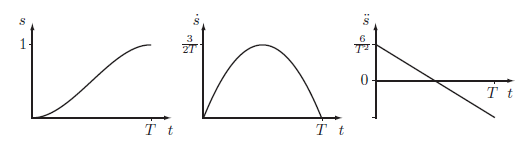
\includegraphics[width=0.8\linewidth]{Main/Chapter4/Images4/cap4_tray_8.png}
                \caption{Gráficas de $s(t)$, $\dot{s}(t)$ y $\ddot{s}(t)$ para una escala de tiempo polinomial de tercer orden \cite{moder_robot} }
                \label{f:Cap4_tray_8}
            \end{figure}  
             
             
        Las velocidades máximas de la articulación se alcanzan en el punto medio del movimiento, $t = T/2$ : 
        
            \begin{equation}
                  {\dot{\theta}}_{max}= \frac{3}{2T} (\theta_{fin}-\theta_{inicio})
                \label{eq:cap4_tray_25}
             \end{equation} 

        Las aceleraciones y desaceleraciones máximas de la articulación se logran en $t = 0$ y $t = T$:
        
            \begin{equation}
                  {\ddot{\theta}}_{max}= \left | { \frac{6}{T^2} (\theta_{fin}-\theta_{inicio})} \right|
                \label{eq:cap4_tray_26}
             \end{equation} 
        
            \begin{equation}
                  {\ddot{\theta}}_{min}= -\left | { \frac{6}{T^2} (\theta_{fin}-\theta_{inicio})} \right|
                \label{eq:cap4_tray_27}
             \end{equation} 
             
        Si existen límites conocidos en las velocidades máximas de la articulación $\left|\dot{\theta} \right|  \leq  {\dot{\theta}}_{limite} $  y las aceleraciones máximas de la articulación  $\left|\ddot{\theta} \right|  \leq  {\ddot{\theta}}_{limite} $ , estos límites se pueden verificar para ver si el tiempo de movimiento solicitado $T$ es factible. Alternativamente, se podría resolver $T$ para encontrar el tiempo de movimiento mínimo posible que satisfaga la restricción de velocidad o aceleración más restrictiva.
        
        \newpage

             
        \paragraph{Perfiles de movimiento trapezoidal}\label{Perfiles_de_movimiento_trapezoidal}
        
        Las escalas de tiempo trapezoidales son bastante comunes en el control motor, particularmente para el movimiento de una sola articulación. El movimiento punto a punto consta de una fase de aceleración constante $\ddot{s}=a$ de tiempo $t_a$, seguida de una fase de velocidad constante $\dot{s}=v$ de tiempo $t = T-2t_a$, seguida de una fase de desaceleración constante $\ddot{s}=-a$ de tiempo $t_a$. El resultado del perfil $\dot{s}$ es un trapezoide y el perfil $s$ es la concatenación de una parábola, un segmento lineal y una parábola en función del tiempo (figura \eqref{f:Cap4_tray_9}).

            \begin{figure}[htb]
                \centering
                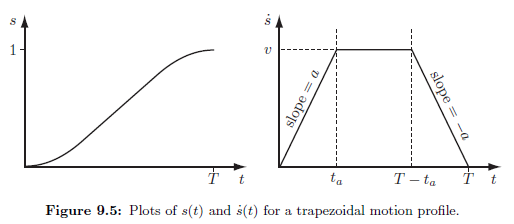
\includegraphics[width=0.7\linewidth]{Main/Chapter4/Images4/cap4_tray_9.png}
                \caption{Gráficas de $s(t)$ y $\dot{s}(t)$ para un perfil de movimiento trapezoidal \cite{moder_robot}}
                \label{f:Cap4_tray_9}
            \end{figure}  
    
        La escala de tiempo trapezoidal no es tan suave como la escala de tiempo cúbico, pero tiene la ventaja, si se saben los límites constantes de las velocidades en las articulaciones  ${\dot{\theta}}_{limite} \in {\mathbb{R}}^n $   y los límites de aceleraciones de las articulaciones ${\ddot{\theta}}_{limite} \in {\mathbb{R}}^n $  , entonces el movimiento trapezoidal usado por la mayor $v$ y $a$  debe satisfacer:
        
        \begin{equation}
             \left| ({\theta}_{final}-{\theta}_{inicio})v \right|   \leq {\dot{\theta}}_{limite}
            \label{eq:cap4_tray_28}
        \end{equation}
        
        \begin{equation}
             \left| ({\theta}_{final}-{\theta}_{inicio})a \right|   \leq {\ddot{\theta}}_{limite}
            \label{eq:cap4_tray_29}
        \end{equation}
        
        Si ${v^2}/a > 1$, el robot nunca alcanza la velocidad $v$  durante el movimiento. El movimiento trifásico de aceleración-velocidad constante-desaceleración se convierte en un movimiento bifásico de aceleración-desaceleración llamado “bang-bang” y el perfil trapezoidal $\dot{s}̇(t)$ de la figura \eqref{f:Cap4_tray_9} se convierte en un triángulo.
        
        \begin{figure}[htb]
                \centering
                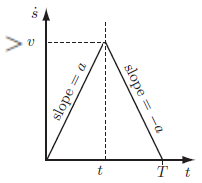
\includegraphics[width=0.3\linewidth]{Main/Chapter4/Images4/cap4_tray_10.png}
                \caption{Bang - bang \cite{moder_robot}}
                \label{f:Cap4_tray_10}
            \end{figure} 
    
    
            \newpage

        Suponiendo que ${v^2}/a \leq 1$ , el movimiento trapezoidal está completamente especificado por $v$,$a$,$t_a$ y  $T$ ,pero solo dos de estos pueden especificarse independientemente ya que deben satisfacer $s(T)=1$  y $v=at_a$ . Es poco probable que se especifique  $t_a$  de forma independiente, por lo que se elimina de las ecuaciones de movimiento mediante la sustitución ${t}_{a}=v/a$ . El perfil de movimiento durante las tres etapas (aceleración, velocidad constante, desaceleración) se puede escribir en términos de $v$,$a$ y $T$ de la siguiente manera:
        
        Para $0 \leq t \leq \frac{v}{a}$ :
        \begin{equation}
            \ddot{s}(t)=a 
            \label{eq:cap4_tray_30}
        \end{equation}
        \begin{equation}
            \dot{s}(t)=at
            \label{eq:cap4_tray_31}
        \end{equation}
        \begin{equation}
             s(t)=\frac{1}{2}at^2
            \label{eq:cap4_tray_32}
        \end{equation}
        
        Para $ \frac{v}{a} \leq t \leq  (T-\frac{v}{a})$ :
        \begin{equation}
            \ddot{s}(t)=0 
            \label{eq:cap4_tray_33}
        \end{equation}
        \begin{equation}
            \dot{s}(t)=v
            \label{eq:cap4_tray_34}
        \end{equation}
        \begin{equation}
             s(t)=vt - \frac{v^2}{2a}
            \label{eq:cap4_tray_35}
        \end{equation}
        
        Para $ (T-\frac{v}{a}) \leq t \leq  T$ :
        \begin{equation}
            \ddot{s}(t)=-a 
            \label{eq:cap4_tray_36}
        \end{equation}
        \begin{equation}
            \dot{s}(t)=a(T-t)
            \label{eq:cap4_tray_37}
        \end{equation}
        \begin{equation}
             s(t)=\frac{2avT-2v^2-a^2(t-T)^2}{2a}
            \label{eq:cap4_tray_38}
        \end{equation}        
        
    Dado que solo dos de $v$, $a$ y $T$ pueden elegirse independientemente, se tiene 3 opciones:
    
    \begin{itemize}
        \item Se elige $v$ y $a$  tal que $v^2/a \leq 1$ , asegurando un perfil trapezoidal de tres etapas y se resuelve $s(T)=1$ para $T$:
        \begin{equation}
            T=\frac{a + v^2}{va}
            \label{eq:cap4_tray_39}
        \end{equation}
        Si $v$ y $a$  corresponden a las mayores velocidades y aceleraciones articulares posibles, este es el tiempo mínimo posible para el movimiento.
        
        \item 	Se elige $v$ y $T$ de modo que $2 \geq vT \geq 1$ , garantizando un perfil trapezoidal de tres etapas y que la velocidad máxima $v$ sea suficiente para alcanzar $s = 1$ en el tiempo $T$. Resolviendo $s(T)=1$   para $a$:
        \begin{equation}
            a=\frac{v^2}{vT-1}
            \label{eq:cap4_tray_40}
        \end{equation}
        
        \item 	Eligiendo $a$ y $T$ tal que $aT^2 \geq 4$ , asegurando que el movimiento sea completo en el tiempo $T$, resolviendo  $s(T)=1$  para $v$ : 
        \begin{equation}
            v=\frac{1}{2}(aT-\sqrt{a}\sqrt{aT^2 - 4})
            \label{eq:cap4_tray_41}
        \end{equation}
    \end{itemize}
        
    Esta misma representación del perfil trapezoidal en esta sección tambien se puede encontrar en el libro \cite{tray_trape}.
    
    }    
        
                \newpage
